%----------------------------------------------------------------------------------------
%	PACKAGES AND OTHER DOCUMENT CONFIGURATIONS
%----------------------------------------------------------------------------------------

\documentclass[11pt]{article} % Default font size is 12pt, it can be changed here
\pagestyle{headings}

\usepackage{geometry} % Required to change the page size to A4
\geometry{a4paper, total={6.4in, 9in}} % Set the page size to be A4 as opposed to the default US Letter
\usepackage{graphicx} % Required for including pictures
\usepackage{subcaption} % to use subfigure
\usepackage{wrapfig} % Allows in-line images such as the example fish picture
\usepackage[natbibapa]{apacite}  % APA Standard citing
\usepackage[ngerman]{babel}
\usepackage[utf8x]{inputenc} % utf8x instead of utf8 becuase "breaks" are not recognized in utf8
\usepackage{parskip} % For auto-paragraphs
\usepackage{color}
\usepackage{amsmath}
\usepackage{lscape} % For landscape content
\usepackage[hyphens]{url} % for linebreaking url's in sources MUSS VOR HYPERREF PACKAGE KOMMEN
\usepackage{hyperref} % For clickable table of contents
\usepackage[bottom]{footmisc} % For footnotes at them bottom
\usepackage{enumitem} % no separation between list items
\usepackage{soulutf8}
\usepackage{lastpage}
\usepackage{fancyhdr}
\usepackage{listings}
\usepackage{multicol}
\usepackage{multirow}
\usepackage{longtable}
\usepackage{tocloft} % allows for sources on figures in the list of figures
\usepackage{pdfpages}
\setlength{\columnsep}{0.6cm}

\pagestyle{fancy}
\renewcommand{\headrulewidth}{0.3pt}
\renewcommand{\footrulewidth}{0.3pt}

\usepackage{titlesec}
\newcommand{\sectionbreak}{\clearpage} % have sections start a new page
\newcommand{\tabitem}{\textbullet~~} % allows for lists inside tabular environment

\hypersetup{
    colorlinks,
    citecolor=black,
    filecolor=black,
    linkcolor=black,
    urlcolor=black
}

\oddsidemargin = 0pt

\makeatletter % Quellen in Abbildungsverzeichnis
\newcommand{\figsourcefont}{\footnotesize Quelle: }
\newcommand{\figsource}[1]{%
  \addtocontents{lof}{%
    {\leftskip\cftfigindent
     \advance\leftskip\cftfignumwidth
     \rightskip\@tocrmarg
     \figsourcefont#1\protect\par}%
  }%
 }
\makeatother

% alle Figures automatisch \centering
\makeatletter
\g@addto@macro\@floatboxreset\centering
\makeatother

% alle Figures und Tabellen automatisch an Position [htb]
\makeatletter
\renewcommand*{\fps@figure}{htb}
\renewcommand*{\fps@table}{htb}
\makeatother

% command für einfacheres Einfügen von einzelnen Bildern
\newcommand{\bild}[4][]{%
  \begin{figure}
    \centering
    \includegraphics[width=#2\textwidth]{#3}%
    \caption{#4}%
    \ifthenelse{\equal{#1}{}}{}{\figsource{\url{#1}}}%
    \label{fig:#3}%
  \end{figure}
}%

\addto{\captionsngerman}{	% Renew some Captions
% \renewcommand*{\contentsname}{Inhalt}
  \renewcommand*{\listfigurename}{Abbildungen}
  \renewcommand*{\listtablename}{Tabellen}
  \renewcommand*{\listoflistingscaption}{Codeblöcke}
  \renewcommand*{\figurename}{Abb.}
  \renewcommand*{\tablename}{Tab.}
  \renewcommand*{\listingscaption}{Code}
}

\usepackage[export]{adjustbox}
\usepackage{caption}
%\usepackage{fixltx2e} % for upper / subscript

\usepackage[scaled]{beramono}
\usepackage[T1]{fontenc}

\usepackage[breakwords]{truncate}


% Swift syntax highlighting code snippets
\usepackage{minted}
\newminted{swift}{ % define a custom minted environment, called with "swiftcode"
  autogobble,     % automatically removes unnecessary indentation
  breaklines,     % automatically breaks long lines on whitespace
  fontsize=\footnotesize, % self explanatory, it's the code's font size
  frame=single,   % add a single line for a frame around the code
  % gobble=2,       % remove first level of indentation (activate in case autogobble fails)
  linenos,        % show line numbers
  numbersep=6pt,  % smaller distance between linenumbers and frame
  style=xcode,    % use Xcode colorscheme
  tabsize=4,      % custom (narrower) indentation
  xleftmargin=15pt, % set left margin, so that the numbers don't hang outside
}
% styling of line number (gray, small, ttfamily)
\renewcommand{\theFancyVerbLine}{\textcolor[rgb]{0.6,0.6,0.6}{\scriptsize \ttfamily{\arabic{FancyVerbLine}}}}
% make inserting code even easier and enable label and caption
\newenvironment{code}[2]
{\VerbatimEnvironment
  \begin{listing}
    \caption{#2}\label{code:#1}
    \begin{swiftcode}%
}{
    \end{swiftcode}
  \end{listing}
}


\newenvironment{italicquotes} % Long quotes italic
{\begin{quote}\itshape}
{\end{quote}}

\linespread{1.2} % Line spacing
\setlength\parindent{0pt} % Uncomment to remove all indentation from paragraphs "Umfang ca..."
% \setcounter{tocdepth}{2} % only show 2 levels of section hierarchy in table of contents

\graphicspath{{images/}} % Specifies the directory where pictures are stored

\begin{document}

%----------------------------------------------------------------------------------------
%	TITLE PAGE
%----------------------------------------------------------------------------------------
\begin{titlepage}

\newcommand{\HRule}{\rule{\linewidth}{0.5mm}} % Defines a new command for the horizontal lines, change thickness here

\center

\textsc{\LARGE Hochschule Luzern\\Informatik}\\[1.5cm] % Name of your university/college
\textsc{\Large Informatikprojekt PAWI, FS 2018}\\[1.5cm] % Major heading such as course name

\HRule \\[1cm]
{\huge \bfseries iOS App mit Augmented Reality}\\[0.6cm] % Title of your document
\HRule \\[1cm]

\vspace{30pt}

\begin{minipage}{0.4\textwidth}
  \begin{flushleft} \large
    \emph{Autoren:}\\
    Dorus \textsc{Janssens}\\
    Lucas \textsc{Schnüriger}\\
    ~\\~ % for vertical alignment
  \end{flushleft}
\end{minipage}
\begin{minipage}{0.4\textwidth}
  \begin{flushleft} \large
    \emph{Dozent:}\\
    Prof. Dr. Ruedi \textsc{Arnold}\\~\\
    \emph{Projektpartner:}\\
    Prof. Dr. Thomas \textsc{Koller}
  \end{flushleft}
\end{minipage}\\[1cm]


\vspace{30pt}

{\large \today }\\[1cm] % Date, change the \today to a set date if you want to be precise

\end{titlepage}


%----------------------------------------------------------------------------------------
%	Vor-Zeugs
%----------------------------------------------------------------------------------------
\pagenumbering{Roman}
\pagestyle{plain}

\IfFileExists{01-Selbststaendigkeitserklaerung}{
  \section*{Selbstständigkeitserklärung}
Hiermit erkläre ich, dass ich die vorliegende Arbeit selbstständig angefertigt und keine anderen als die angegebenen Hilfsmittel verwendet habe. Sämtliche verwendeten Textausschnitte, Zitate oder Inhalte anderer Verfasser wurden ausdrücklich als solche gekennzeichnet.

\vspace{1cm}

Rotkreuz, 8. Juni 2018 

\vspace{2cm}

\parbox{\textwidth}{
  \parbox{7cm}{
    \rule{6cm}{.5pt}\\
    Dorus Janssens
  }
  \hfill
  \parbox{7cm}{
    \rule{6cm}{.5pt}\\
    Lucas Schnüriger
  }
}

}

\newpage
\IfFileExists{02-Abstract}{
  \section*{Abstract}


}

\newpage
\IfFileExists{03-Begriffe}{
  \section*{Begriffe \& Abkürzungen}
\begin{table}
	\begin{tabular}{@{} p{.12\textwidth} p{.85\textwidth} @{}}
		\hline
		\textbf{Begriff} & \textbf{Erklärung} \\
		\hline
		ABIZ	& Forschungsgruppe Algorithmic Business der Hochschule Luzern - Informatik \\
		AR 		& Augmented Reality, computergestützte – primär visuelle – Erweiterung der Realität \\
		cuboro	& Schweizer Unternehmen, das Kugelbahnen aus Holz herstellt \\
		iOS		& Apples mobiles Betriebssystem für iPhones und iPads \\
		ML		& Machine Learning, maschinelles Lernen und Gewinnung von Wissen aus Erfahrungen und Lerndaten durch den Computer \\
		HSLU	& Hochschule Luzern \\
		VR		& Virtual Reality, eine interaktive virtuelle Umgebung, die in Echtzeit generiert wird \\
		WWDC	& Worldwide Developers Conference, jährliche Konferenz von Apple für Software-Entwickler, bei der der Konzern oft neue Produkte vorstellt \\
		Xcode	& Entwicklungsumgebung von Apple zur Entwicklung von Programmen für Apples Betriebssysteme (macOS, iOS, tvOS und watchOS) \\
		\hline
	\end{tabular}
\end{table}

}

%----------------------------------------------------------------------------------------
%	TOC
%----------------------------------------------------------------------------------------
\newpage
\tableofcontents % Include a table of contents

%----------------------------------------------------------------------------------------
%	Content
%----------------------------------------------------------------------------------------
\newpage % Begins the essay on a new page instead of on the same page as the table of contents
\pagenumbering{arabic}

\pagestyle{fancy}
\lhead{I.BA\_PAWI.F18}
\chead{Hochschule Luzern – Informatik}
\rhead{\nouppercase{\leftmark}}
\lfoot{\today}
\cfoot{}
\rfoot{\thepage\ von \pageref{LastPage}}

\newpage
\IfFileExists{04-Einleitung}{
  \section{Einleitung}

In dieser Arbeit sollen die technischen Grenzen von Augmented Reality mit iOS Frameworks aufgezeigt werden. Die Projektmethodik findet im explorativem Verfahren stattfinden. 
Die Arbeit setzt sich zuerst mit der Problemstellung, Ziele und Abgrenzung auseinander. Anschliessend werden die für diese Arbeit relevanten Themen beschrieben und den Stand der Technik in deren Rubrik aufgeführt. Im nächsten Kapitel werden die iOS Frameworks CoreML, Vision, ARKit etc. veranschaulicht. Nach der theoretischen Einleitung werden im Kapitel Lösungsentwicklung die Prototypen vorgestellt, die in der explorativen Phase erstellt wurden. Nach einer Lösungswahl wird im Kapitel Umsetzung ist die erarbeitete Demo-App detailliert dokumentiert. Im anschliessenden Kapitel Validierung wird die erarbeitete Lösung mit dem Anforderungskatalog verglichen und ein technisches Fazit gezogen. Im letzten Kapitel Schlussfolgerung werden die Lessons Learned, persönliche Fazit und ein Ausblick auf weitere Arbeiten gegeben.
% Forschungskonzept, Fragestellung, Method, Aufbau der Arbeit

}

\IfFileExists{05-Problemstellung}{
  \section{Problemstellung}

\subsection{Ausgangslage}
% Welche Problematik führt zu diesem Projekt? Was ist am derzeitigen Zustand unbefriedigend?
Für die PAWI Arbeit im Frühlingssemester 2018 soll eine iOS-App erstellt werden, welche es erlaubt mit einer physischen cuboro Kugelbahn zu interagieren. Einerseits soll es die zu erstellende App erlauben, physische Kugelbahnen digital zu erfassen. Diese Erfassung kann beispielsweise parallel zum Aufbau einer Kugelbahn geschehen, indem die App Bauteil um Bauteil diese zuerst erkennt (mit passenden Methoden aus dem Bereich Bilderkennung/Computer Vision bzw. dem maschinellen Lernen) und dann dessen relative Position innerhalb von der Kugelbahn aufzeichnet. Es sollen zwingend mehrere unterschiedliche Kugelbahnen in der App erfasst sein, ggf. werden diese in der Software fix hinterlegt bzw. können auf einem anderen Weg als mithilfe der App erfasst werden, z.B. durch einen Import aus dem Cuboro-Webkit.

Erfasste Kugelbahnen sollen nach Möglichkeit in AR-Manier als Echtzeit-Überblendung auf Kamerabildern der physischen Kugelbahn projiziert werden können, z.B. indem Bauteile eingefärbt werden, in Form von angezeigten "`Bounding-Boxes"' oder indem virtuelle Kugeln auf der physischen Kugelbahn simuliert werden können. Oder weiter könnten erfasste Kugelbahnen mittels AR beispielsweise auf einen physischen Tisch "`gestellt"' werden und darauf könnte das Rollen von virtuellen Kugeln simuliert werden. 

In dieser Arbeit gibt es einige Freiheitsgrade, sprich viele funktionale und technische Aspekte gilt es zu erarbeiten, evaluieren und fest zu legen. Damit das Endresultat den Erwartungen von Auftraggeber und Betreuer entspricht, sollen Evaluationen und Entscheidungsfindungen in enger Rücksprache mit dem Auftraggeber und dem Betreuer stattfinden. Wichtige Entscheide (wie z.B. Fixierung von funktionalen Anforderungen, Wahl von Frameworks, usw.) müssen vom Auftraggeber bzw. dem Betreuer genehmigt werden, entsprechend sollen diese möglichst proaktiv in Evaluationen, Bau von Prototypen usw. miteinbezogen, sowie über Vor- und Nachteile, Alternativen usw. informiert werden.

\subsection{Ziele}
% Was soll mit dem Projekt erreicht werden? Was soll nach dem Projekt „besser“ sein als vorher?
Das Hauptziel ist es, dass am Schluss eine attraktive und lauffähige Demo-App zur Verfügung steht. Die App soll möglichst intuitiv angewendet werden können und die Möglichkeiten und Grenzen dieser neuen Technologien illustrieren. Weitere Ziele sind das erfolgreiche Einarbeiten in die neue Programmiersprache Swift und den iOS Frameworks Core ML, Vision und ARKit. Die Frameworks sollen anhand von Problemlösungszyklen genauer auf einzelne Aspekte geprüft werden.

\subsection{Abgrenzung (Scope)}
% Welche Sachverhalte sind nicht Bestandteil des Projektes. Welche Restriktionen gibt es im Projekt?
Nichtbestandteil des Projektes sind Betriebssysteme / Frameworks ausserhalb von iOS. Die iOS-App wird ausschliesslich mit Swift entwickelt. Es werden ausschliesslich native iOS UI Komponente für die Applikation verwendet.

\subsection{Fragestellungen}
\begin{itemize}
	\item Das SceneKit eignet sich für 3D Objekte und das SpriteKit für 2D Flächen. Welche der beiden Frameworks kann ein virtuelles Overlay auf einem physischen Würfel erzeugen?
	\item Wie können physische Körper als virtuelle Objekte modelliert werden?
	\item Welche Möglichkeiten bestehen mit augmentierten Objekten zu interagieren und diese zu mutieren?
	\item Wie können virtuelle Objekte ausgerichtet werden?
	\item Wie werden virtuelle Körper definiert, beschrieben, persistiert?
	\item Wie stabil verhält sich der AR Referenzpunkt?
	\item Unter welchen Voraussetzungen kann der Referenzpunkt zuverlässig aufgebaut werden?
\end{itemize}

\subsection{Anforderungen}
Im diesem Kapitel sind alle funktionalen und nichtfunktionalen Anforderungen des Projekts festgehalten. Jede Anforderung ist in eine der folgenden drei Kategorien priorisiert:
\begin{itemize}
	\item Muss (M): Dies sind Festanforderungen, die zwingend vom Projekt erfüllt werden müssen.
	\item Soll (S): Dies sind Wunschanforderungen, die umgesetzt werden sollen, sobald die Muss-Anforderungen erfüllt sind oder erfüllt werden können.
	\item Kann (K): Diese Zusatzanforderungen haben die niedrigste Priorität und können umgesetzt werden, sofern keine anderen (wichtigeren) Anforderungen beeinträchtigt werden und der erfolgreiche Projektablauf nicht gefährdet wird.
\end{itemize}

Die App soll folgende \textbf{Epics} erfüllen:
\begin{enumerate}
	\item \textbf{Bauanleitung:} Der Benutzer kann von einer gewählten Kugelbahn eine Augmented Reality Bauanleitung erhalten, um die Bahn physisch aufbauen zu können.
	\item \textbf{Editor:} Der Benutzer kann in Augmented Reality eine virtuelle Kugelbahn neu erstellen oder eine bestehende verändern, damit diese als Bauanleitung zur Verfügung stehen.
\end{enumerate}

\subsubsection{Funktionale Anforderungen}
In Tabelle \ref{tab:funktionale-anforderungen} sind die funktionalen Anforderungen an die zu entwickelnde App aufgelistet. Diese Anforderungen beschreiben die gewünschten Funktionen und Leistungen der fertigen Anwendung.

\begin{longtable}{l l p{4.7cm} p{8cm}}
	\hline
	\textbf{Nr.} & \textbf{Prio.} & \textbf{Bezeichnung} & \textbf{Erläuterungen} \\
	\hline
	01 & M & Virtuelle Darstellung einer Kugelbahn & Die App kann eine Kugelbahn virtuell darstellen (VR). \\
	02 & M & AR Bahn erstellen & Der Benutzer kann eine virtuelle Kugelbahn in AR erstellen. \\
	03 & M & AR Bahn verändern & Der Benutzer kann eine virtuelle Kugelbahn in AR verändern. \\
	04 & M & AR Bauanleitung & Der Benutzer kann eine physische Kugelbahn mit Hilfe einer AR Bauanleitung Element für Element aufbauen. \\
	05 & M & Mehrere Kugelbahnen erfassen & Die App kann mehrere unterschiedliche Kugelbahnen erfasst, bzw. hinterlegt, haben. \\
	06 & M & Kugelbahn virtuell platzieren & Erfasste virtuelle Kugelbahnen können mittels AR auf eine physische Fläche platziert und betrachtet werden. \\
	07 & S & Virtuelle Überlagerungen einer Kugelbahn & Ein physisches Modell einer Kugelbahn kann in Echtzeit mit virtuellen Überlagerungen auf der App angereichert werden (AR). \\
	08 & K & Virtuelle Kugeln simulieren & Es können virtuelle Kugeln auf einer physischen Kugelbahn simuliert werden. \\
	\hline
	\caption{Funktionale Anforderungen}
	\label{tab:funktionale-anforderungen}
\end{longtable}

\subsubsection{Nichtfunktionale Anforderungen}
In Tabelle \ref{tab:nichtfunktionale-anforderungen} sind die nichtfunktionalen Anforderungen an das Projekt aufgelistet. Nichtfunktionale Anforderungen betreffen einerseits die Qualität (während und ausserhalb der Laufzeit) sowie die Einschränkungen (aus der Technologie und aus Randbedingungen des Moduls PAWI) des Projekts. Dies betrifft sowohl die Applikation als solches, als auch die Dokumentation.

\begin{longtable}{l l p{4.7cm} p{8cm}}
	\hline
	\textbf{Nr.} & \textbf{Prio.} & \textbf{Bezeichnung} & \textbf{Erläuterungen} \\
	\hline
	01 & M & iOS und Swift & Die App ist in Swift für iOS programmiert. \\
	02 & M & Lauffähige App & Die App läuft auf einem iOS Gerät. \\
	03 & M & Recherche von iOS Frameworks & Die Dokumentation enthält Informationen zu den iOS Frameworks ARKit, Core ML und Vision. \\
	04 & M & Technologie aufzeigen & Die App zeigt die Möglichkeiten von AR mittels ARKit auf. \\
	05 & M & Nützlicher Code & Der Sourcecode soll für an der verwendeten Technik interessiert aufschlussreich und hilfreich sein. \\
	\hline
	\caption{Nichtfunktionale Anforderungen}
	\label{tab:nichtfunktionale-anforderungen}
\end{longtable}

\subsection{Lösungsskizze}

}

\IfFileExists{06-Stand-der-Technik}{
  \section{Stand der Technik}

\subsection{Augmented Reality} \label{sub:augmented-reality}
Um zu Verstehen wobei es sich bei Augemented Reality handelt müssen wir den Ursprung des Wortes analysieren. Da augmented soviel wie hinzufügen oder erweitern bedeutet und reality die physische Wahrnehmung der Umgebung wiedergibt kann das Word auf deutsch als erweiterte Realität bezeichnet werden.

Augmented Reality kann wie folgt beschrieben werden: Eine erweiterte Version der Realität, in der direkte oder indirekte die Ansichten physischer Realitätsumgebungen oder Objekte mit überlagerten computergenerierten Bildern über die Sicht eines Benutzers auf die reale Welt projeziert werden, wodurch die aktuelle Wahrnehmung der Realität erweitert wird. (\cite{reality-technologies})

Die AR Technologie hat viele Anwendungszwecke und es wird in der Zukunft eine grosse Rolle spielen. Anbei einige Beispiele damit der Verwendungszweck der Technologie ein klares Bild erhält:
\begin{itemize}
    \item Unterhaltung: Spiele wie Tetris können auf jeder beliebigen Unterlage gespielt werden und von diversen Blichwinkel erlebt werden.
    \item Gesundheitswesen: Dem Arzt werden vitalwerte des Patienten eingeblendet und informationen zur aktuellen operation sowie mögliche Schnittmuster etc. angezeigt.
    \item Wartung: Bei der Wartung von speziellen Turbinensystemen wird der Wartungsarbeiter auf die Herangehensweise aufmerksamgemacht und welche Teile in welcher Reinenfolge abmontiert, gewartet und wiedermontiert werden müssen.
    \item Navigation: Der Navigationsweg wird auf die Strasse projeziert, wobei der Lenker sein Blick nicht von der Strasse wenden muss.
    \item Bildung: Der Dozent kann Objekte aus dem Unterrichtsstoff anzeigen und in seine Einzelteile erklären ohne dabei ein physisches Examplar zu besitzen. Dies kann z.B ein menschlicher Körper bei Medizinstudenten sein, damit jedes Organ betrachet werden kann.
    \item Einkaufen: Möbel können in der Wohnung virtuell platziert werden. Dies Unterstützt den Käufer beim kauf der Wohnungseinrichtung
\end{itemize}

Augmented Reality bietet, wie oben beschrieben, unzählige anwendungsgebiete. Mit dem erscheinen der Frameworks ARKit für iOS und ARCore für Android Smartphones wird die Technologie für den Massenmarkt zugänglich.

\subsection{Virtual Reality} \label{sub:virtual-reality}
Eine Unterscheidung muss zu Virtual Reality (VR) gemacht werden. Bei VR wird die gesamte realität mit computergenerierten Bildern wiedergegeben. Dies ist eine hervorragende Technologie wenn es darum geht virtuelle Welten, Filme oder neue Gebäude zu erleben. Eine wesentliche Herausforderung bei VR stellt das Manövrieren dar. Es ist schwierig in einer komplett virtuellen Welt zu agieren, ohne dass in der realen Welt ein Hindernis im weg steht.

\subsection{Computer Vision} \label{sub:computer-vision}
Bei Computer Vision handelt es sich Bild- und Videoerkennung. Aus aufgenommen Bildern sollen Informationen extrahiert werden und zur interpretierung genutzt werden. Diese Interpretierung kann sich in meherern Aufgaben unterscheiden wie z.B das Erkennen von Objekten, das Beschreiben eines Bildes, die Möglichen nächsten Bilder eines Films voraus sagen etc. Computer Vision wird heutzutage in vielen Bereichen genutzt und hat mit Deep Learning neue Massstäbe angenommen. In gewissen Subsets von Bildern können Computer diese Bereits besser Kategorisieren denn Menschen.

\subsection{Swift}
Swift ist die neue Programmiersprache für macOS, iOS, watchOS und tvOS. Die Programmiersprache wurde so aufgebaut, dass sie möglichst intuitive für Entwichler ist aber trotzdem ein mächtiges arsenal an Features besitzt. Swift wird mittels dem LLVM Compiler zu optimiertem nativem Code transformiert. Swift ist ein Open Source Projekt unter Swift.org und kann vom jedem mitgestaltet werden. Für unser Projekt wird die vierte Version von Swift verwendet.

% TODO: kleine Einführung zu Datentypen und Collections

\subsection{Xcode}
XCode ist die von Apple zur Verfügung gestellte IDE um iOS oder macOS Software herzustellen. Es bietet durchdachte Features wie Code vervollständigung, Refactoring hinweise und Storyboards.

Mit dem Storyboad kann das UI einer App schnell und sauber erstellt werden. Es werden UI Komponenten für fast jeden erdenklichen Fall angeboten. Diese Komponenten können bequem über drag und drop auf dem Interface platziert werden. Anschliessen besteht die Möglichkeit die Komponente genauer zu konfigurieren und mit dem View Controller zu verbinden.

}

\IfFileExists{07-iOS-Frameworks}{
  \section{iOS Frameworks}
In den folgenden Abschnitten wird ein Überblick über die wesentlichen iOS Frameworks gegeben, die für dieses Projekt relevant sind. Alle Informationen stammen, sofern nicht anders angegeben, aus den offiziellen Dokumentationen von Apple. % TODO: Quellen hier einsetzen


\subsection{Core ML} \label{subsub:core-ml}
Mit dem Aufschwung von neuronalen Netzen insbesondere Deep Learning wollen Entwickler diese Technologie in ihren Apps nutzen. Mit dem CoreML Framework gibt Apple den Entwicklern diese Möglichkeit und erlaubt es selbst trainierte Netze in den Apps zu integrieren. CoreML \cite{core-ml} ist dabei für On-Device Performance optimiert und verspricht weniger Arbeitsspeicher zu belegen und dabei den Energie konsum zu minimieren. CoreML unterstützt die Frameworks Vision zur Bildverarbeitung, Foundation zum verarbeiten von Text und GameplayKit zum erstellen von Entscheidungsbäume.

\bild[https://developer.apple.com/documentation/coreml]{0.4}{core-ml-architecture}{CoreML Architektur}

\subsection{Vision}
Apple bietet mit dem Vision \cite{vision} Framework eine gute Lösung für Computer Vision Probleme. Es enthält Gesichts-, Text-, Barcodeerkennung und Feature Tracking, wobei bereits ein grossteil der Probleme damit gelöst werden kann. Zusätzlich kann das in der Section \ref{subsub:core-ml} beschriebene CoreML verwendet werden, um spezifische Probleme mittels neuronalen Netzen zu lösen. Die integration mit dem CoreML Framework soll ohne Probleme funktionieren da es, wie im Bild \ref{fig:core-ml-architecture}, eine API Schicht über dem CoreML Framework befindet.

\subsection{ARKit}

\subsubsection{Überblick}
Zusammen mit iOS 11 präsentierte Apple im Juni 2017 ARKit als neues Framework für Augmented Reality Anwendungen, das alle iOS Geräten mit mindestens einem Apple A9 Prozessor unterstützt. Für das World Tracking nutzt ARKit die "`visual-inertial odometry"' Technik. Dabei werden Informationen aus den Bewegungssensoren mit denen aus den Kamerabildern kombiniert. Das Framework errechnet damit ein Modell der realen Welt und die Position und Ausrichtung des Geräts. Um in diesem Modell virtuelle Objekte zu platzieren bietet ARKit einerseits \texttt{ARHitTestResult} um Punkte auf dem Kamerabild einer Oberfläche/Stelle der realen Welt zuordnen, und andererseits \texttt{planeDetection}, das ebene Flächen sucht. Ab ARKit Version 1.5 werden neben horizontalen auch vertikale Flächen erkannt und die Geometrie der Flächen wird statt nur rechteckig neu auch polygonal angegeben. Die eigentliche Beschreibung und Konstruktion virtueller Objekte wird von den Frameworks SpriteKit, SceneKit oder Metal übernommen.

\subsubsection{Sessions}
Die Klasse \texttt{ARSession} koordiniert die wichtigsten Bestandteile der ARKit Funktionalität, darunter die Kamera und die Bewegungssensoren aber auch die Bildverarbeitung. Um das ARKit zu nutzen wird mindestens eine \texttt{ARSession} benötigt, die beiden ViewController \texttt{ARSCNView} und \texttt{ARSKView} beinhalten gleich eine Session-Instanz.

Die Session benötigt eine Konfiguration mit \texttt{ARConfiguration} oder einer ihrer Subklassen. Damit können verschiedene Eigenschaften festgelegt werden: wird nur das Drehen (die Ausrichtung) nicht aber die Position des Geräts berücksichtigt? Werden die Koordinaten nach der ursprünglichen oder aktuellen Lage des Gerät oder gar nach dem Kompass ausgerichtet? Wird die Frontkamera und somit Gesichtserkennung/-tracking verwendet?

Bei der standardmässigen Verwendung von \texttt{ARWorldTrackingConfiguration} als Session Konfiguration wird die Position und Ausrichtung des Geräts beim Start der Session als Nullpunkt des dreidimensionalen Koordinatensystems definiert ("`World Coordinate Space"'). Abbildung \ref{fig:arkit-worldalignment-gravity} aus der Apple Dokumentation zeigt diese Einstellung. Es entspricht der manuellen Konfiguration der Session-Option \texttt{worldAlignment} auf \texttt{gravity}.

\bild[https://developer.apple.com/documentation/arkit/arconfiguration.worldalignment/2873778-gravity]{0.4}{arkit-worldalignment-gravity}{AR-Koordinatensystem mit Gravity als World Alignment}

\subsubsection{Anker}
Dem Modell können sogenannte Anker vom Typ \texttt{ARAnchor} hinzugefügt werden, die genutzt werden können, um Objekte zu platzieren. Wenn die Flächendetektion mit \texttt{planeDetection} aktiviert ist, fügt ARKit der Session automatisch \texttt{ARPlaneAnchor}s hinzu. Bei der Gesichtserkennung werden \texttt{ARFaceAnchor} verwendet und bei Bilderkennung \texttt{ARImageAnchor}. Jeder Anker definiert sein eigenes lokales Koordinatensystem, das zur Platzierung von Objekten verwendet werden kann.


\subsection{SpriteKit}
SpriteKit wurde mit iOS 7 eingeführt und bietet im Wesentlichen Werkzeuge für 2D Animationen. Es umfasst zudem eine Physik-Engine und Eventhandling, sodass es für Spiele genutzt werden kann.


\subsection{SceneKit}
Auf SpriteKit folgend, fügte Apple in iOS 8 mit SceneKit ein high-level Framework für 3D Grafiken hinzu. Das Framework war zuvor bereits in macOS im Einsatz. Wie SpriteKit beinhaltet es eine Physik-Engine, Eventhandling und ein Partikelsystem. Szenen können mit dreidimensionalen Geometrien, Materialien, Lichtern, Animationen und Kameras beschrieben werden. Die Elemente werden in \texttt{SCNScene} in einem Szenengraph hierarchisch verwaltet, mit der \texttt{rootNode} als Wurzelknoten.

% TODO: zur Physics Engine was schreiben

}

\IfFileExists{08-Loesungsentwicklung}{
  \section{Lösungsentwicklung}

\subsection{Prototypen}
\textit{Übersicht über die Prototypen …} % TODO:

In diesem Abschnitt folgen die verschiedenen Prototypen, die während der explorativen Phase dieses Projekts erstellt wurden.

\IfFileExists{51-OverlaySceneKit}{
  \subsubsection{Overlay auf einem Würfel mit SceneKit}
\begin{description}
	\item[Fragestellung:] Wie kann ein physischer Würfel (ein cuboro Element) mittels AR mit einer Art Overlay hervorgehoben werden? Eignet sich SceneKit dazu?
	\item[Resultat:] Ein mittels SceneKit modellierter Würfel lässt sich an der Stelle eines physischen Würfels platzieren und kann so als eine Art diesen hervorzuheben eingesetzt werden. % TODO: Verweis auf entsprechenden Prototyp (Xcode Projekt) im Repo, bzw. vollständigen Code im Anhang(?)
	\item[Versuchsaufbau:] Dieser Versuch wurde noch mit ARKit 1.0 umgesetzt. Der Ansatz dieses Prototyps ist es, mittels ARKit einen halbtransparenten SceneKit Würfel an die Stelle eines physischen Würfels zu positionieren. Die Positionierung des Würfels wird in diesem Versuch manuell gemacht. Die Basis dieses Versuchs bildet der Beitrag "`Detecting Planes and Placing Objects"' auf dem Blog Machinethinks (\cite{arkit-dectingplanes-placingobjects}) und dem zugehörigen Projekt auf GitHub. Zuerst soll die richtige Ebene der realen Welt definiert werden und im zweiten Schritt wird dann der Würfel darauf platziert.

	\textbf{Flächenerkennung}\\
	Beim Erstellen eines neuen AR Projekts in Xcode kann die gewünschte Technologie für den Inhalt ausgewählt werden. Zur Verfügung stehen neben SceneKit auch SpriteKit und Metal. Die Basis bildet \texttt{ARSCNView}, ein ViewController, der ARKit mit dem SceneKit vereint. In Code \ref{code:prot-overlay-viewdidload} wird die Konfiguration und der Start der \texttt{ARSession} vorgenommen. Da der Würfel auf eine Fläche gestellt werden soll, wird die horizontale Flächenerkennung (\texttt{PlaneDetection}, Zeile 2) aktiviert.

	\begin{code}{prot-overlay-viewdidload}{Konfiguration und Start der \texttt{ARSession}}
		configuration = ARWorldTrackingConfiguration()
		configuration!.planeDetection = ARWorldTrackingConfiguration.PlaneDetection.horizontal
		sceneView.session.run(configuration!, options: [ARSession.RunOptions.removeExistingAnchors, ARSession.RunOptions.resetTracking])
	\end{code}

	Sobald ARKit eine Fläche detektiert hat, wird die Methode \texttt{renderer(\_:nodeFor:)} des Protokolls \texttt{ARSCNViewDelegate} aufgerufen, die als Rückgabe eine SceneKit Node (\texttt{SCNNode}) für den gefundenen Anker erwartet. Um die erkannte Fläche in der Szene anzuzeigen, wird eine \texttt{SCNBox} mit den geometrischen Ausmassen der Fläche erstellt. Diese Werte sind als Ausdehnung in den X- und Z-Achsen im Attribut \texttt{planeAnchor.extent} enthalten (Code \ref{code:prot-overlay-renderer}, Zeile 4). So wird jede erkannte Ebene dem Benutzer als halbtransparenten Fläche angezeigt.

	\begin{code}{prot-overlay-renderer}{Implementation der \texttt{renderer(\_:nodeFor:)} Methode zur Darstellung von Flächen}
		var node:  SCNNode?
		if let planeAnchor = anchor as? ARPlaneAnchor {
			node = SCNNode()
			let planeGeometry = SCNBox(width: CGFloat(planeAnchor.extent.x), height: planeHeight, length: CGFloat(planeAnchor.extent.z), chamferRadius: 0.0)
			planeGeometry.firstMaterial?.diffuse.contents = UIColor.green
			planeGeometry.firstMaterial?.specular.contents = UIColor.white
			planeGeometry.firstMaterial?.transparency = 0.1
			let planeNode = SCNNode(geometry: planeGeometry)
			planeNode.position = SCNVector3Make(planeAnchor.center.x, Float(planeHeight / 2), planeAnchor.center.z)
			node?.addChildNode(planeNode)
			anchors.append(planeAnchor)
		}
		return node
	\end{code}

	\textbf{Würfel modellieren}\\
	Jedes SceneKit Element ist eine \texttt{SCNNode} mit einer bestimmten Geometrie und Position. Für Würfelförmige Körper bietet sich als Geometrie eine \texttt{SCNBox} an. Die Definition kann so einfach wie folgt sein:
	\mint[style=xcode,breaklines]{swift}{let node = SCNNode(geometry: SCNBox(width: 0.05, height: 0.05, length: 0.05, chamferRadius: 0.0))}
	Damit der Würfel als Overlay wirken kann, soll er halbtransparent sein, die Ränder aber hervorgehoben. Zur einfacheren Kontrolle über diese Eigenschaften implementieren wir daher in diesem Versuch die Klasse \texttt{BasicCube} vom Typ \texttt{SCNNode}, bestehend aus einem halbtransparenten Würfel und einem Kindknoten mit nur den Kanten als Textur. Die Darstellung nur der Kanten wird mit einem Shader Modifier erzielt (von \cite{so-shader-modifier}).

	\textbf{Würfel platzieren}\\
	In einem ersten Test wurde beim Erkennen einer Fläche direkt ein \texttt{BasicCube} im Zentrum der Fläche (\texttt{planeAnchor}) gestellt, indem dem \texttt{position} Attribut der Würfel-Node folgendes Statement zugewiesen wurde:
	\mint[style=xcode,breaklines]{swift}{SCNVector3Make(planeAnchor.center.x, Float(cubeSize / 2), planeAnchor.center.z)}
	Der Ausgangspunkt der Node befindet sich in ihrem Zentrum, weshalb die Höhenkoordinate Y auf die halbe Würfelhöhe gesetzt werden muss, um den Würfel direkt auf die Fläche zu stellen.

	\textbf{Würfel auswählen}\\
	Aus den so in die Mitte aller erkannten Flächen platzierten Boxen soll eine vom Benutzer ausgewählt werden. Beim Überschreiben der Methode \texttt{touchesBegan(\_:with:)} erhalten wir die Position eines Taps des Benutzers in \texttt{touches.first!.location(in:)} als \texttt{CGPoint}. Mit diesem Wert lässt sich auf die \texttt{ARSCNView} ein SceneKit-Hittest machen:
	\mint[style=xcode,breaklines]{swift}{let hitResults = sceneView.hitTest(location, options: [:])}
	Die Rückgabe enthält alle Nodes der Szene, die sich an diesem 2D-Punkt auf dem Bildschirm befinden, in der Reihenfolge, wie sie dargestellt sind. Der erste \texttt{BasicCube} entspricht also dem ausgewählten Würfel und so kann dessen Farbe verändert werden um die Auswahl zu visualisieren.

	\textbf{Fläche bestimmen}\\
	Um eine alternative Methode der Würfel-Platzierung auszuprobieren soll zunächst durch Benutzereingabge eine bestimmte Fläche bestimmt werden. Dies wird wiederum mittels eines Hittest realisiert, doch diesmal von ARKit:
	\mint[style=xcode,breaklines]{swift}{let hitResults = sceneView.hitTest(location, types: .existingPlaneUsingExtent)}
	Der zweite Parameter vom Typ \texttt{ARHitTestResult.ResultTypes} definiert, worauf der Hittest gemacht wird. Hier sollen bereits detektierte Flächen unter Berücksichtigung ihrer Ausmasse betrachtet werden, damit der Nutzer eine der erkannten Flächen auswählen kann. Von allen anderen Flächenanker werden die Nodes mit \texttt{removeFromParentNode()} der Szene entfernt und die Anker selber mit \texttt{sceneView.session.remove(anchor:)} aus der Session gelöscht, sodass sie nicht mehr weiter von ARKit getrackt werden.

	\textbf{Manuelle Platzierung von Würfeln}\\
	% TODO: Screenshots einfügen
	Sobald eine Fläche bestätigt wurde, wird nun ein Positionierungswürfel in der Mitte des Bildschirms angezeigt. Dieser Würfel befindet sich immer auf der bestimmten horizontalen Ebene und dreht sich mit der Kamera. Ein Tap auf den Bildschirm platziert dann eine Kopie des Würfels fix an der aktuellen Position. Damit kann der Positionierungswürfel genau deckungsgleich mit einem physischen Würfel gebracht und dann eine Kopie davon als Overlay hinterlassen werden. Code \ref{code:prot-overlay-positioningcube} zeigt die beiden dazu verwendeten Methoden \texttt{updatePositioningCube()} und \texttt{placeCube()}. Erstere wird stets in der Methode \texttt{renderer(\_:willRenderScene:atTime:)} aufgerufen, sodass er sich mit der Kamera bewegt. Als erstes wird erneut ein AR-Hittest vom Zentrum des Bildschirms gemacht (Zeile 2, \texttt{screenCenter}, Attribut, dem \texttt{sceneView.center} zugewiesen wurde). Auf die erhaltenen Stelle wird die Position des Würfels gesetzt (Zeilen 4-7). Die Rotation erhält man von \texttt{sceneView.pointOfView} als Euler Winkel (Zeilen 8-9). Jedoch schien dies im Versuch nur für zirka 180° zu funktionieren. Das seitliche Drehen des Geräts und somit des Blickwinkels um mehr als einen Viertelkreis in die eine oder andere Richtung lässt den Würfel dann in die falsche Richtung herum rotieren. Wie sich dies korrigieren lässt, wurde in diesem Versuch nicht mehr herausgefunden.

	\begin{code}{prot-overlay-positioningcube}{Positionierungswürfel in der Mitte des Bildschirms}
		func updatePositioningCube() {
			let hitResults = sceneView.hitTest(screenCenter!, types: .existingPlane)
			if hitResults.count > 0 {
				let result : ARHitTestResult = hitResults.first!
				let coords = result.worldTransform.columns.3
				let newLocation = SCNVector3Make(coords.x, (coords.y + Float(positioningCube!.sidelength/2)), coords.z)
				positioningCube!.position = newLocation
				let cameraRotation = sceneView.pointOfView!.eulerAngles
				positioningCube!.eulerAngles = SCNVector3(0, cameraRotation.y, 0)
			}
		}
		
		func placeCube() {
			if positioningCube != nil {
				let cube = BasicCube(withColor: UIColor.green)
				cube.position = positioningCube!.position
				cube.eulerAngles = positioningCube!.eulerAngles
				sceneView.scene.rootNode.addChildNode(cube)
				boxes.append(cube)
			}
		}
	\end{code}

	Um nun einen Würfel an der gewünschten Stelle zu positionieren, wurde aus der Methode \texttt{touchesBegan(\_:with:)} heraus \texttt{placeCube()} aufgerufen. Dort wird ein neuer \texttt{BasicCube} erstellt (Code \ref{code:prot-overlay-positioningcube}, Zeile 15) und mit den Positions- und Winkeleigenschaften des Positionierungswürfel beschrieben (Zeilen 16-17).

\end{description}

}

\IfFileExists{52-PhysischeWuerfelErfassen}{
  \subsubsection{Physischen Würfel als virtuelles Objekt erfassen}\label{subsub:prot-physische-wuerfel}
\begin{description}
	\item[Fragestellung:] Wie kann ein physischer Würfel mittels den Frameworks ARKit, Vision oder CoreML als virtuelles Objekt erfassen werden?
	\item[Resultat:] ARKit bietet die Erkennung zweidimensionaler Elemente. Es verwendet dabei praktiken wie beim bekannten Bilderkennungsframework OpenCV, wobei ein Referenzbild hinterlegt werden muss.
	Mit Vision und CoreML kann ein beliebig trainiertes neurales Netzwerk verwenden, um die Klassifikation durchzuführen. Es konnte leider keine solide Möglichkeit gefunden werden 3D Objekte zu erfassen, damit Sie für eine spätere Augmentierung verwendet werden können. 
	\item[Versuchsaufbau:] Für den Versuchsaufbau wurden zwei Beispielprojekte von der Apple Developer Dokumentation verwendet. Das erste Projekt "`Recognizing Images in an AR Experience"' \cite{arkit-recognize-images} verspricht bekannte 2D Bilder mittels ARKit zu erkennen. Anschliessend können die erkannten Koordinaten verwendet werden um AR Inhalte zu platzieren.
	Beim zweiten Beispielprojekt handelt es sich um das Thema "`Using Vision in Real Time with ARKit"' \cite{vision-real-time-with-arkit} bei dem die Frameworks Vision und CoreML zum Einsatz kommen.

	\textbf{Beispielprojekt "`Recognizing Images in an AR Experience"'} \\
	Das Beispielprojekt kann von der Apple Developer Website heruntergeladen werden. Anschliessend lässt sich das Projekt in Xcode öffnen und muss vor der Verwendung auf dem eigenen Gerät signiert werden. Das Verzeichnis "`Resources"' befinden sich bereits einige Demobilder die als Testversuch verwendet werden können. Um die Genauigkeit und Geschwindigkeit zu testen, wurde ein Versuch gestartet indem die Demobilder am Laptop angezeigt wurden. Anschliessend kann die Kamera des iPhones auf den Laptop ausgerichtet werden um den Erkennungsprozess zu starten. Der Versuch wiederspiegelte, dass die Erkennung schnell und zuverlässig erfolgte. Die erkannte Fläche erhielt eine weiss durchsichtig augmentierte Fläche an der stelle wo sich das Bild befindet. Ebenfalls diese augmentierte Fläche wurde korrekt angezeigt. Es wurde festgestellt, dass beim bewegen des iPhones die Fläche nicht exakt gehalten werden kann.

	Darauf Folgend wurde ein eigenes Bild für die Erkennung eines cuboro Elements hinterlegt. Der Prozess wie ein eigenes Bild beigefügt werden kann wird im README.md des Beispielprojektes "`Using Vision in Real Time with ARKit"' detailliert Erklärt. Beim Versuch wurden folgende Schritte durchlaufen:

	\begin{enumerate}
		\item Ein frontal Bild des cuboro Elements aufnehmen. 
		\item Das Bild bearbeitet dass nur die Würfelfläche beibehalten bleibt.
		\item Das Bild der ressourcen Gruppe im Xcode hinzufügen.
		\item Neue Version compilieren und auf das Testgerät geladen.
		\item Erkennung des Elements starten.  
	\end{enumerate}

	\bild{0.4}{cuboro-element-frontal}{Frontal Ansicht vom einem cuboro Element}


	Die Implementation der Erkennung wird in den folgenden Zeilen konfiguriert. ARKit stellt die Erkennung der Referenzbilder zur Verfügung, wobei keine weiteren Implementationsschritte notwendig sind. Es wird zuerst eine Referenz auf das Ressourcenverzeichnis erstellt. Anschliessend wird diese Referenz der \texttt{ARWorldTrackingConfiguration} mitgegeben mittels \texttt{.detectionImages}.
	\begin{code}{arkit-recognition-configuration}{Implementation der Erkennung von Referenzbilder mit ARKit}
	guard let referenceImages = ARReferenceImage.referenceImages(inGroupNamed: "AR Resources", bundle: nil) else {
		fatalError("Missing expected asset catalog resources.")
	}
	
	let configuration = ARWorldTrackingConfiguration()
	configuration.detectionImages = referenceImages
	session.run(configuration, options: [.resetTracking, .removeExistingAnchors])
	\end{code}

	Wenn ein Bild aus dem Ressourcenverzeichnis erkennt wurde, wird ein \texttt{ARImageAnchor} zurückgegeben. Ein \texttt{ARImageAnchor} enthält diverse informationen z.B über die Position im Koordinatensystem. Dies wird in diesem Beispiel verwendet um das augmentierte Fläche zu erzeugen. 

	%TODO: Code muss an der richtigen Stelle platziert werden.
	\begin{code}{augmentierte Fläche-renderer}{Implementation der \texttt{renderer(\_:nodeFor:)} Methode zur Darstellung von Flächen}
		func renderer(_ renderer: SCNSceneRenderer, didAdd node: SCNNode, for anchor: ARAnchor) {
			guard let imageAnchor = anchor as? ARImageAnchor else { return }
			let referenceImage = imageAnchor.referenceImage
			updateQueue.async {
				let plane = SCNPlane(width: referenceImage.physicalSize.width,
									height: referenceImage.physicalSize.height)
				let planeNode = SCNNode(geometry: plane)
				planeNode.opacity = 0.25
				planeNode.eulerAngles.x =  - .pi / 2
				planeNode.runAction(self.imageHighlightAction)
				node.addChildNode(planeNode)
			}

			DispatchQueue.main.async {
				let imageName = referenceImage.name ?? 
				self.statusViewController.cancelAllScheduledMessages()
				self.statusViewController.showMessage("Detected image (imageName)")
			}
		}
	\end{code}


	\textbf{Beispielprojekt "`Using Vision in Real Time with ARKit"'} \\
	Das zweite Beispiel bei diesem Versuch beschäftigt sich mit Vision, CoreML und ARKit. Die Bildaufnahmen von ARKit werden an Vision weitergegeben und anschliessend mittels einem trainierten neuralen Netzwerk(Inception v3, \cite{DBLP:journals/corr/SzegedyVISW15}) in CoreML ausgewertet. 

	Der Code \ref{code:arkit-recognition-session} ausschnitt startet die ARSession sowie den Klassifizierungsprozess. Da dieser Task leistungs intensive ist, können nur eine gewisse Anzahl Bilder analysiert werden. Es wird stets geprüft ob sich bereits ein Bild im Puffer befindet bevor ein neues Bild zur Auswertung freigegeben wird.

	\begin{code}{arkit-recognition-session}{Startet die ARSession und den Klassifizierungsprozess}	
	func session(_ session: ARSession, didUpdate frame: ARFrame) {
		guard currentBuffer == nil, case .normal = frame.camera.trackingState else {
			return
		}
		self.currentBuffer = frame.capturedImage
		classifyCurrentImage()
	}
	\end{code}

	In diesem Code ausschnitt wird eqw bereits trainiertes neurales Netzwerk in das CoreML Framework geladen. Es kann somit auch ein beliebig selbst trainiertes Netwerk verwendet werden.
	\begin{code}{CoreML-request}{Initialisierung der Klassifizierung mittels CoreML}
	private lazy var classificationRequest: VNCoreMLRequest = {
		do {
			let model = try VNCoreMLModel(for: Inceptionv3().model)
			let request = VNCoreMLRequest(model: model, completionHandler: { [weak self] request, error in
				self?.processClassifications(for: request, error: error)
			})
			request.imageCropAndScaleOption = .centerCrop
			request.usesCPUOnly = true
			return request
		} catch {
			fatalError("Failed to load Vision ML model: (error)")
		}
	}()
	\end{code}

	Das Antippen eines klassifizierten Objektes erstellt ein Label mit SpriteKit. Dies erfolgt mittels einem Hit Test der die genauen Koordinaten ausfindig macht und an dieser Stelle ein \texttt{ARAnchor} setzt. Dieser \texttt{ARAnchor} wird dazu verwendet das Label and dieser Stelle einzublenden und im Weltkoordinatensystem zu festigen.
	\begin{code}{hit-test-klassifizierte-objekte}{Erstellt ein Label beim Antippen von klassifizierten Objekten}
	@IBAction func placeLabelAtLocation(sender: UITapGestureRecognizer) {
		let hitLocationInView = sender.location(in: sceneView)
		let hitTestResults = sceneView.hitTest(hitLocationInView, types: [.featurePoint, .estimatedHorizontalPlane])
		if let result = hitTestResults.first {
			
			let anchor = ARAnchor(transform: result.worldTransform)
			sceneView.session.add(anchor: anchor)
			
			// Track anchor ID to associate text with the anchor after ARKit creates a corresponding SKNode.
			anchorLabels[anchor.identifier] = identifierString
		}
	}
	\end{code}

\end{description}

}

\IfFileExists{53-ModellKugelbahn}{
  \subsubsection{Virtuelles Modell einer Kugelbahn projizieren}\label{subsub:prot-kugelbahn}
\begin{description}
	\item[Fragestellung:] Wie kann eine gesamte Kugelbahn modelliert und als Ganzes in Augmented Reality auf eine Fläche projiziert werden?
	\item[Resultat:] Durch einen hierarchischen Aufbau von SceneKit Nodes, kann eine Bahn aus mehreren einzelnen Blöcken modelliert und als Ganzes modifiziert werden (bspw. verschieben, drehen). Eine \texttt{MarbleTrack} Klasse, die von \texttt{SCNNode} erbt, enthält und verwaltet die \texttt{BasicCube}-Würfel als Kindknoten. Der \texttt{SCNBillboardConstraint} von SceneKit vereinfacht zudem das Orientieren von Objekten zur Kamera hin. % TODO: Verweis auf entsprechenden Prototyp (Xcode Projekt) im Repo, bzw. vollständigen Code im Anhang(?)
	\item[Versuchsaufbau:] Da zum Zeitpunkt dieses Versuchs keine vollständige 3D Modelle von echten cuboro Elemente vorhanden waren, wurde der Versuch mit einer \texttt{BasicCube} Klasse auf der Grundlage von dem Versuch aus Abschnitt \ref{subsub:prot-overlay} aufgebaut. Dieser Versuch bildete auch die Basis für die hier verwendete Flächenerkennung, -auswahl und das Platzieren der Kugelbahn.

	\textbf{Tracking Statusanzeige} \\ % TODO: dieser Abschnitt war zwar Teil dieses Versuchs, gehört aber Thematisch irgendwie nicht hierher?
	Die Methode \texttt{session(\_:cameraDidChangeTrackingState:)} wird bei jeder Änderung des Tracking Status durch das Framework aufgerufen. Das erhaltene \texttt{ARCamera} Objekt hat ein Attribut \texttt{trackingState} mit den möglichen Zuständen \texttt{normal}, \texttt{notAvailable} und \texttt{limited}. Für letzteres gibt es zudem eine der folgenden Begründungen:
	\begin{itemize}
		\item \texttt{initializing}: Die Session hat noch nicht genügend Informationen für das Tracking. Diese Phase dauert auf einem iPhone 6s in der Regel ein paar Sekunden beim Start der Session.
		\item \texttt{insufficientFeatures}: Die sichbare Szene enthält zu wenige Features. Dies ist beispielweise bei einer einfarbigen Tischoberfläche ohne Musterung der Fall. Solche Tischflächen als Grundlage für eine ARKit Szene zu nutzen ist daher schwierig. Sie werden meistens nicht erkannt. Auch eine ungenügende Beleuchtung des Raumes kann Ursache für diesen Zustand sein.
		\item \texttt{excessiveMotion}: Das Gerät bewegt sich zu stark, sodass präzises Feature Tracking nicht möglich ist.
		\item \texttt{relocalizing}: Die Session wurde unterbrochen und es wird versucht den vorherigen Zustand wiederherzustellen.
	\end{itemize}
	Um den Tracking State anzuzeigen, wird ein Label mit entsprechendem Text gesetzt. Damit Labels im Interface Builder zusammen mit der Scene View genutzt werden können, müssen die Elemente gegenüber dem Standard AR Projekt von Xcode in einer gemeinsamen \texttt{UIView} als Container gesetzt werden.

	\textbf{Kugelbahn modellieren}\\
	Eine neue eigene Klasse \texttt{MarbleTrack} hält alle Informationen zu einer Kugelbahn und bietet Methoden zur Manipulation der Bahn an. Die Klasse erbt von \texttt{SCNNode} und kann damit direkt als Node in einer AR Szene genutzt werden. Im wesentlichen soll die Klasse aus ganzzahligen Koordinaten eine Kugelbahn mit \texttt{BasicCube} Nodes als Kindknoten zusammenstellen. Die Koordinaten eines Würfels beschreiben seine Position in Anzahl Würfel, ausgehend von einem Basiswürfel in (0,0,0). Die Achsenrichtungen korrespondieren mit denen der ARKit Session.

	Ein Array von Tuples mit den Koordinaten der drei Achsen bildet die Struktur für eine Kugelbahn. Folgender Code beschreibt zwei aufeinander stehende Würfel und einen dritten Würfel rechts daneben:
	\mint[style=xcode,breaklines]{swift}{let track = [(0,0,0), (0,1,0), (1,0,0)]}

	In einem Loop durch das Array wird für jeden Tupel ein \texttt{BasicCube} als Kindknoten hinzugefügt. Zur Positionierung werden die gegebenen Koordinaten mit der Seitenlänge der Würfel multipliziert (Code \ref{code:prot-kugelbahn-addcube}, Zeile 4).

	\begin{code}{prot-kugelbahn-addcube}{Methode \texttt{addCube(x:y:z:)} um einen \texttt{BasicCube} als Kindknoten hinzuzufügen}
		@discardableResult
		func addCube(x: Int, y: Int, z: Int) -> BasicCube {
			let cube = BasicCube()
			let pos = SCNVector3(CGFloat(x) * cube.sidelength, CGFloat(y) * cube.sidelength, CGFloat(z) * cube.sidelength)
			cube.set(position: pos)
			addChildNode(cube)
			return cube
		}
	\end{code}

	\textbf{Kugelbahn projizieren}\\
	Ähnlich dem Vorgehen in Versuch \ref{subsub:prot-overlay}, wird zuerst die Flächenerkennung und -auswahl gemacht. Statt eines Positionierungswürfel wird hier nun aber eine \texttt{MarbleTrack} Node hinzugefügt. Die Verwendung von \texttt{eulerAngle} zur Rotation hatte sich nicht besonders bewährt. Um ein Objekt stets zur Kamera hin zu orientieren, bietet SceneKit entsprechende Constraints. Der Constraint \texttt{SCNBillboardConstraint} macht genau das. Indem nur Y als frei bewegliche Achse gesetzt wird (Code \ref{code:prot-kugelbahn-billboardconstraint}, Zeile 4), bleibt die Kugelbahn in der Horizontalen, dreht sich aber zur Kamera. Die Constraints zu entfernen reicht aus, um die automatische Ausrichtung zu beenden (Zeile 9). Die Node bleibt dann in ihrer aktuellen Position stehen. Die beiden Methoden in Code \ref{code:prot-kugelbahn-billboardconstraint} werden aus dem ViewController bei \texttt{touchesBegan(\_:with:)} abwechslungsweise aufgerufen, wodurch zwischen den beiden Zuständen mittels Toucheingabe gewechselt werden kann.

	\begin{code}{prot-kugelbahn-billboardconstraint}{Verwendung von Constraints um Nodes zur Kamera auszurichten}
		// Makes the track always facing the camera by rotating around the Y axis
		func constraintToCamera() {
			let constraint = SCNBillboardConstraint()
			constraint.freeAxes = SCNBillboardAxis.Y
			constraints = [constraint]
		}
    
		func removeConstraints() {
			constraints = []
		}
	\end{code}

	% TODO: Screenshots einfügen der Drehung? Von einer platzierten Kugelbahn?

\end{description}

}

\IfFileExists{54-KugelbahnAufbau}{
  \subsubsection{Schrittweise augmentierte Bauanleitung einer Kugelbahn}\label{subsub:prot-kugelbahnaufbau}
\begin{description}
	\item[Fragestellung:] Wie kann eine schrittweise Bauanleitung für eine Kugelbahn umgesetzt/augmentiert werden? Es soll Würfel für Würfel den Aufbau einer einfache Kugelbahn auf einer Fläche angezeigt werden.
	\item[Resultat:] 
	\item[Versuchsaufbau:] Dieser Versuch baut direkt auf \ref{subsub:prot-kugelbahn} auf und erweitert diesen. Der View wurde zusätzlich ein Button hinzugefügt, um die verschiedenen Schritte des Aufbaus zu bestätigen. Sobald die Kugelbahn platziert wird, ist der Button aktiviert und die Aufbauanleitung wird mit einem Tap darauf gestartet.

	\textbf{Variante 1: Rekonstruktion der Bahn}\\
	Als erster Versuch soll jede horizontale Ebene der Bahn als Schritt des Aufbauens separat hervorgehoben werden. In der Node Hierarchie gibt es keine Struktur, welche die Positionen der Elemente abbildet. Daher müsste beim Auswählen von bestimmten Würfeln immer durch alle Kindknoten iteriert werden. Beim Start der Bauanleitung werden aber zunächst alle Würfel entfernt. In der Folge wird die Kugelbahn wieder neu aus dem Array von Tuples erstellt. Dabei werden nur die Würfel erstellt, die sich auf der aktuellen Ebene des Aufbaus befinden (Code \ref{code:prot-kugelbahnaufbau-loadcurrentlevel1}, Zeile 3-4). All diese Würfel werden rot hervorgehoben (Zeile 4).

	\begin{code}{prot-kugelbahnaufbau-loadcurrentlevel1}{Hinzufügen der Würfel, die sich auf der aktuellen Aufbau-Ebene befinden}
		private func loadTrackCurrentBuildingLayer() {
			for block in track {
				if block.1 == currentBuildingStep - 1 {
					addCube(x: block.0, y: block.1, z: block.2).set(color: UIColor.red)
				}
			}
		}
	\end{code}

	Ab der zweiten Ebene werden vor dem Hinzufügen alle bisherigen Würfel weiss gefärbt, damit schlussendlich nur die aktuelle Ebene hervorgehoben ist. Dazu wird die \texttt{SCNNode} Methode \texttt{enumerateChildNodes(\_:)} zur Hilfe genommen (Code \ref{code:prot-kugelbahnaufbau-removehighlight1}).

	\begin{code}{prot-kugelbahnaufbau-removehighlight1}{Iteration durch Kindknoten zur Änderung der Farbe}
		private func clearHighlights() {
			enumerateChildNodes { (node, stop) in
				if let cube = node as? BasicCube {
					cube.set(color: UIColor.white)
				}
			}
		}
	\end{code}

	Mit jedem Tap auf den Button wird \texttt{currentBuildingStep} inkrementiert und die beiden Methoden \texttt{clearHighlights()} und \texttt{loadTrackCurrentBuildingLayer()} ausgeführt (Code \ref{code:prot-kugelbahnaufbau-loadcurrentlevel1} und \ref{code:prot-kugelbahnaufbau-removehighlight1}). Ein Ende des Aufbaus gibt es nicht, da die Höhe der Bahn nicht geprüft wird.

	\textbf{Variante 2: Informationen über die Position von Elementen erhalten}\\
	Es wäre eine deutliche Vereinfachung des Vorgehens, wenn man direkt über die Koordinaten auf ein Elemen, einen Würfel, zugreifen könnte. Dazu müssen die Würfel in einer Datenstruktur refernziert werden. Ein dreidimensionales Array ist aufgrund der negativen Koordinatenwerte im momentanen Aufbau nicht geeignet. In diesem Versuch wird probiert dies mit einem Dictionary zu lösen. Hierbei soll ein Koordinaten-Tuple als Schlüssel und die \texttt{BasicCube} als Werte dienen.
	
	Der Schlüssel eines Dictionaries muss das Protokoll \texttt{Hashable} adoptieren, was Swift Tuple nicht machen. Deswegen übernimmt dies ein neues Struct \texttt{Triple<T,U,V>}, mit einem Tuple von drei Werten als Attribut. So kann das Dictionary für die dreidimensionale "`Karte"' der Kugelbahn wie folgt erstellt werden:
	\mint[style=xcode,breaklines]{swift}{var map : [Triple<Int,Int,Int> : BasicCube] = [:]}

	Damit die Operationen an der Karte von übrigen Aktionen auf der gesamten Kugelbahn getrennt ist, verwaltet die Klasse \texttt{TrackMap<E>} das Dictionary als privates Attribut. Sie bietet Methoden an um Elemente hinzuzufügen, zu entfernen und um bestimmte Elemente anhand der Koordinaten und umgekehrt zu erhalten.

	\texttt{MarbleTrack} hält nun eine \texttt{TrackMap<BasicCube>} und nutzt deren Methoden für die Operationen aus der vorherigen Variante 1 (Code \ref{code:prot-kugelbahnaufbau-trackmapoperationen}). Da im Gegensatz zur Iteration über Kindknoten die Elemente im Dictionary bereits als \texttt{BasicCube} Typ definiert sind, entfällt zudem das Downcasting von \texttt{SCNNode} auf \texttt{BasicCube} (wie in Code \ref{code:prot-kugelbahnaufbau-removehighlight1}, Zeile 3 notwendig).

	\begin{code}{prot-kugelbahnaufbau-trackmapoperationen}{Methoden aus Code \ref{code:prot-kugelbahnaufbau-loadcurrentlevel1} und \ref{code:prot-kugelbahnaufbau-removehighlight1} mit \texttt{map : TrackMap<BasicCube>}}
		private func loadTrackCurrentBuildingLayer() {
			map.getElements(atLevel: currentBuildingStep-1).forEach { (_, cube) in
				cube.show()
				cube.set(color: UIColor.red)
			}
		}

		private func clearHighlights() {
			map.forEach { (_, cube) in
				cube.set(color: UIColor.white)
			}
		}
	\end{code}

	Statt dass alle Würfel beim Beginn der Aufbauanleitung entfernt werden, werden sie nun bloss über Verändern der Transparenz ausgeblendet. Der Aufbau der Bahn geht weiterhin Ebene für Ebene.

	\textbf{Genauigkeit und Stabilität der Augmentierung}\\
	Während der Entwicklung fiel auf, dass sich das virtuelle Modell der Kugelbahn gegenüber der realen Welt oftmals verschob. Wenn sich die Szene durch den Aufbau physischer Würfel verändert, könnte das diesen Effekt erheblich verstärken. Zumal ARKit mit einer Kombination aus Beschleunigungssensoren und dem Kamerabild – das sich durch den Aufbau eben verändert – arbeitet.

	In einem Test wurde auf einem Tisch mit vielen deutlichen Features die virtuelle Kugelbahn platziert. Ein einzelner physischer Würfel wurde als Messpunkt genau an eine Stelle der Bahn gesetzt. Die ganze Fläche des Tisches wurde anschliessend vollständig abgedeckt, ohne dass sich die Kugelbahn wesentlich verschob. Nachdem die Abdeckung wieder entfernt wurde, wurde die Verschiebung anhand des gesetzten Würfels sichtbar. In mehreren Durchläufen hat sich die AR Kugelbahn meistens um rund einen Zentimeter verschoben. Oftmals war die Verschiebung vertikal.

	Die beobachteten Verschiebungen passieren teilweise auch ohne Veränderung der Szene. Weitere Tests sind notwendig, um festzustellen, ob mit diesen Ungenauigkeiten auch bei idealen Bedingungen gerechnet werden müssen.

	% TODO: Versuch genauer beschreiben, mit Fotos am besten.
	% Folgende Tests (as a reminder):
	% - der ganze Tisch abgedeckt wird und keine Fläche mehr vorhanden ist.
	% - nahe an das Modell heran gehen


\end{description}



}

\IfFileExists{55-ElementInteraktionen}{
  \subsubsection{Mittels Touchgesten mit virtuellen Objekten interagieren}\label{subsub:prot-interagieren}
\begin{description}
	\item[Fragestellung:] Wie kann mit Touch- und Swipe-Gesten mit virtuellen Objekten interagiert werden?
	\item[Resultat:] Es konnte erfolgreich ein Prototyp entwickelt werden, bei dem es Möglich ist mittels verschiedenen Gesten mit einem virtuellen Objekt zu interagieren. Eine besondere Schwierigkeit bestand darin das Element zu kippen da je nach Kameraperspektive um die Z- oder X Achse gedreht werden muss. 
    \item[Versuchsaufbau:] Für diesen Versuch wurde ein neues XCode Projekt initialisiert. Anschliessend wurde die Logik implementiert um einen Würfel auf einer Fläche zu augmentieren. Es wurde die Funktionalität entwickelt mittels verschiedenen Gesten mit dem Würfel zu interagieren. Zu den funktionalitäten gehören:
    
    
    \begin{itemize}
        \item \texttt{UITapGestureRecognizer} mit einmaligem Tippen
        \item \texttt{UITapGestureRecognizer} mit zweimaligem Tippen
        \item \texttt{UILongPressGestureRecognizer} für langes antippen eines Objektes
        \item \texttt{UISwipeGestureRecognizer} für die Rotationen
    \end{itemize}


    \textbf{\texttt{UITapGestureRecognizer} mit einmaligem Tippen}\\
    Damit mit Touchgesten gearbeitet werden kann müssen diese der SceneView hinzugefügt werden Code \ref{code:prot-gesture-addTapGestureToSceneView}. Für einzelne Taps können wir den \texttt{UITapGestureRecognizer} initialisieren und als action parameter eine Methode angeben. Wir geben hierfür die Methode \texttt{ViewController.didTap(withGestureRecognizer:)}. Zusätzlich sollte die Anzahl benötigter Taps mit \texttt{tapGestureRecognizer.numberOfTapsRequired} auf Eins gesetzt werden, da wir auch einen DoubleTap erkennen wollen. 
    \begin{code}{prot-gesture-addTapGestureToSceneView}{Methode \texttt{addTapGestureToSceneView()} um das einmalige antippen der \texttt{SceneView} hinzuzufügen}
    func addTapGestureToSceneView() {
        let tapGestureRecognizer = UITapGestureRecognizer(target: self, action: #selector(ViewController.didTap(\_:)))
        tapGestureRecognizer.numberOfTapsRequired = 1
        sceneView.addGestureRecognizer(tapGestureRecognizer)
    }
    \end{code}

    Sollte erfolgreich ein Tap auf der SceneView registriert werden, so wird die Methode \texttt{didTap(\_ recognizer: UIGestureRecognizer)} im Code \ref{code:prot-gesture-didTap} ausgeführt. Bei dieser Methode werden die 2D Koordinaten des Taps ausgelesen und anschliessend an einem \texttt{hitTest(\_:types:)} im 3D Raum weitergegeben. Dieser HitTest prüft ob es sich um ein SceneKit Node handelt. Falls dies der Fall ist wird dieses Element selektiert und als interagierbares Objekt gesetzt. Dies geschieht mir der Methode \texttt{updateSelectedObject(node: node)} aus dem Code \ref{code:prot-gesture-updateSelectedObject}. In diesem Code abschnitt werden auch zwei \texttt{SCNTransaction} ausgeführt damit der Benutzer anhand einer Visuellen animation erkennt welches das aktuell selektierte Objekt ist. Mittels \texttt{SCNTransaction} können komplexe Animationen erstellt werden und innerhalb einer Transaktion ausgeführt werden.

    \begin{code}{prot-gesture-didTap}{Methode \texttt{didTap(\_ recognizer: UIGestureRecognizer)} die beim einmaligen antippen der \texttt{SceneView} ausgeführt wird}
    @objc
    func didTap(_ recognizer: UIGestureRecognizer) {
        let tapLocation = recognizer.location(in: sceneView)
        let hitTestOptions: [SCNHitTestOption: Any] = [.boundingBoxOnly: true]
        let hitTestResults = sceneView.hitTest(tapLocation, options: hitTestOptions)

        guard let node = hitTestResults.first?.node else {return}
        
        updateSelectedObject(node: node)
    }
    \end{code}

    \begin{code}{prot-gesture-updateSelectedObject}{Methode \texttt{updateSelectedObject(node: node)} zur aktualisierung des ausgewählten Objekts}
    func updateSelectedObject(node: SCNNode) {
        // reset color of old selected object
        SCNTransaction.begin()
        SCNTransaction.animationDuration = 0.5
        selectedObject?.geometry?.firstMaterial?.diffuse.contents = UIColor(red: 182.0 / 255.0, green: 155.0 / 255.0, blue: 76.0 / 255.0, alpha: 1)
        SCNTransaction.commit()
        
        // Set new selected node
        selectedObject = node
        
        // Set selected color
        SCNTransaction.begin()
        SCNTransaction.animationDuration = 0.5
        selectedObject?.geometry?.firstMaterial?.diffuse.contents = UIColor(red: 130.0 / 255.0, green: 82.0 / 255.0, blue: 1.0 / 255.0, alpha: 1)
        SCNTransaction.commit()
    }
    \end{code}

    \textbf{\texttt{UITapGestureRecognizer} mit zweimaligem Tippen}\\
    Das zweimalige Antippen der SceneView setzt einen neuen Würfel. Das Prinzip um das zweimalige Antippen zu registrieren ist gleich wie im obigen Abschnitt "`\texttt{UITapGestureRecognizer} mit einmaligem Tippen"' ausser das wir die \texttt{doubleTapGestureRecognizer.numberOfTapsRequired} auf zwei erhöhen:
    \mint[style=xcode,breaklines]{swift}{doubleTapGestureRecognizer.numberOfTapsRequired = 2}

    Als auszuführende Methode wird \texttt{didDoubleTap(\_ recognizer: UIGestureRecognizer)} gesetzt. Bei der dieser Methode (Code \ref{code:prot-gesture-didDoubleTap}) wird wie beim einfachen Antippen geprüft on ein SceneKit objekt beim HitTest getroffen wird. Ist dies nicht der Fall können wir den neuen Würfel platzieren. Dies wird mit der Methode \texttt{addBox(x: translation.x, y: translation.y, z: translation.z)} gemacht. Die Koordinaten des HitTest werden hierfür von einer Matrizen zu x, y, z konvertiert. Dies wurde anhand einer Extension gemacht Code \ref{code:prot-gesture-extension}

    \begin{code}{prot-gesture-didDoubleTap}{Methode \texttt{didDoubleTap(\_ recognizer: UIGestureRecognizer)} die beim zweimaligen Antippen der \texttt{SceneView} ausgeführt wird}
    @objc
    func didDoubleTap(_ recognizer: UIGestureRecognizer) {
        let tapLocation = recognizer.location(in: sceneView)
        let hitTestResults = sceneView.hitTest(tapLocation)
        
        guard let node = hitTestResults.first?.node else {
            let hitTestResultWithFeaturePoints = sceneView.hitTest(tapLocation, types: .estimatedHorizontalPlane)
            if let hitTestResultWithFeaturePoints = hitTestResultWithFeaturePoints.first {
                let translation = hitTestResultWithFeaturePoints.worldTransform.translation
                addBox(x: translation.x, y: translation.y, z: translation.z)
            }
            return
        }
    }
    \end{code}

    \begin{code}{prot-gesture-extension}{Extension funktion einer float4x4 Matrize um die Koordinaten in x, y und z zurückzugeben}
    // Helper function to convert a matrix to float3 -> x,y,z
    extension float4x4 {
        var translation: float3 {
            let translation = self.columns.3
            return float3(translation.x, translation.y, translation.z)
        }
    }
    \end{code}

    \textbf{\texttt{UILongPressGestureRecognizer} für langes antippen eines Objektes}\\
    Die neu erstellten Würfel sollten auch wieder gelöscht werden können. Um diese Verhalten möglichst Nutzerfreundlich zu gestalten kann lange auf ein Würfel getippt werden. Die Umsetzung erfolgt mit dem \texttt{UILongPressGestureRecognizer}. Der \texttt{UILongPressGestureRecognizer} muss wie bei den obigen Beispielen der SceneView hinzugefügt werden.

    \begin{code}{prot-gesture-addLongTapGestureToSceneView}{Methode \texttt{addLongTapGestureToSceneView()} um das lange antippen der \texttt{SceneView} hinzuzufügen}
    func addLongTapGestureToSceneView() {
        let longTapGestureRecognizer = UILongPressGestureRecognizer(target: self, action: #selector(ViewController.didLongPress(\_:)))
        sceneView.addGestureRecognizer(longTapGestureRecognizer)
    }
    \end{code}

    Wird ein \texttt{UILongPressGestureRecognizer} Event registriert so wird die Funktion \texttt{didLongPress(\_ recognizer: UILongPressGestureRecognizer)} (Code \ref{code:prot-gesture-addLongTapGestureToSceneView}) aufgerufen. Hier findet wie bei den obigen Beispielen ein HitTest statt. Sollte sich an der lang angetippten Stelle ein Würfel befinden so wird dieser mit der Methode \texttt{node.removeFromParentNode()} der SceneView entfernt.

    \begin{code}{prot-gesture-didLongPress}{Methode \texttt{didLongPress()}, die bei einem langen Antippen ausgeführt wird}
    @objc
    func didLongPress(\_ recognizer: UILongPressGestureRecognizer) {
        let longPressLocation = recognizer.location(in: sceneView)
        let hitTestResults = sceneView.hitTest(longPressLocation)
        
        guard let node = hitTestResults.first?.node else { return }
        node.removeFromParentNode()
    }
    \end{code}
    
    \textbf{\texttt{UISwipeGestureRecognizer} für die Rotationen}\\
    Damit die Rotation eines Würfels möglichst einfach wird wurde dies mit Wischgeste umgesetzt. Damit die Wischgeste für links, rechts, oben und unten funktioniert benötigt es vier \texttt{UISwipeGestureRecognizer}. Im Code \ref{code:prot-gesture-addSwipeGestureToSceneView} werden die vier \texttt{UISwipeGestureRecognizer} initialisiert. Wichtig hierbei ist es, dass jeweils die Richtig der Wischgeste mittels \texttt{swipeRightGesture.direction} gesetzt wird. Als auszuführende Aktion wird jeweils die Methode \texttt{didSwipe(\_:)} angegeben.

    \begin{code}{prot-gesture-addSwipeGestureToSceneView}{Methode \texttt{addSwipeGestureToSceneView()} um die Wischgesten nach links, rechts, unten und oben der \texttt{SceneView} hinzuzufügen}
        func addSwipeGestureToSceneView() {
            let swipeRightGesture = UISwipeGestureRecognizer(target: self, action: #selector(didSwipe(_:)))
            swipeRightGesture.direction = .right
            
            let swipeLeftGesture = UISwipeGestureRecognizer(target: self, action: #selector(didSwipe(_:)))
            swipeLeftGesture.direction = .left
            
            let swipeUpGesture = UISwipeGestureRecognizer(target: self, action: #selector(didSwipe(_:)))
            swipeUpGesture.direction = .up
            
            let swipeDownGesture = UISwipeGestureRecognizer(target: self, action: #selector(didSwipe(_:)))
            swipeDownGesture.direction = .down
            
            sceneView.addGestureRecognizer(swipeLeftGesture)
            sceneView.addGestureRecognizer(swipeRightGesture)
            sceneView.addGestureRecognizer(swipeUpGesture)
            sceneView.addGestureRecognizer(swipeDownGesture)
        }
    \end{code}

    \textbf{Drehen von Würfeln anhand der akutellen Kameraposition}\\
    Beim Drehen der Würfel bestehen zwei Schwierigkeiten. Einerseits muss der Würfel immer relativ zur Kamera nach ob oder unten gekippt werden. Es muss also entschieden werden ob die Rotation zur X-Achse oder Z-Achse erfolgt. Zusätzlich dreht beim rotieren eines Würfels das relative Koordinatensystem mit. Dies bedeutet dass bedeutet dem Kippen eine links Wischgeste den Würfel ebenfalls kippen würde.

    Das erste Problem kann gelöst werden indem anhand der aktuellen Kameraposition die Y-Achse ausgewertet wird. Je nach Winkel kann somit entschieden werden um welche Achse der Würfel sich drehen sollte. %TODO: HIER NOCH EIN BILD EINFÜGEN

    Das zweite Problem kann mittels Überschreiben des relativen Würfelkoordinatensystems gelöst werden. Nach der Rotation muss das relative Koordinatensystem des Würfels mit dem der Ausrichtig des World Origin überschrieben werden (Code \ref{code:prot-gesture-didSwipe} Zeile 29).

    \begin{code}{prot-gesture-didSwipe}{Methode \texttt{didSwipe(\_ gesture: UISwipeGestureRecognizer)} die beim Wischgesten nach links, rechts, unten und oben der \texttt{SceneView} ausgeführt wird}
    @objc
    func didSwipe(_ gesture: UISwipeGestureRecognizer) {
        let currentAngle = sceneView.session.currentFrame?.camera.eulerAngles.y
        var action: SCNAction!
        
        if gesture.direction == .right {
            action = SCNAction.rotateBy(x: 0, y: CGFloat(Double.pi/2), z: 0, duration: 0.5)
        }
        else if gesture.direction == .left {
            action = SCNAction.rotateBy(x: 0, y: CGFloat(-(Double.pi/2)), z: 0, duration: 0.5)
        }
        else if gesture.direction == .up {
            if (currentAngle! > Float(0.785) && currentAngle! < Float(2.356)) {
                action = SCNAction.rotateBy(x: 0, y: 0, z: CGFloat(Double.pi/2), duration: 0.5)
            }
            else if (currentAngle! > Float(2.356) || currentAngle! < Float(-2.356)) {
                action = SCNAction.rotateBy(x: CGFloat(Double.pi/2), y: 0, z: 0, duration: 0.5)
            }
            else if (currentAngle! > Float(-2.356) && currentAngle! < Float(-0.785)) {
                action = SCNAction.rotateBy(x: 0, y: 0, z: CGFloat(-(Double.pi/2)), duration: 0.5)
            }
            else if (currentAngle! > Float(-0.785) && currentAngle! < Float(0.785)) {
                action = SCNAction.rotateBy(x: CGFloat(-(Double.pi/2)), y: 0, z: 0, duration: 0.5)
            }
        }
        ...
        if action != nil {
            selectedObject?.runAction(action, forKey: "rotate")
            selectedObject?.orientation = SCNQuaternion(x: 0.0, y: 0.0, z: 0.0, w: 1.0)
        }
    }
    \end{code} 

\end{description}    

}

\IfFileExists{56-BoundingBox}{
  \subsubsection{Konzept zur Erkennung von einem physischen Objekt in einer Bounding Box}\label{subsub:prot-boundingbox}
\begin{description}
    \item[Fragestellung:] Wie kann festgestellt werden, ob sich ein physisches Objekt in einer Bounding Box befindet?
	\item[Resultat:] Es wurde ein möglicher Lösungsansatz konzeptionell festgehalten. Es besteht zur Zeit keine eingebaute Funktionalität in ARKit oder SceneKit, die das Erkennen von Objekten ermöglicht. 
    \item[Versuchsaufbau:] Es wurde versucht einen Lösungsansatz zu finden, bei der Elemente in einer augmentierten Bounding Box erkennt werden. Dies hat den Vorteil, dass beim Aufbau der Bahn nicht jedes physisch hinzugefügte Element manuell bestätigt werden muss. 
    Das ARKit 1.5 sowie SceneKit weisen keine Funktionalität auf, welche diesen Prozess vereinfacht oder unterstützt. Wir haben konzeptionell einen Lösungsansatz erstellt bei dem der Hit-Test von ARKit zum Einsatz kommt. 

    Es gibt grundsätzlich zwei mögliche Vorgehensweisen. Eine davon beschränkt sich auf das Hit-Testen des Mittelpunkts der Bounding Box. Dies bedeutet jedoch, dass auch Elemente, die nicht präzise in die Bounding Box gestellt wurden, als korrekt platziert ausgewertet werden. Dies würde kein befriedigendes Ergebnis aufweisen. Der Benutzer würde während dem Ausrichten des Elements bereits auf das nächste verwiesen werden. 
    
    Eine andere Vorgehensweise wäre die oberen vier Eckpunkte der Bounding Box mit Hit-Tests zu versehen. Diese Hit-Tests könnten feststellen, ob sich das Element ganz in der Bounding Box befindet. Der Test könnte regelmässig ausgeführt werden und bei einem positiven Ergebnis zur nächsten Bounding Box wechseln.

    \bild{0.7}{hit-test}{Schematische Darstellung für die Prüfung einer Bounding Box}

\end{description}

}

\IfFileExists{57-KugelbahnAufbau2}{
  \subsubsection{Elementweise Bauanleitung einer Kugelbahn}\label{subsub:prot-kugelbahnaufbau2}
\begin{description}
	\item[Fragestellung:] Wie kann kann der Prototyp \ref{subsub:prot-kugelbahnaufbau} erweitert werden, damit die Bauanleitung Würfel-für-Würfel statt Ebenenweise erfolgt?
	\item[Resultat:] Eine spezifische Klasse \texttt{TrackBuilder} enthält die Logik zur Wahl des nächsten zu setzenden Elements. Die Klasse nutzt die Methoden von \texttt{TrackMap}, um die Bahn zu manipulieren und die richtigen Elemente zu verstecken oder hervorzuheben.
	\item[Versuchsaufbau:] Dieser Versuch baut direkt auf Prototyp \ref{subsub:prot-kugelbahnaufbau} auf, der eine ebenenweise Aufbauanleitung einer Kugelbahn ermöglicht. Dabei werden alle Kugelbahn-Elemente auf der selben Horizontalen hervorgehoben. In diesem Versucht soll die Bauanleitung nun einzelne Würfel in einer angemessenen Reihenfolge hervorheben.
	% TODO: Diagramm machen zum Aufbau?? Oder den Algorithmus durch Grafik ergänzen?

	\textbf{Übersicht Klassen}
	Bis auf \texttt{TrackBuilder} sind die Klassen im Wesentlichen wie von Prototyp \ref{subsub:prot-kugelbahnaufbau}.
	\begin{itemize}
		\item \texttt{BasicCube}: erbt von \texttt{SCNNode}; erstellt einen halbtransparenten SceneKit Würfel; hat einen Status vom Enum \texttt{BasicCubeState} zugeordnet (normal, planned, active oder built), der die Darstellung der Elements bestimmt
		\item \texttt{MarbleTrack}: erbt von \texttt{SCNNode}, hält Koordinaten verschiedener Kugelbahnen, kann eine solche Bahn mit \texttt{BasicCube} Elementen erstellen, verfügt über Methoden zur Positionierung und Ausrichtung der gesamten Bahn, besitzt Referenzen auf die Elemente der Bahn in einer \texttt{TrackMap}
		\item \texttt{TrackMap}: hält ein Dictionary von Kugelbahn Elementen mit ihren Koordinaten als Schlüssel, bietet Methoden zum Mutieren des Dictionarys und um benachbarte Elemente zu erhalten
		\item \texttt{TrackBuilder}: nutzt eine \texttt{TrackMap} um den Status von Elementen der Kugelbahn zu verändern, implementierte einen Depth-first Algorithmus mittels eines Arrays als Stack um alle Elemente einer Kugelbahn nacheinander hervorzuheben
	\end{itemize}

	\textbf{Algorithmus zur Wahl des nächsten Elements}\\
	Die Klasse \texttt{TrackBuilder} erhält bei der Initialisierung eine Referenz auf die aktuelle \texttt{TrackMap}. Ein leeres Array für \texttt{BasicCube} Elemente dient als LIFO Datenstruktur. Beim Start der Bauanleitung werden alle Elemente der Kugelbahn ausgeblendet und das Element an der Stelle $(0,0,0)$ zum Stack hinzugefügt. Danach läuft jeder Schritt des Aufbaus wie folgt ab:
	\begin{enumerate}
		\item Wenn das Stack leer ist, sind alle Elemente gebaut und der Builder wird gestoppt.
		\item Der Status des zuletzt gebauten Element wird von \texttt{active} zu \texttt{built} geändert.
		\item Das letzte Element des Stacks wird entfernt (\texttt{stack.popLast()}) und als aktuelles Element festgelegt.
		\item Alle Elemente, die an das aktuelle angrenzen und nicht bereits gebaut wurden und nicht schon im Stack sind, werden hinten an das Stack angehängt (\texttt{stack.append(element)}) und deren Status auf \texttt{planned} gesetzt.
		\item Falls das Stack an dieser Stelle leer ist, wurden alle Elemente auf dieser Ebene gebaut. Der \texttt{currentLevel} wird um eins erhöht und ein Element der neuen Ebene dem Stack hinzugefügt
	\end{enumerate}

	Jeder dieser fünf Schritte wird in einer entsprechenden Methode abgehandelt. Ein solcher Algorithmus garantiert gegenüber einer zufälligen Wahl, dass (nach dem Setzen des ersten Elements) nur Elemente, die an bereits gebaute anschliessen, ausgewählt werden. Für die Tiefensuche spricht, dass Elemente neben dem zuletzt gesetzten bevorzugt werden und ganze Abschnitte einer Bahn zuerst fertig gebaut werden, bevor mit einem anderen Teil weitergemacht wird. Bei einem Algorithmus auf Basis Breitensuche springt zwischen allen Seiten der Bahn hin und her.

	\textbf{Ablauf der Bauanleitung}\\
	Sobald die Position einer Kugelbahn im \texttt{ViewController} fixiert wurde, wird ein Button aktiviert, mit dem der Benutzer die Aufbauanleitung starten kann. Dabei wird ein \texttt{TrackBuilder} mit der Map vom \texttt{MarbleTrack} initialisiert und gestartet. Der \texttt{TrackBuilder} bietet nach aussen drei Methoden an: \texttt{start()}, \texttt{step()} und \texttt{stop()}. Bei jedem weiteren Touch auf den Button ruft der Controller die \texttt{step()} Methode auf, welche einen Schritt des oben beschriebenen Algorithmus ausführt und so das nächste Element hervorhebt.

	Sind alle Elemente gebaut, gibt \texttt{step()} \texttt{false} als Rückgabewert und der Controller beendet daraufhin die Bauphase und entfernt die (systemweit einzige) Referenz auf den \texttt{TrackBuilder}.
\end{description}

}

\IfFileExists{58-KugelbahnErstellen}{
  \subsubsection{Schrittweiser Aufbau einer Bahn durch Benutzer}\label{subsub:prot-kugelbahneditor}
\begin{description}
	\item[Fragestellung:] Wie kann der Schrittweiser Aufbau einer Bahn durch Benutzer erfolgen?
	\item[Resultat:] Eine spezifische Klasse \texttt{TrackEditor} enthält die Logik zum augbauen einer neuen Bahn. Die Klasse nutzt die Methoden von \texttt{MarbleTrack}, um die Bahn zu manipulieren und neue Elemente der Bahn hinzuzufügen.
	\item[Versuchsaufbau:] Der Versuch baut auf dem Prototyp \ref{subsub:prot-kugelbahnaufbau} auf. Es wurde nicht nur versucht einen Editor zu erstellen sondern auch Wissensgewinne und Implementationen des vorherigen Prototyps einzubinden. Grundsätzlich können nur Elemente gebaut werden die direkt an einem bereits gebauten Element angrenzen. Zusätzlich können Elemente auf gebauten Elementen erstellt werden. 

	\textbf{Übersicht Klassen}
	Die Klasse \texttt{TrackEditor} wurde dem Demoprojekt hinzugefügt. Zusätzlich musste der \texttt{ViewController} und \texttt{MarbleTrack} angepasst werden. Die übrigen Klassen wie \texttt{BasicCube}, \texttt{Triple} und \texttt{TrackMap} sind die Klassen im Wesentlichen wie von Prototyp \ref{subsub:prot-kugelbahnaufbau}.
	\begin{itemize}
		\item \texttt{MarbleTrack}: erbt von \texttt{SCNNode}, hält Koordinaten verschiedener Kugelbahnen, kann eine solche Bahn mit \texttt{BasicCube} Elementen erstellen, verfügt über Methoden zur Positionierung und Ausrichtung der gesamten Bahn, besitzt Referenzen auf die Elemente der Bahn in einer \texttt{TrackMap}
		\item \texttt{TrackEditor}: nutzt die Klasse \texttt{MarbleTrack} um den Status von Elementen der Kugelbahn zu verändern oder Elemente der Bahn hinzuzufügen/zu entfehrnen. Beim hinzufügen von neuen Elementen wird berechnet welche umliegende Elemente als Mögliche Elemente anzuzeigen sind.
	\end{itemize}

	\textbf{Hinzufügen neuer Elemente}\\
	Die Klasse \texttt{TrackEditor} erstellt bei der Initialisierung das Root-Element auf der Referenz (0, 0, 0) in der aktuellen \texttt{MarbleTrack} Klasse. Nun wird folgender Algorithmus verwendet um neue Elemente hinzuzufügen:
	
	\begin{enumerate}
		\item Beim erstellen des Root-Elements werden die Umliegenden Felder geprüft und Elemente mit dem Status \texttt{planned} hinzugefügt.
		\item Mit dem Antippen von einem Element wird ein Hittest durchgeführt und prüft ob es sich um ein Element mit dem Status \texttt{planned} handelt. Falls dies der Fall ist wird der Status des Elements auf \texttt{build} gesetzt
		\item Anschlissend wird berechnet wo die nächsten neuen Elemente erstellt werden könnten und diese Werden über die Klasse \texttt{MarbleTrack} mit dem Status \texttt{planned} hinzugefügt.
	\end{enumerate}

	Bei der Besprechung des Prototyps wurde festgestellt, dass das Löschen von Elementen eine ähnliche Überprüfung benötigt. Grundsätzlich dürfen nur Elemente entfehrnt werden die keine Inseln in der Bahn verursachen bzw. es muss immer eine Verbindung zum Ursprung bestehen.

\end{description}

}

\subsection{Lösungsvarianten}
\textit{Verschiedene Lösungen (2-3) zur Umsetzung der Demo App beschreiben …}

\subsubsection{Bauanleitung}

Basierend auf den Prototypen \ref{subsub:prot-kugelbahnaufbau} und \ref{subsub:prot-kugelbahnaufbau2} kann eine schrittweise Bauanleitung erstellt werden.
Damit kann der Benutzer eine gespeicherte, virtuelle Kugelbahn auf eine Fläche projizieren und erhält dann eine Schritt-für-Schritt Anleitung zum physischen Nachbau der Bahn.
Dabei wird jeweils ein Element hervorgehoben, an dessen Stelle der Benutzer das echte Element hinstellen kann.
Das App erkennt dann selber, ob ein Element an den Ort gestellt wurde und geht über zum nächsten Schritt der Anleitung.
Da in Prototyp \ref{subsub:prot-physische-wuerfel} keine verlässliche Methode für die Erkennung und Nutzung von dreidimensionalen Objekten gefunden wurde, könnte alternativ der Benutzer manuell in der Anleitung vor- und zurückgehen.

\subsubsection{AR Baumodus}

\subsubsection{Simulation virtueller Kugel}

\subsubsection{Kugelbahnerkennung}

\subsection{Lösungswahl}
\textit{Entscheiden und begründen …}

}

\IfFileExists{09-Umsetzung}{
  \section{Umsetzung}

In diesem Kapitel wird die Demo-App \textbf{ARMarbleRun} beschrieben, die im Rahmen dieses Projekts erstellt wurde.
Der Code der App, genauso wie der Prototypen, ist auf GitHub unter \url{https://github.com/eduDorus/PAWI} frei verfügbar.

\subsection{Konzept}

Zur Illustration der Möglichkeiten der AR Technologie soll eine lauffähige iOS Demo-App entstehen.
Im Abschnitt zur Lösungswahl (\ref{sub:loesungswahl}) wurde anhand der erarbeiteten Prototypen entschieden, dass die App primär zwei Anwendungsfälle enthalten soll:

\begin{itemize}
	\item Eine interaktive Bauanleitung, bei der eine virtuelle Kugelbahn in Augmented Reality als Anleitung für den Benutzer zum Bau der physischen Kugelbahn verwendet wird.
	\item Der Bau und die Bearbeitung von virtuellen Kugelbahnen in Augmented Reality.
\end{itemize}

Eine ausführliche Architekturdokumentation findet sich im Anhang \ref{appendix:architekturdokumentation}.
Darin enthalten sind die kompletten Funktionalen Anforderungen als User Stories mit Akzeptanzkriterien (\ref{appendix:funktionale-anforderungen}) und Nichtfunktionalen Anforderungen (\ref{appendix:nichtfunktionale-anforderungen}).

\bild{1}{mockup-flow}{Mockups der Bildschirme und deren Zusammenhänge}

\textit{Beschreibung der Funktionalitäten und des Aufbaus. Übersicht der wesentlichen Use Cases (mit Verweis auf User Stories im Anhang), Mockups usw.}
% TODO:

\subsection{Softwarearchitektur}

\subsubsection{VIPER Architektur}

In einem Artikel auf der Webseite obj.io von \cite{viper-objcio} wird als Alternative zu der Architektur MVC (Model-View-Controller) das Modell VIPER vorgestellt.
Die Architektur verfolgt einerseits das Ziel sogenannte "`Massive View Controllers"' zu vermeiden, bei denen zu viel Logik in die Controller von MVC gesteckt wird.
Andererseits ist es ein Versuch die von Robert C. Martin vorgeschlagene Clean Architecture in iOS umzusetzen (\cite{clean-architecture}).
Der Name VIPER ist ein Backronym, das für folgende Komponenten steht (Auflistung frei aus dem Artikel von \cite{viper-objcio} übersetzt):

\begin{itemize}
	\item \textbf{View:} zeigt an, was vom Presenter mitgeteilt wird und leitet Benutzerinteraktionen an diesen weiter
	\item \textbf{Interactor:} enthält die eigentliche Businesslogik
	\item \textbf{Presenter:} beinhaltet Logik für die View, um die Daten vom Interactor aufzubereiten und reagiert auf Benutzereingaben
	\item \textbf{Entities:} sind grundlegende Datenmodelle, die primär durch den Interactor genutzt werden
	\item \textbf{Router/Wireframe:} enthält die Navigationslogik und ist Verbindungsglied zwischen einzelnen Modulen/Bildschirmen
\end{itemize}

\bild[https://www.objc.io/issues/13-architecture/viper/]{0.7}{viper-diagram-objc}{VIPER Diagramm der Komponenten}

Abbildung \ref{fig:viper-diagram-objc} zeigt den Zusammenhang der Komponenten in der Grundidee von VIPER.
Pro Bildschirm wird grundsätzlich ein Modul erstellt, das aus den VIPER Komponenten besteht.
Wireframes kennen die jeweils für sie relevanten Wireframes anderer Module, um diese aufzurufen.
Das erlaubt eine starke Trennung der verschiedenen Module und innerhalb der Module die Trennung von Verantwortlichkeiten.

Basierend darauf wurde die Grundarchitektur für das Projekt wie in Abbildung \ref{fig:project-viper-architecture} dargestellt aufgebaut.
Für den Wechsel zwischen Modulen ruft das aktive Wireframe die statische \texttt{createModule()} Methode auf dem entsprechenden Ziel-Wireframe auf.
Das aufgerufene Wireframe instanziiert alle konkreten Implementationen der Komponenten des Moduls (inklusive sich selber) und injiziert die notwendigen Abhängigkeiten.
Schlussendlich gibt sie die View als Rückgabewert.
Das aufrufende Wireframe präsentiert die erhaltene View und gibt so die Kontrolle ab.
Die \texttt{weak} Referenz vom Presenter zur View vermeidet eine zyklische Abhängigkeit, wodurch beide Objekte im Speicher bleiben würden, da der Referenzenzähler bei 1 bliebe (\cite{automatic-reference-counting}).

\bild{1}{project-viper-architecture}{Projekt Architektur nach VIPER}

% TODO: Wahl für VIPER begründen
% TODO: Verweis auf Architekturdokumentation Teil zum Stil und Sichten

\subsubsection{Bestandteile} % TODO: bessere Bezeichnung finden

\bild{0.3}{xcode-projekt-struktur}{Projektstruktur von ARMarbleRun in Xcode}

In Xcode wurden das Projekt wie in Abbildung \ref{fig:xcode-projekt-struktur} ersichtlich in verschiedenen Gruppen organisiert.
Pro Bildschirm wird grundsätzlich ein VIPER \textbf{Modul} erstellt, diese werden folgend in Abschnitt \ref{sub:umsetzung-module} im Detail erläutert.
Weitere Gruppen sind \textbf{Nodes} und \textbf{Entities}.
In ersteren sind die in den AR Views benötigten Nodes für die Kugelbahn, Elemente, Bounding Boxen und Flächen enthalten.
In letzterem sind die beiden zu persistierenden Entitäten für die Kugelbahn und die Elemente.
In \textbf{Commons} sind Klassen, Protokolle und Enumerationen enthalten, die an mehreren Orten verwendet werden.

\subsection{Module}\label{sub:umsetzung-module}

Im Folgenden werden die einzelnen Module der Demo-App einzeln beschrieben.
Die App besteht aus folgenden VIPER-Modulen:

\begin{itemize}
	\item \textbf{SelectMode:} Startbildschirm mit der Auswahl zwischen Editor und Guide
	\item \textbf{MarbleRunList:} Auflistung der gespeicherten Kugelbahnen zur Auswahl durch den Benutzer, für den Editor wird zusätzlich die Option zum Erstellen einer neuen Bahn angeboten
	\item \textbf{AREditor:} AR Bildschirm für den Editor Modus
	\item \textbf{ARGuide:} AR Bildschirm für die Bauanleitung Modus
	\item \textbf{ElementList:} Auflistung der verfügbaren Elementtypen zur Auswahl durch den Benutzer (vom Editor verwendet)
\end{itemize}

Das Zusammenspiel der Module ist in Abbildung \ref{fig:viper-modules} ersichtlich.
Sie zeigt, von wo man zu welchen Modulen gelangt.

\bild{0.6}{viper-modules}{Module der Demo-App}

\subsubsection{Select Mode}

Das \texttt{SelectMode} Modul ist der Startbildschirm der App.
Abbildung \ref{fig:classes-selectmode} zeigt das Klassendiagramm des Moduls.

\bild{1}{classes-selectmode}{Klassendiagramm des Moduls "`Select Mode"'}

Der Bildschirm besteht im Wesentlichen aus den beiden Buttons "`Editor"' und "`Guide"' für die entsprechenden Modi.
Das Drücken auf einen der Buttons wird direkt an den Presenter weitergegeben, welcher die \texttt{presentMarbleRunListView(from:with:)} Methode des Wireframes aufruft.
Der Parameter \texttt{with} ist vom Enum Typ \texttt{ARInteractionMode}, das zwei Fälle für Editor und Guide hat (mehr dazu unter \ref{sub:umsetzung-module}) und entsprechend dem gedrückten Button mitgegeben wird.

In der Navigationbar des Bildschirms befindet sich ausserdem ein Info-Button, der direkt im Storyboard mit der "`About View"' verbunden ist und diese modal präsentiert. % TODO: ref zu AboutView Abschnitt

\subsubsection{Marble Run List}

Im Modul \texttt{MarbleRunList} werden alle gespeicherten Kugelbahnen abgerufen und angezeigt.
Abbildung \ref{fig:classes-marblerunlist} zeigt das Klassendiagramm des Moduls.

\bild{1}{classes-marblerunlist}{Klassendiagramm des Moduls "`Marble Run List"'}

Für beide Modi wird nach der Moduswahl die Marble Run List angezeigt.
Das Wireframe erhält die Information zum gewählten Modus über das \texttt{ARInteractionMode} Enum.
Die View besitzt eine Collection View in der sie die Kugelbahnen anzeigt und adoptiert die entsprechenden Protokolle \texttt{UICollectionViewDataSource} und \texttt{UICollectionViewDelegate}.
Sobald sie geladen ist, informiert sie den Presenter (\texttt{viewDidLoad()}), der daraufhin vom Interactor die gespeicherten Kugelbahnen anfragt.
Der Interactor erhält von \texttt{MarbleRunDataManager} (siehe \ref{subsub:umsetzung-datamanager}) die Liste der Kugelbahnen als Array des Typs \texttt{MarbleRunEntity}, welches der Presenter dann über die Methode \texttt{reloadMarbleRunList(with:)} an die View gibt.

Falls der Benutzer den Editor Modus ausgewählt hat, setzt das Wireframe bei der Instanziierung das \texttt{canAddNew} Attribut der View auf \texttt{true}.
Dadurch wird die View an der ersten Stelle der Collection View eine Zelle zum Erstellen einer neuen Kugelbahn setzen.
Beide Zelltypen der Collection (normale Kugelbahn Zelle und Zelle zum Erstellen) sind im Storyboard mit den Bezeichnungen "`MarbleRunCell"' und "`NewRunCell"' erstellt.
Für das Hinzufügen einer neuen Bahn präsentiert die \texttt{showNewDialogue()} einen \texttt{UIAlertCollection} mit Textfeld für den Namen der Bahn.
Dieser Name wird bei einem "`OK"' des Benutzers dem Presenter mitgeteilt, der den Interactor eine neue Kugelbahn mit diesem Namen erstellen lässt und anschliessend das Wireframe auffordert das nächste Modul zu laden.

Die Interactor Methode \texttt{createNewMarbleRun()} (Code \ref{code:createnewmarblerun}) erstellt eine neue \texttt{MarbleRunEntity} (Zeile 2) und fügt ihr einen soliden Block (Element vom Typ 12) and der Nullkoordinate hinzu (Zeilen 3 und 4).
Schliesslich wird die neue Entität dem \texttt{MarbleRunDataManager} zur Persistierung übergeben.

\begin{code}{createnewmarblerun}{\texttt{createNewMarbleRun(with:)} Methode des Marble Run List Interactors}
    func createNewMarbleRun(with name: String) -> MarbleRunEntity {
        let marbleRun = MarbleRunEntity(name: name)
        let baseElement = ElementEntity(type: 12, location: Triple(0,0,0))
        marbleRun.elements.append(baseElement)
        MarbleRunDataManager.persist(marbleRun)
        return marbleRun
    )
\end{code}

In beiden Fällen gibt das Wireframe die gewählte (oder erstellte) \texttt{MarbleRunEntity} an das nächste Modul weiter.

\subsubsection{AR Guide}

\texttt{ARGuide} ist eines der beiden AR Module und damit Kernstück der App.
Es beinhaltet die interaktive Bauanleitung.
Abbildung \ref{fig:classes-arguide} zeigt das Klassendiagramm des Moduls.

\begin{figure}[htb!]
	\centering
	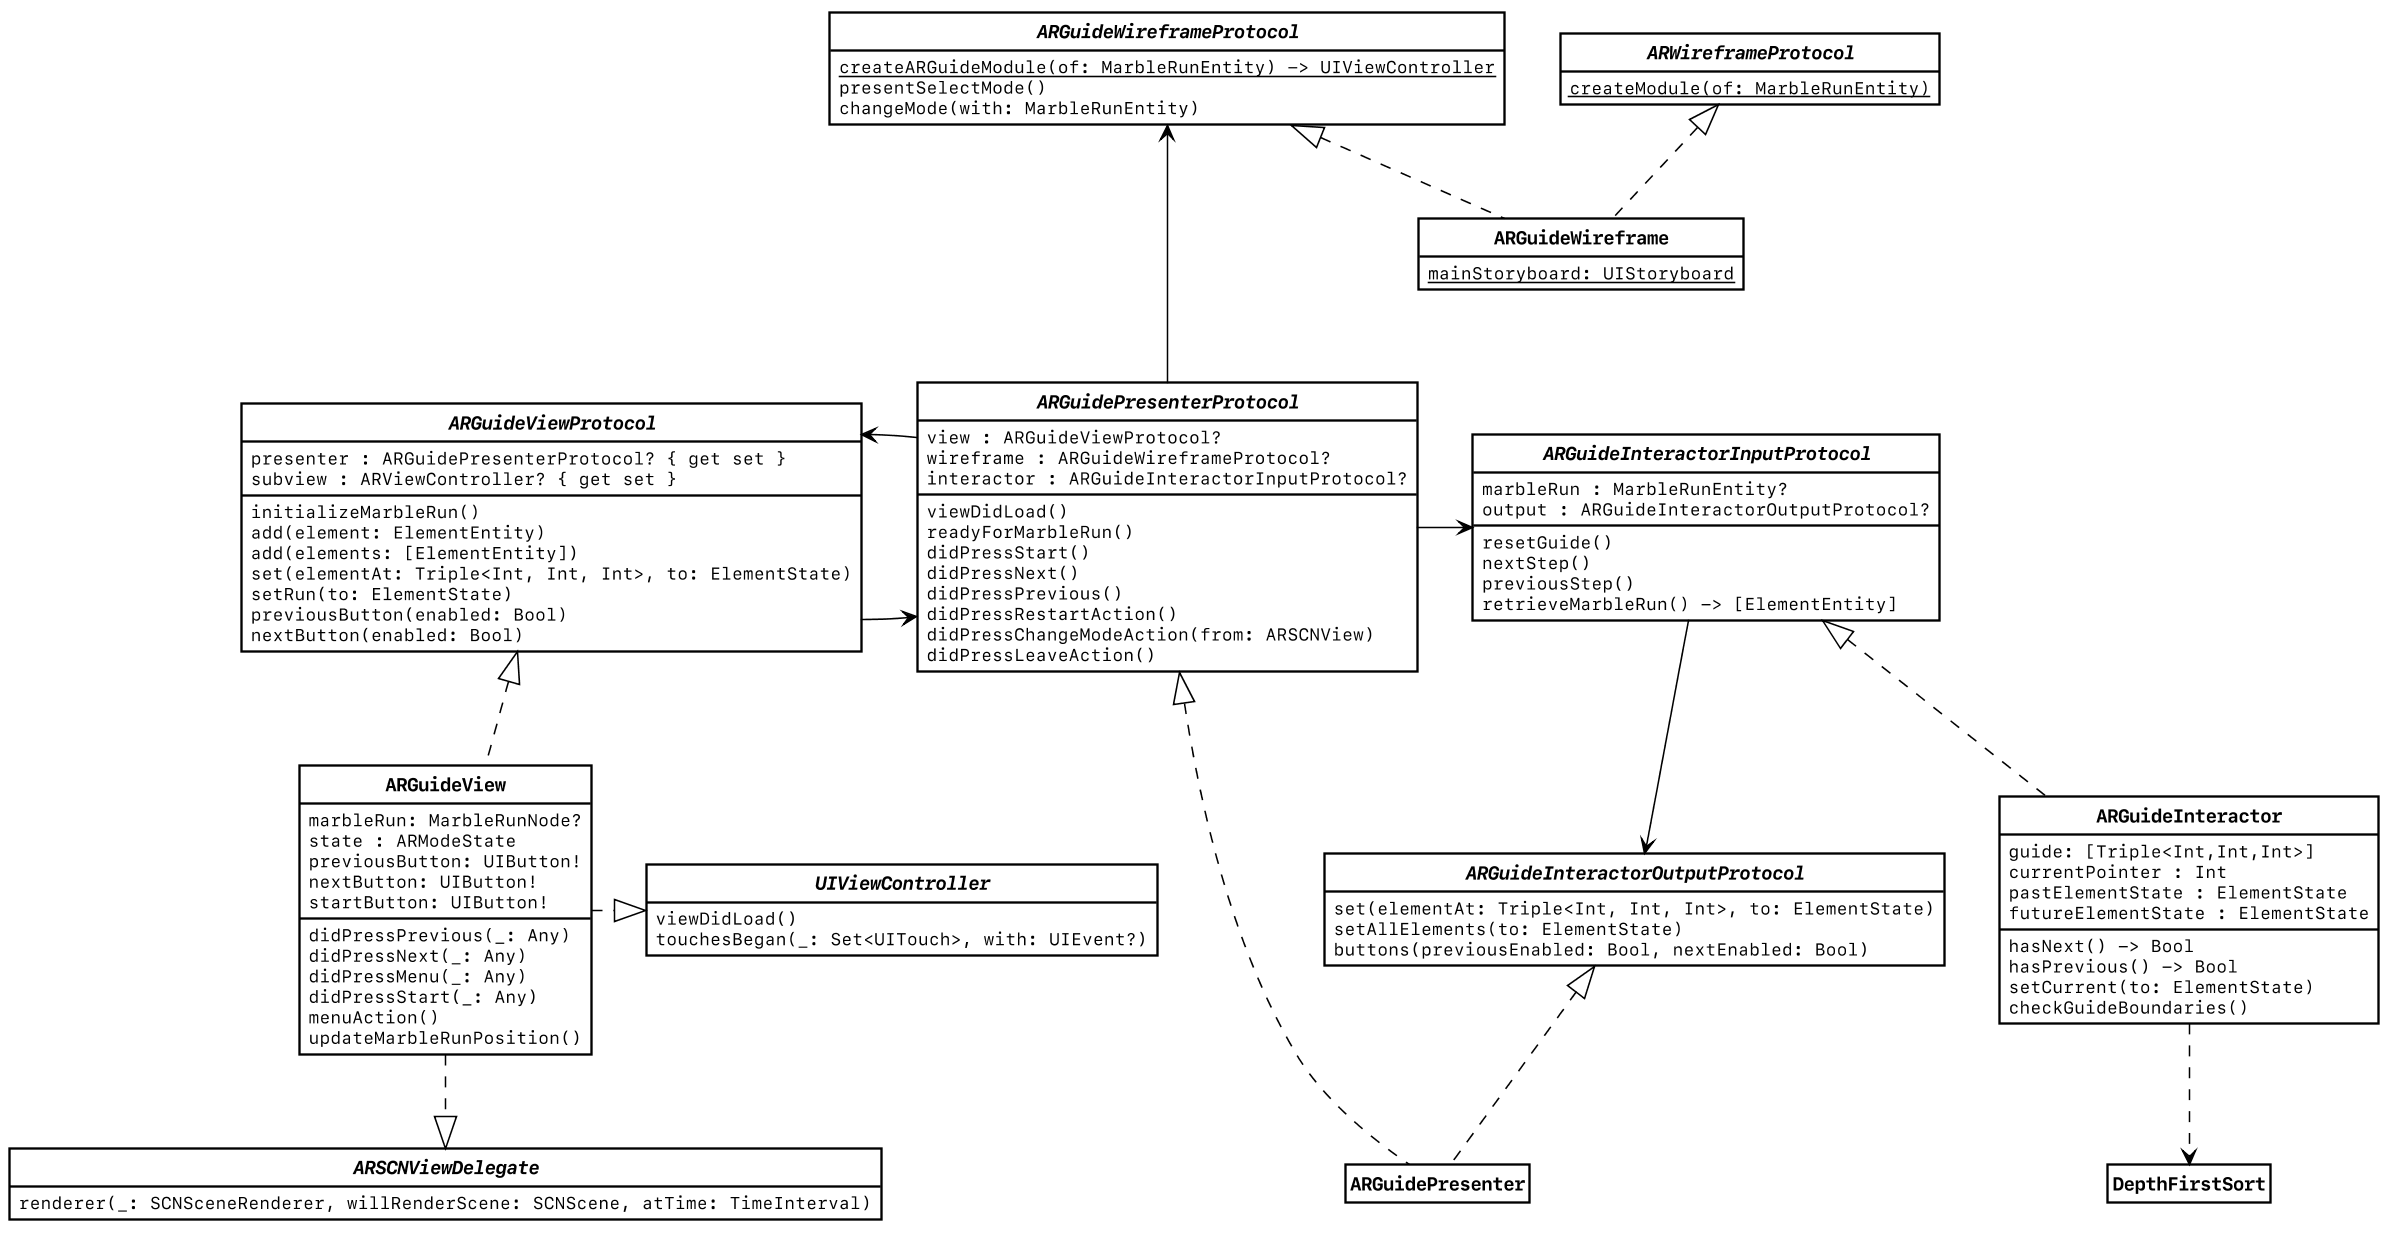
\includegraphics[width=1\textwidth]{classes-arguide}%
	\caption{Klassendiagramm des Moduls "`AR Guide"'}%
	\label{fig:classes-arguide}%
\end{figure}

Das Initialisieren der \texttt{SceneView} und des AR World Tracking übernimmt der \texttt{ARViewController} (siehe \ref{subsub:umsetzung-arviewcontroller}).
Sobald der Benutzer eine erkannte Fläche gewählt hat, übernimmt die \texttt{ARGuideView} die weiteren Aktionen und teilt dem Presenter mit, dass sie bereits ist, die Kugelbahn darzustellen.
Der Presenter fragt vom Interactor die Elemente der Kugelbahn an und fügt sie der View zu.
In \texttt{InitializeMarbleRun} der View wird eine \texttt{MarbleRunNode} erstellt und der Szene hinzugefügt, Elemente werden dann als Kindknoten der Kugelbahn ergänzt.
Die Positionierung der Kugelbahn erfolgt nach dem in Prototyp \ref{subsub:prot-kugelbahn} erarbeiteten Prinzip.

Ist die Position der Kugelbahn fixiert und der Startbutton wird gedrückt, lässt der Interactor von \texttt{DepthFirstSort} die Bauanleitung erstellen (siehe \ref{subsub:umsetzung-depthfirst}).
Der Rückgabewert ist ein Array von Koordinaten, in der Reihenfolgen, in der sie abgearbeitet werden sollen.
Mittels Vor- und Zurück-Buttons kann der Benutzer in der Anleitung navigieren.
Diese Aktionen erhöhen oder verringern im Interactor den \texttt{currentPointer}, der auf die aktuelle aktive Koordinate im Array \texttt{guide} zeigt.

Die View hat keine Kenntnisse über die Anleitung, sondern erhält als Reaktion auf Benutzerinteraktionen vom Presenter mit der Methode \texttt{set(elementAt:to:)} Anweisungen, welche Elemente der Kugelbahn welchen Status erhalten sollen.
So wird beispielsweise das aktive Element der Bauanleitung mit \texttt{ElementState.highlighted} hervorgehoben.

Als einziges Modul in diesem Projekt, nutzt der AR Editor für den Interactor ein Eingabe und Ausgabe Protokoll.
Während das \texttt{ARGuideInteractorInputProtocol} wie bei anderen Modulen vom Presenter genutzt wird um den Interactor anzusprechen, ist \texttt{ARGuideInteractorOutputProtocol} für die umgekehrte Richtung zuständig.

% TODO: Menu Action?

\subsubsection{AR Editor}

Im \texttt{AREditor} Modul wird die gewählte Kugelbahn in Augmented Reality bearbeitbar gemacht.
Abbildung \ref{fig:classes-areditor} zeigt das Klassendiagramm des Moduls.

Beim Laden der View werden die Gesten Tap, Long Press und Swipe mit den jeweiligen Eventhandler hinzugefügt.
Wie bei \texttt{ARGuide} übernimmt die Initialisierung der \texttt{SceneView} und von ARKit der \texttt{ARViewController}.
Auch die Positionierung der Kugelbahn läuft nach dem selben Muster.

Nachdem die Position der Kugelbahn fixiert wurde, kann der Editiermodus mit dem Startbutton gestartet werden.
Damit wird der \texttt{state} auf \texttt{ARModeState.editorMode} gesetzt.

\begin{figure}[htb!]
	\centering
	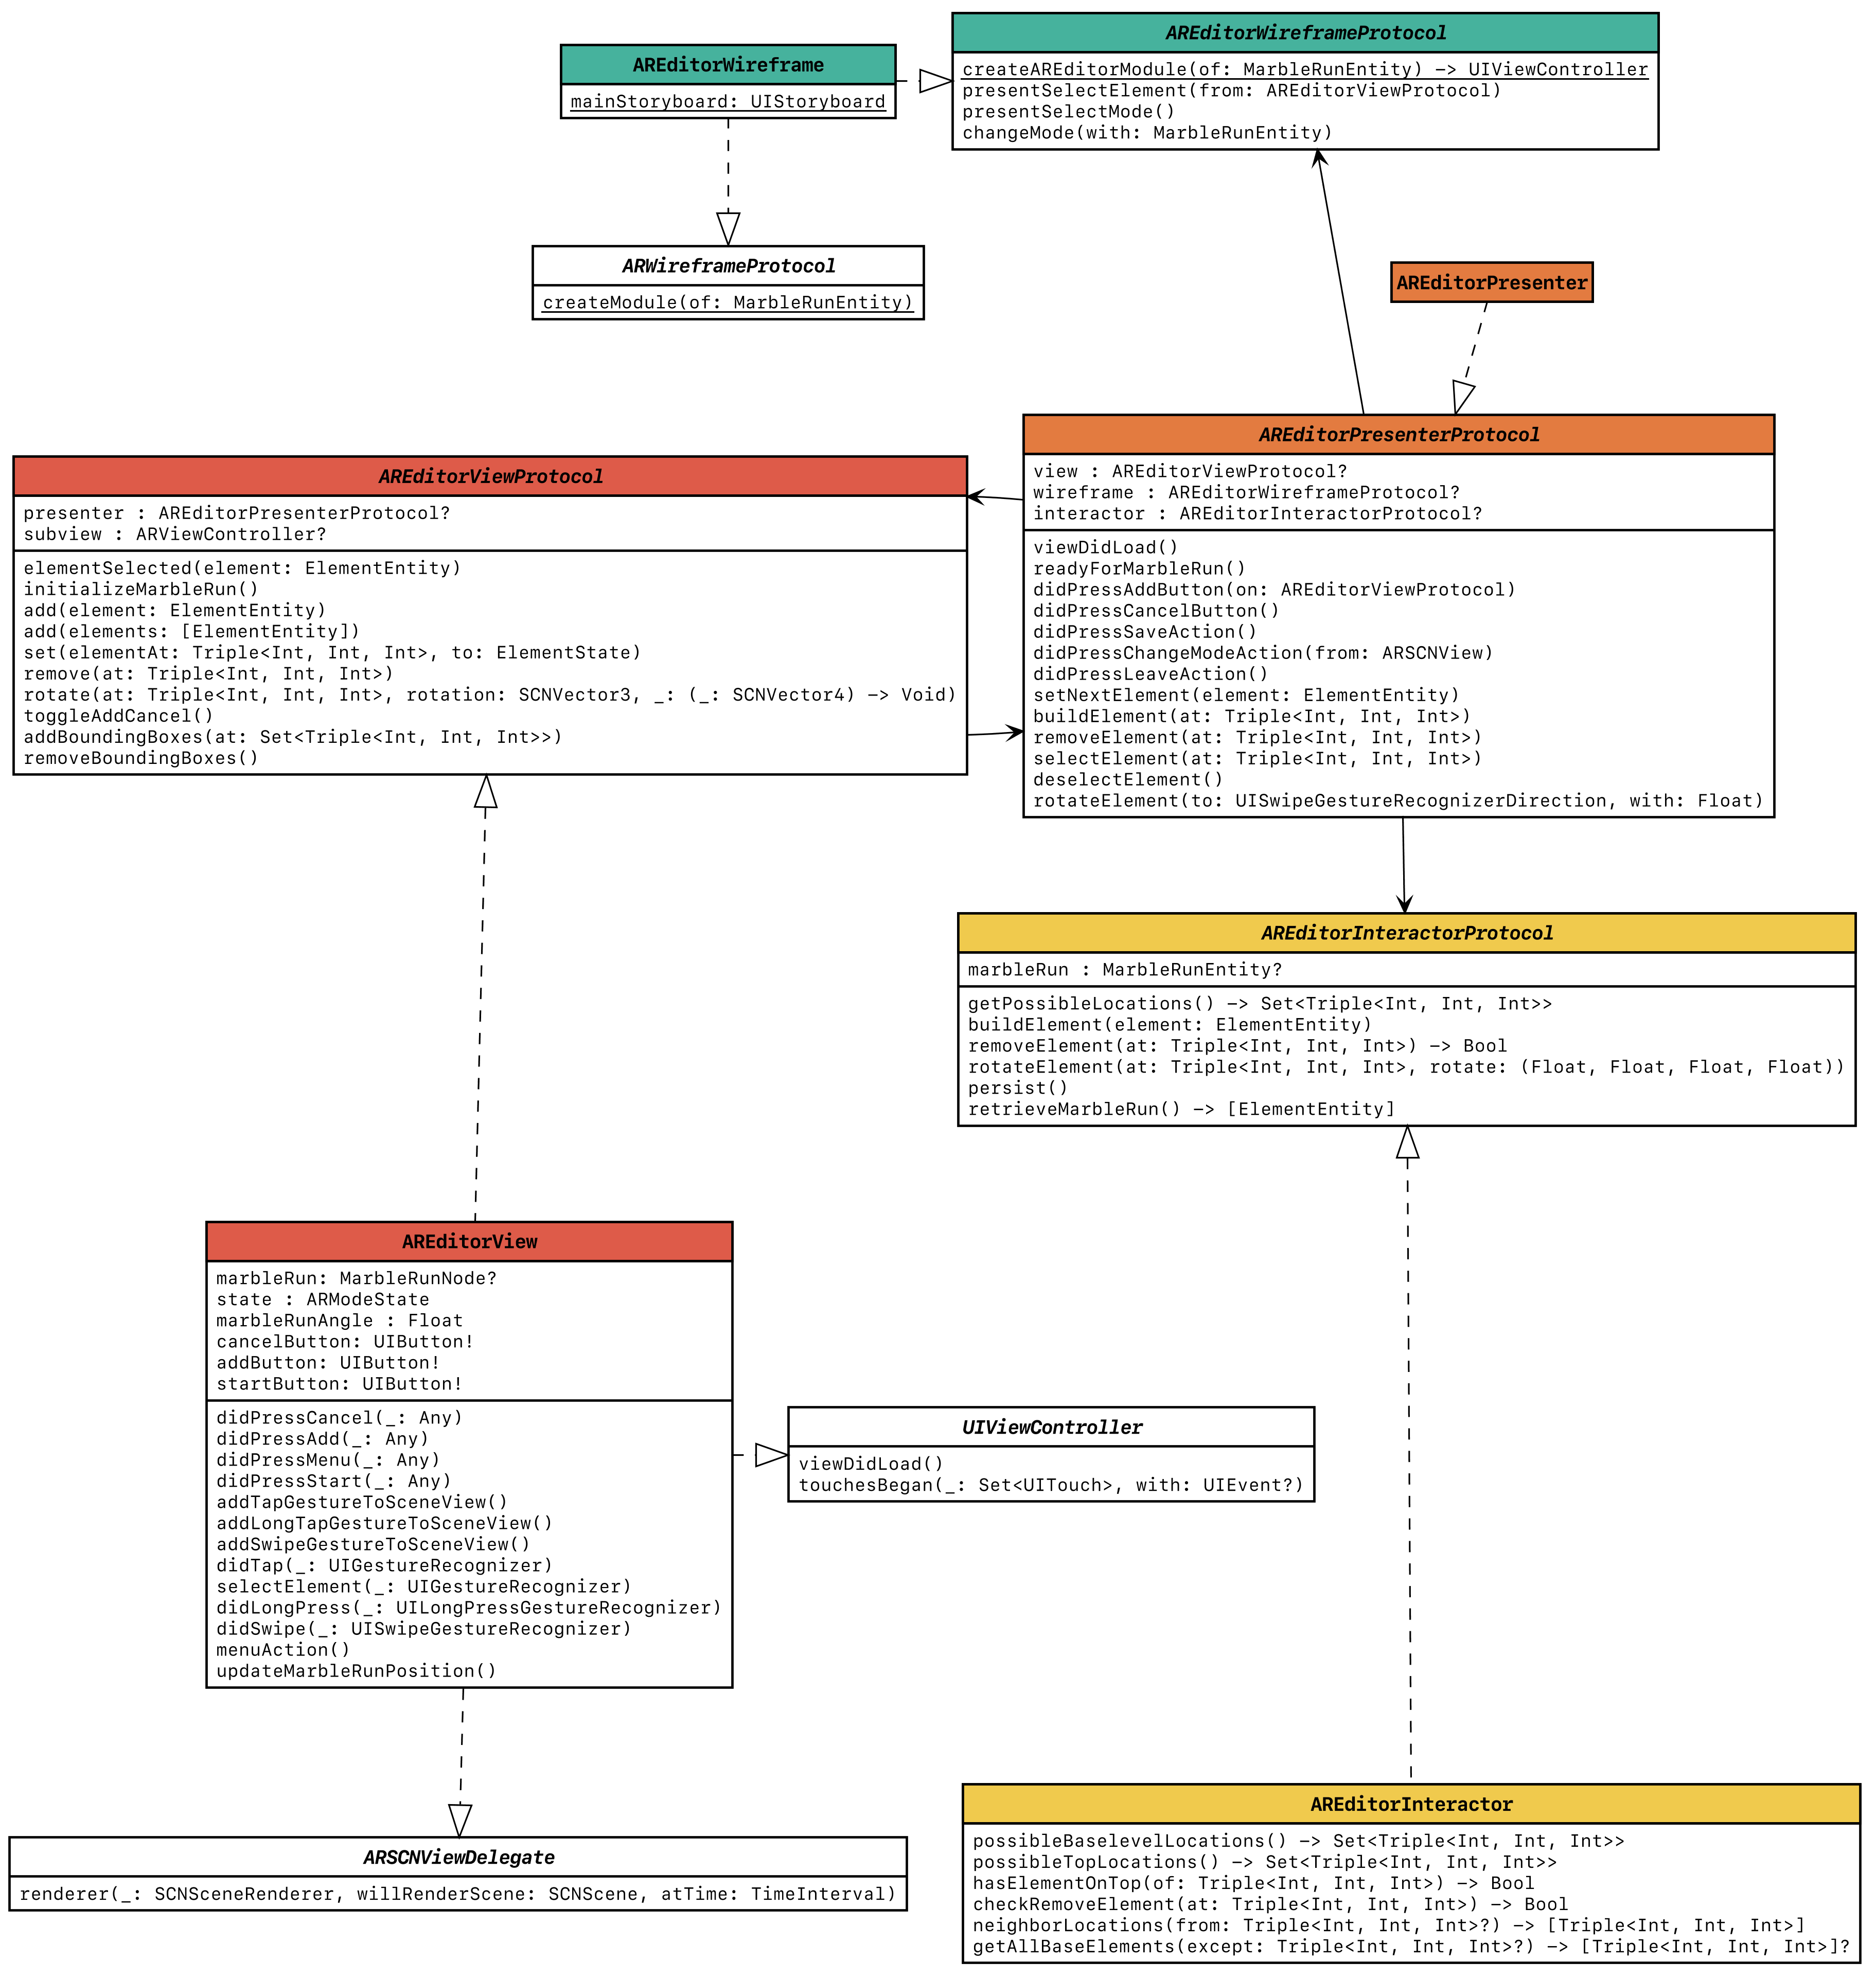
\includegraphics[width=1\textwidth]{classes-areditor}%
	\caption{Klassendiagramm des Moduls "`AR Editor"'}%
	\label{fig:classes-areditor}%
\end{figure}

\textbf{Neues Element hinzufügen} \\
Bei einem Druck des \texttt{addButton} wird das Modul \texttt{ElementList} aufgerufen, von dem die View schliesslich den selektierte Elementtyp durch die Methode \texttt{elementSelected(element:)} erhält.
Dem Presenter wird diese Information weitergeben und dieser fragt beim Interactor nach den möglichen Positionen, an denen das Element platziert werden kann.
Der Interactor sucht einerseits nach allen Koordinaten auf der untersten Ebene der Kugelbahn, die an ein existierendes Element angrenzen und noch leer sind (Methode \texttt{possibleBaselevelLocations()}).
Andererseits wird in \texttt{possibleTopLocations()} nach Elementen gesucht, auf denen noch kein Element steht.
Diese Kriterien führen dazu, dass die Bahn physikalisch möglich ist (keine schwebeden Elemente) und zusammenhängend ist (nur angrenzende Positionen).

All diese Positionen werden als \texttt{BoundingBoxNode} der View hinzugefügt und dargestellt.
Tippt der Benutzer auf einer der Boxen, wird diese mit dem zuvor gewählten Elementtyp ersetzt und alle anderen Positions-Boxen werden wieder ausgeblendet.
Der Presenter gibt dabei die \texttt{ElementEntity} mit aktualisierten Koordination sowohl an den Interactor als auch an die View.

\textbf{Element löschen} \\
Die Methode \texttt{didLongPress(\_:)} macht auf die SceneKit Szene einen Hittest.
Wenn das Resultat des Hittests ein Kugelbahn Element ist, wird beim Presenter die Methode \texttt{removeElement(at:)} aufgerufen.
Damit wird versucht das entsprechende Element beim Interactor zu entfernen.
Der Interactor überprüft in der Methode \texttt{removeElement(at:)}, ob das Element überhaupt entfernt werden darf.
Dazu darf sich als erstes kein Element darüber befinden.

Wenn sich das Element auf der untersten Ebene der Kugelbahn befindet, dürfen mit dessen Löschung auch keine "`Inseln"' entstehen, sprich die Kugelbahn soll zusammenhängend bleiben.
Das wird in \texttt{checkRemoveElement(at:)} überprüft, indem ausgehend von einem beliebigen Element eine Tiefensuche via direkte Nachbarschaften durchgeführt wird.
Das zu entfernende Element wird dabei ausgelassen.
So werden angrenzende Elemente so lange zur Liste der besuchten Elemente hinzugefügt, bis keines mehr gefunden wird, das nicht bereits besucht wurde.
Eine durch die Löschung entstehende Lücke führt dazu, dass nicht alle Elemente der untersten Ebene besucht werden können.
Deshalb wird am Ende die Anzahl besuchter Elemente mit der Gesamtzahl der verbleibenden Elemente in der untersten Ebene verglichen.
Sind die beiden Zahlen unterschiedlich, hängt die Kugelbahn nach Entfernung des Elements nicht mehr zusammen und der Interactor gibt ein \texttt{false} an den Presenter zurück, der die Löschung abbricht.

\textbf{Element rotieren} \\
Wird ein Element durch Antippen ausgewählt, wird es hervorgehoben und der Presenter merkt es sich als \texttt{selectedElement}.
Ist das Attribut gesetzt und eine Swipe Geste wird ausgeführt, wird das Element in Richtung der Geste rotiert.
Die View berechnet den Winkel zwischen Kamera und Ausrichtung der Kugelbahn und gibt diesen zusammen mit der Richtung der Geste an die Presenter Methode \texttt{rotateElement(to:with:)}.
Es wird je nach Swipe-Richtung ein Vektor erstellt, der die Achse und Richtung der Rotation beschreibt.
Für einen Swipe nach links ist dies beispielsweise der Vektor \texttt{SCNVector3(0, -1, 0)} zur Rotation um die y-Achse.
Die korrekte Achse für vertikale Swipes ist abhängig vom Betrachtungswinkel.
Daher wird dort anhand des erhaltenen Winkels entweder die x- oder z-Achse mit einem positiven (1) oder negativen (-1) Wert belegt.

Ist die Rotation berechnet, wird der \texttt{rotation} Vektor in der View genutzt um auf dem ausgewählten Element eine Rotations-Aktion auszuführen, die wie folgt definiert wird:
\mint[style=xcode,breaklines]{swift}{let action = SCNAction.rotate(by: .pi/2, around: rotation, duration: 0.2)}
So wird das Element innert 0.2 Sekunden um 90° um die im Vektor definierte Achse rotiert.
Dabei bleibt das Koordinatensystem erhalten.

Das in Prototyp \ref{subsub:prot-interagieren} erarbeitete Vorgehen mit \texttt{SCNAction.rotateBy(x:y:z:rotation:)} und dem Zurücksetzen der Orientierung mit \texttt{SCNQuaternion}, erwies sich als Trick, der für die Demo-App nicht verwendet werden konnte.
Für einen Würfel, dessen Seiten alle gleich sind, funktioniert das Vorgehen zwar.
Aber die hier verwendeten Elemente zeigten, dass sich der Würfel nach der Rotation jeweils in den Originalzustand zurück versetzt. 

\subsubsection{Element List}

Das \texttt{ElementList} Modul listet alle verfügbaren Elementtypen auf, die der aktuell bearbeiteten Kugelbahn hinzugefügt werden können.
Es ist ähnlich dem \texttt{MarbleRunList} Modul.
Abbildung \ref{fig:classes-elementlist} zeigt das Klassendiagramm des Moduls.

\bild{1}{classes-elementlist}{Klassendiagramm des Moduls "`Element List"'}

Die \texttt{ElementListView} wird modal vom AR Editor dargestellt.
Sie meldet ihre Bereitschaft an den Presenter, der vom Interactor die Liste der Elementtypen abfragt.
Der Interactor greift dann wie folgt auf die SceneKit Scene mit den cuboro Elementen zu:
\mint[style=xcode,breaklines]{swift}{let cubes = SCNScene(named: "art.scnassets/cuboro-set.scn")?.rootNode}
Aus den Kindknoten von \texttt{cubes} stellt der Interactor ein Array von \texttt{ElementEntity} zusammen und gibt es als Rückgabewert dem Presenter zurück.
Dies wird an die View weitergegeben, welche daraus wie \texttt{MarbleRunList} ihre Collection View aufbaut.

Bei der Wahl eines Elementtyps durch den Benutzer ruft die View \texttt{didSelect(element:on:)} beim Presenter auf, was dieser an das Wireframe weitergibt.
Das Wireframe lässt die View ausblenden und gibt das selektierte Element an den AR Editor weiter.

\subsection{Persistenz}

\subsubsection{Data Manager} \label{subsub:umsetzung-datamanager}

Der Data Manager übernimmt das Lesen und Schreiben von persistierten, bzw. zu persistierenden Daten.
In dieser Demo-App sind dies die Kugelbahnen, bestehend aus einer \texttt{MarbleRunEntity} und ihrer \texttt{ElementEntity}s.
Der \texttt{MarbleRunDataManager} bietet statische Methoden zum Lesen aller Kugelbahnen (\texttt{retrieveMarbleRunList()}), Schreiben einer Kugelbahn (\texttt{persist(\_:)}) und einer Überprüfung, ob überhaupt gespeicherte Kugelbahnen vorhanden sind (\texttt{isDirectoryEmpty()}).

Als Dateiablage wird der Dokumentenordner des iOS Dateisystem mittels \texttt{FileManager} genutzt.
Die \texttt{MarbleRunEntity} jeder Kugelbahn wird mittels \texttt{NSKeyedArchiver} in einer eigenen Datei gespeichert:
\mint[style=xcode,breaklines]{swift}{NSKeyedArchiver.archiveRootObject(run, toFile: filePath.path)}
Damit dies möglich ist, müssen die Entitäten von \texttt{NSObject} erben und das \texttt{NSCoding} Protokoll adoptieren (Kapitel \ref{subsub:umsetzung-entities-nodes}).

\subsubsection{Entitäten und Nodes} \label{subsub:umsetzung-entities-nodes}

Die beiden zentralen Datenobjekte im Projekt sind Kugelbahnen und deren Elemente.
Sie werden für die Darstellung in der AR Szene aber auch zur Persistierung im Dateisystem gebraucht.
Aufgrund der VIPER Architektur wurden diese beiden Aspekte auch entsprechend getrennt.
Einerseits gibt es die \textbf{Nodes}, die von \texttt{SCNNode} erben und Informationen zur Geometrie und Erscheinungsbild haben.
Sie werden daher nur in den Views von AR Guide und AR Editor verwendet.
Anderersetis sind die \textbf{Entities} schlanke Klassen, die im Rest der App genutzt werden und persistiert werden können.

\textbf{Nodes} \\
Alle Nodes erben von der Klasse \texttt{SCNNode} und können so direkt in SceneKit verwendet und dargestellt werden.

\begin{description}
	\item[PlaneNode] ist zur Darstellung von durch ARKit erkannten Flächen. Sie hat eine \texttt{update} Methode, damit sie bei Änderungen der Grösse und Position aktualisiert werden kann.
	\item[BoundingBoxNode] ist ein einfacher Würfel, wie er als \texttt{BasicCube} in verschiedenen Prototypen verwendet wurde. Objekte dieses Typs werden im AR Editor zur Anzeige möglicher Positionen eines neuen Elements verwendet.
	\item[ElementNode] ist die Node für einzelne Kugelbahn Elemente. Sie hat eine \texttt{Triple} Location, einen Status vom Typ \texttt{ElementState} und einen Type, der ihre Geometrie definiert. Abhängig vom Status wird das Erscheinungsbild der Node verändert. Bei der Instanziierung wird basierend auf dem Type die Geometrie aus der SceneKit Scene "`cuboro-set.scn"' geladen. Die Position eines Elements wird mit \texttt{Triple} Koordinaten als relative Position zum Kugelbahn Ursprung in Anzahl Elemente definiert (\ref{subsub:umsetzung-triple}). Die reale Position wird durch die Multiplikation mit der Seitenlänge der Elemente berechnet.
	\item[MarbleRunNode] dient als Basisnode, der \texttt{ElementNode} Objekte hinzugefügt werden. Sie bietet Methoden, um sich mit \texttt{SCNBillboardConstraint} stets zur Kamera auszurichten, wie in Prototyp \ref{subsub:prot-kugelbahn} und Code \ref{code:prot-kugelbahn-billboardconstraint} gezeigt.
\end{description}

\textbf{Entities} \\
Die beiden Entitäten \texttt{MarbleRunEntity} und \texttt{ElementEntity} adoptieren das \texttt{NSCoding} Protokoll, um sie im Dateisystem zu persistieren.
Das Protokoll verlangt zwei Methoden – \texttt{init?(coder:)} und \texttt{encode(with:)} – in denen alle zu persistierenden Attribute kodiert, beziehungsweise dekodiert, werden müssen.


\subsection{Storyboard}

Abbildung \ref{fig:project-storyboard} zeigt das Storyboard des Projekts.

\bild{1}{project-storyboard}{Das Storyboard des Projekts}


\subsection{Weitere Bestandteile}

\subsubsection{Triple} \label{subsub:umsetzung-triple}
Das Struct Triple beinhaltet ein Tupel mit drei Elemente. Tripel adoptiert das Hashable Protokoll um auch im Set verfügbar zu sein.

Das Triple wird dazu verwendet die relativen Koordinaten der Kugelbahn Elemente festzuhalten. Anhand dieser Koordinaten können Berechnungen zwischen den Elementen durchgeführt werden wie z.B. Die benachbarten Elemente gefunden werden.

\subsubsection{Enums} \label{subsub:umsetzung-enums}

Über \texttt{ARModeState}, \texttt{ARInteractionMode}

\subsubsection{DepthFirstSort} \label{subsub:umsetzung-depthfirst}

\subsubsection{ARViewController} \label{subsub:umsetzung-arviewcontroller}

\subsubsection{Initializer}

\subsubsection{Informationsbildschirm}
Oben rechts auf dem Startbildschirm befindet sich ein Informationsicon mit dem der Informationsbildschirm eingeblendet werden kann. Dieser zeigt die aktuelle Version, Entwickler, Abhängigkeiten und dass die App als Resultat der Industrieprojektarbeit an der Fachhochschule Luzern entstanden ist. Zusätzlich kann der Debug Modus aktiviert werden um Laufzeitinformationen der AR View zu erhalten. Ob der Debug Modus aktiviert ist, wird in den User Defaults gespeichert.

}

\IfFileExists{10-Validierung}{
  \section{Validierung}


\subsection{Funktionale Anforderungen}

Die detaillierten funktionalen Anforderungen sind im Kapitel \ref{appendix:user-stories} aufgeführt.

\begin{longtable}{l l p{10cm} l}
	\hline
	\textbf{Nr.} & \textbf{Prio.} & \textbf{Beschreibung} & \textbf{Status} \\
	\hline
	\textbf{1} & & \textbf{Allgemein} & \\
	\hline
	1.1 & M & Die erkannte Fläche wird mit einem augmentierten Gitternetz angezeigt. Durch Antippen der Fläche wird diese ausgewählt. Die Position der neu zu setzenden Kugelbahn orientiert sich an der ausgewählten Fläche. & Erfüllt \\
	\hline
	1.2 & M & Die Kugelbahn wird auf der ausgewählten Fläche angezeigt. Die Kugelbahn befindet sich zentral im Kamerabild. Mit einem Tap kann die Bahn fixiert werden. & Erfüllt \\
	\hline
	1.3 & M & Die Bahn ist parallel zur Kamera ausgerichtet und behält dies auch beim drehen des Gerätes bei. & Erfüllt \\
	\hline
	1.4 & M & Auf der AR View wird oben links in schwarzer Schrift der aktuelle Modus visualisiert. & Erfüllt \\
	\hline
	1.5 & S & Diese Funktionalität wurde nicht implementiert. Als möglicher Workaround kann der Modus neu gestartet werden. & Nicht Erfüllt \\
	\hline
	1.6 & K & Der Modus kann direkt im Menu gewechselt werden. Beim Wechsel bleibt die aktuelle Szene nicht bestehen und muss somit neu ausgerichtet werden. & Teilweise Erfüllt \\
	\hline
	\textbf{2} & & \textbf{Guide} & \\
	\hline
	2.1 & M & Alle persistierten Bahnen werden mit dem Namen der Kugelbahn in der View MarbleRuns visualisiert. Diese Bahnen können durch Antippen ausgewählt werden. Nach erfolgreicher auswahl einer Bahn wird diese der AR View bereitgestellt. & Erfüllt \\
	\hline
	2.2 & M & Beim Aufbau der Bahn wird das nächte physisch zu platzierende Element rot transparent angezeigt. Die restlichen Elemente sind weiss transparent ersichtlich. Anhand der transparenten Darstellung wird hervorgehoben, welches Element für den Aufbau verwendet werden muss und in welcher Position es sich befinden soll.  & Erfüllt \\
	\hline
	2.3 & M & Falls ein nächster Schritt in der Bauanleitung zur Verfügung stehen, ist auf der AR View unten rechts ein oranger Button mit einem Pfeil nach rechts verfügbar. Mit diesem Button kann der nächste Schritt angezeigt werden. Sollte ein nächster Schritt verfügbar sein, so wird der Button ausgegraut. & Erfüllt \\
	\hline
	2.4 & S & Falls ein vorheriger Schritt in der Bauanleitung zur Verfügung steht, ist auf der AR View unten links ein oranger Button mit einem Pfeil nach links verfügbar. Mit diesem Button kann der vorherige Schritt angezeigt werden. Sollte kein vorheriger Schritt verfügbar sein, so wird der Button ausgegraut. & Erfüllt \\
	\hline
	2.5 & K & Die Bauanleitung kann über das Menu oben rechts neu gestartet werden. Zuoberst im Menu befindet sich der Button unter "'Restart Guide`"'. & Erfüllt \\
	\hline
	\textbf{3} & & \textbf{Builder} & \\
	\hline
	3.1 & M & Zur Auswahl stehen 13 cuboro Elemente. Diese können mit dem grünen Plus-Button in der unteren Mitte selektiert werden. & Erfüllt \\
	\hline
	3.2 & M & Wird auf dem Startbildschirm der Editor-Modus ausgewählt so wird eine Liste der persistierten Bahnen angezeigt. Das erste Element dieser Liste ist ein Plus, bei dem eine neue Bahn erstellt werden kann. Beim erstellen einer neuen Bahn wird der Namen der Bahn mit einem Popover eingegeben. Die neue Bahn wird unter dem eingegeben Namen persistiert und steht ab diesem Zeitpunkt in der Liste zur Verfügung. & Erfüllt \\
	\hline
	3.3 & M & Nach dem bearbeiten einer Kugelbahn, kann diese über das Menu oben links persistiert werden. Dies geschieht über den Button "'Save`". & Erfüllt \\
	\hline
	3.4 & M & In der MarbleRuns-Liste kann eine persistierte Bahn ausgewählt werden. Diese steht anschliessend zur Positionierung in der AR View zur Verfügung. Sobald die Bahn platziert wurde, kann sie beliebig verändert werden. & Erfüllt \\
	\hline
	3.5 & M & Valide Positionen werden nach der Selektion eines Elementes auf der Kugelbahn als Bounding Box dargestellt. Die Bounding Boxen werden mit einem Algorithmus nur an Positionen angezeigt, die auf der ersten Ebene, direkt an einem bereits erstellten Element, angrenzen oder darauf platziert werden kann. & Erfüllt \\
	\hline
	3.6 & M & Mit dem Antippen einer Bounding Box wird ein Element an der jeweiligen Stelle hinzugefügt. Es ist nur möglich Elemente an den Stellen einer Bounding Box hinzuzufügen. & Erfüllt \\
	\hline
	3.7 & M & Durch das Antippen von einem Element kann dieses selektiert werden. Bei erfolgreicher Selektion, wird dieses rot transparent hervorgehoben. Anschliessend kann das Element durch Streichgesten in einer der drei Achsen in richtung der Geste um 90° rotiert werden. & Erfüllt \\
	\hline
	3.8 & M & Durch das Antippen und halten kann ein Element entfernt werden. Dies kann jedoch nur gemacht werden, wenn die Kugelbahn zusammenhängend bleibt und physikalisch möglich ist. Es ist somit nicht möglich Elemente unterhalb von Elementen zu entfernen (keine schwebende Elemente). & Erfüllt \\
	\hline
	3.9 & S & Diese Funktionalität ist nicht implementiert, da die zeitlichen Aufwände anderweitig investiert werden mussten. & Nicht Erfüllt \\
	\hline
	\caption{Validierung der funktionalen Anforderungen}
\end{longtable}


\subsection{Nichtfunktionale Anforderungen}


Die detaillierten nichtfunktionale Anforderungen sind im Kapitel \ref{appendix:nichtfunktionale-anforderungen} aufgeführt.

\begin{longtable}{l l l p{10cm}}
	\hline
	\textbf{Nr.} & \textbf{Prio.} & \textbf{Typ} & \textbf{Beschreibung} \\
	\hline
	 & & \textbf{Constraints} & \\
	\hline
	01 & M & Technologie & Die App wurde in Swift 4.1 programmiert. \\
	\hline
	02 & M & Technologie & Die App wurde auf den iPhones 6s und 7 mit iOS 11.3 getestet. \\
	\hline
	03 & M & Technologie & Die App wurde mit ARKit 1.5 entwickelt. \\
	\hline
	04 & M & Geschäftlich & Die App zeigt die technologischen Möglichkeiten auf. \\
	\hline
	 & & \textbf{Qualitäten}& \\
	\hline
	05 & M & Laufzeit & Farben wurden nur unterstützend verwendet. Die Interaktionen sind unmissverständlich mit Symbolen oder Beschriftung versehen. \\ 
	\hline
	06 & M & Laufzeit & Der Benutzer wird aktuell nicht über den aktuellen Trackingstatus informiert. \\
	\hline
	07 & M & Laufzeit & Die Bildwiederholungsfrequenz mit 30 Bilder pro Sekunde kann bei 20 Elementen garantiert werden und wurde getestet. \\
	\hline
	08 & M & Laufzeit & Die Persistierung der Kugelbahnen erfolgt auf dem Gerät. \\
	\hline
	09 & M & Compilier-Zeit & Der Code wurde möglichst klar und sauber geschrieben. \\
	\hline
	10 & M & Compilier-Zeit & Schlüsselstellen im Code sind in der Dokumentation festgehalten. Zusätzlich wurde sporadisch auf kurze Kommentare zurückgegriffen, die bei einer Code passage erklären was passiert. \\
	\hline
	\caption{Validierung der nichtfunktionalen Anforderungen}
\end{longtable}


\subsection{Technisches Fazit}
Bei der Umsetzung der App wurde zuerst die Architektur diskutiert und erstellt. Dies hat anfangs zwar Zeit gekostet, konnte aber im Verlauf des Projektes seinen Mehrwert präsentieren. Die VIPER Architektur hat mit seiner losen Koppelung und klaren Modularisierung überzeugt. Diese Modularisierung verhilft ein schnelles einarbeiten in das Projekt und eine einfache Möglichkeit dieses um neue Funktionalitäten zu erweitern. Der Editiermodus zur Erstellung und Modifikation, sowie die interaktive Aufbauanleitung von virtuellen Kugelbahnen konnte realisiert werden.

% AR Experience wird unterbrochen
Bei der Auswahl des nächsten Elements für die virtuelle Kugelbahn wird das AR Erlebnis unterbrochen. Hierbei benötigt das Framework einige Sekunden die Bahn wieder richtig zu Positionieren.

% Anforderungen eingehen
Die Erkennung dreidimensionaler Objekte mit den vorgeschlagenen Frameworks konnte nicht erfolgreich implementiert werden und wurde in der Umsetzung der Demo-App nicht weiter berücksichtigt. Die Demo-App erfüllt alle Muss-Anforderungen und enthält einen Baumodus sowie eine interaktive Aufbauanleitung.

}

\section{Schlussfolgerungen}
\subsection{Lessons Learned}
\subsection{Ausblick}


%----------------------------------------------------------------------------------------
%	Bibliography
%----------------------------------------------------------------------------------------
\newpage
\section{Quellen und Verzeichnisse}
\bibliographystyle{apacite}
\bibliography{Quellen}
%------------------------------------------------
\newpage
%\section{Abbildungsverzeichnis}
\listoffigures
\addtocontents{lof}{\protect\thispagestyle{headings}}
%------------------------------------------------
\newpage
%\section{Tabellenverzeichnis}
\listoftables
\addtocontents{lot}{\protect\thispagestyle{headings}}
%------------------------------------------------
\newpage
%\section{Codeverzeichnis}
\listoflistings
\addtocontents{lol}{\protect\thispagestyle{headings}}


%----------------------------------------------------------------------------------------
%	Appendix
%----------------------------------------------------------------------------------------
\newpage
\pagestyle{headings}
\appendix
\setcounter{figure}{0}
\setcounter{table}{0}
\renewcommand{\thefigure}{\thesection\arabic{figure}}
\renewcommand{\thetable}{\thesection\arabic{table}}
\renewcommand{\thesubsection}{\thesection\arabic{subsection}}


\IfFileExists{90-Appendix}{
  \section{Projektmanagement}

\subsection{Aufgabenstellung}
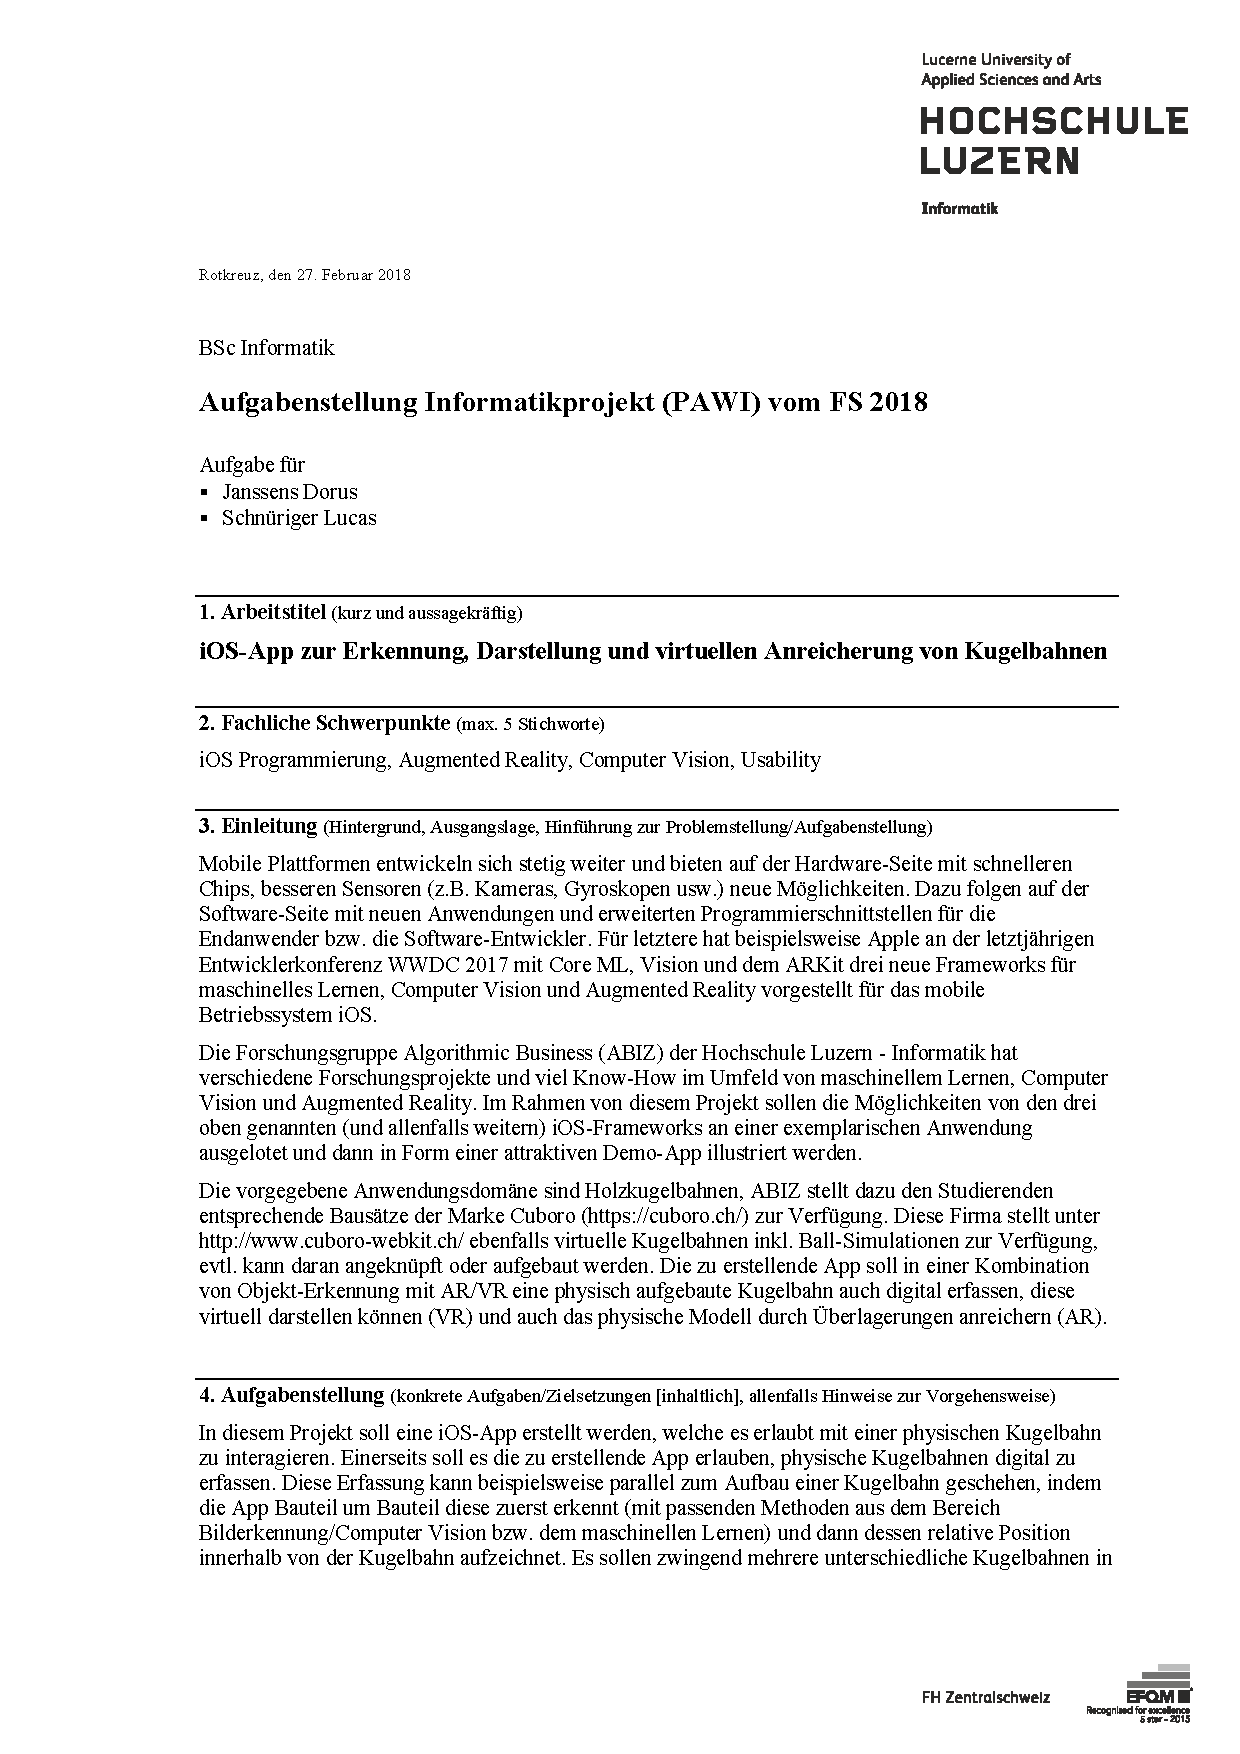
\includepdf[pages=-]{appendix/Aufgabenstellung_PAWI_FS_2018_Janssens_Schnueriger.pdf}

\IfFileExists{99-Risikomanagement}{
	\newpage
	\subsection{Risikomanagement}

\begin{longtable}{lp{3.5cm}lllp{3.5cm}p{3.5cm}}
	\hline
	\textbf{Nr.} & \textbf{Beschreibung} & \textbf{W} & \textbf{A} & \textbf{W*A} & \textbf{Prävention} & \textbf{Reaktion} \\ 
	\hline
	01  & Ausfall eines Projektmitarbeiters & 1 & 2 & 2 & Regelmässiger Wissensaustausch und Projektmeetings, zentrale Dokumentation aller Vorgänge (GitHub) & Betreuenden Dozenten informieren und Anforderungen einschränken \\
	\hline
	02  & Projektdaten gehen verloren & 0 & 3 & 0 & Daten regelmässig sichern, Daten versionisiert auf GitHub & Daten wiederherstellen \\
	\hline
	03  & GitHub fällt aus & 1 & 1 & 1 & lokale Kopien aller Daten & auf lokalen Kopien arbeiten und auf HSLU GitLab migrieren \\
	\hline
	04  & Anforderungen werden nicht erfüllt & 1 & 2 & 2 & regelmässiges Überprüfen / Meetings mit betreuendem Dozenten, realistische Ziele setzen & Rechtzeitige Information an Projektbeteiligte und Anpassung des Projektplans \\
	\hline
	05  & Zeitaufwand und Komplexität für Entwicklung zu hoch & 1 & 3 & 3 & eingehende Technologierecherche und Versuche & Betreuenden Dozenten informieren, um Hilfe bei Dozenten suchen, Anforderungen einschränken \\
	\hline
	06  & Frameworks weisen nicht die funktionalen Anforderungen auf die im Marketing versprochen werden. & 1 & 3 & 3 & Mittels Problemlösungszyklen die Funktionalität überprüfen und verifizieren & Rücksprache mit dem Auftraggeber und dem Betreuer \\
	\hline
	07  & Beschränkte Erfahrung mit iOS und Swift erhöht die Zeit der Evaluation und gefärdet somit den tiefe Grad der Problemlösungszyklen. & 1 & 3 & 3 & Genügend Zeit bei den ersten Problemlösungszyklen definieren & Anpassung der Anforderungen und Rücksprache mit dem Auftraggeber und dem Betreuer \\
	\hline
	08  & Betas von ARKit 1.5 oder iOS 11.3 sind instabil oder ändern genutzte Funktionen & 0 & 2 & 0 & Known Issues recherchieren, Verwendung von neuen Funktionen bewusst wählen und Alternativen berücksichtigen & Issue an Apple reporten, an anderen (gleich wichtigen) Aufgaben arbeiten, alternative Methoden suchen, auf stabile Funktionen zurückgreifen \\
	\hline
	09  & Leistung der (Test)Geräte nicht ausreichend & 1 & 2 & 2 & Technologische Anforderungen (welche Generation von iPhones/iPads) in der Recherche berücksichtigen, beim Bau von Prototypen Zeit einplanen zu Performance Tests & Code/Methoden optimieren, alternative Lösungen weiterverfolgen \\
	\hline
	10  & Präzision des Tracking zu niedrig um das Cuboro Element sicher zu Tracken & 2 & 2 & 4 & Anforderungen mit einem Tolleranzbereich definieren. & Marker anbringen um die präzision des Trackings zu erhöhen. Third party Software zur erkennung des Würfels verwenden. \\
	\hline
	11  & Präzision der Hit-Tests zu niedrig um zu ermitteln ob sich ein physisches Objekt in einer augmentierten Bounding Box befindet & 2 & 2 & 4 & Bestätigen mittels einer Tapgeste oder einem Button klick. & Verschiedene Versuche durchführen um die Genauigkeit zu ermitteln. \\
	\hline
	12  & Erhalten keine oder nicht verwendbar 3D Daten von cuboro Elemente & 1 & 2 & 2 & Kontakt mit cuboro herstellen & Einfache Würfel als Platzhalter, eigene einfache Elemente mit SceneKit oder Drittanbieter Software (bspw. Blender) erstellen \\
	\hline
	13  & Präzision des Worldtrackings ist zu instabil um die Bahn auf der ausgewählten Fläche zu halten & 2 & 2 & 4 & ARKit 1.5 nutzen & Funktion um die Bahm manuell zu korrigieren \\
	\hline
	14  & Korrekte Rotation der Elemente zu komplex & 2 & 2 & 4 & - & Anzahl Rotationsachsen verringern \\
	\hline
	15  & Worldtracking bei Unterbrüchen zu instabil & 2 & 2 & 4 & Unterbrüche der Szene vermeiden & Popup statt Modal verwenden um keinen Unterbruch zu erzeugen, Benutzer über Relokalisierung informieren \\
	\hline
\end{longtable}

\textbf{Legende}
\begin{itemize}
	\item \textbf{W:} Wahrscheinlichkeit
	\item \textbf{A:} Auswirkungen
\end{itemize}

\subsubsection*{Änderungsprotokoll}

\begin{table}
	\begin{tabular}{llp{10cm}}
		\hline
		\textbf{Datum} & \textbf{Autor} & \textbf{Bemerkungen} \\
		\hline
		06.03.2018 & Lucas & Erstellung der Tabelle mit Risiken 01-05 \\
		10.03.2018 & Dorus & Erweiterung um Risiken 06-07 \\
		12.03.2018 & Lucas & Erweiterung um Risiken 08-09 \\
		26.03.2018 & Lucas \& Dorus & Erweiterung um Risiko 10 \\
		26.03.2018 & Dorus & Risiko 07 W heruntergestuft von 2 auf 1 \\
		09.04.2018 & Dorus & Erweiterung um Risiko 11 \\
		09.04.2018 & Lucas & Risiko 08 W heruntergestuft von 1 auf 0, iOS 11.3 / ARKit 1.5 sind veröffentlicht \\
		22.04.2018 & Lucas & Erweiterung um Risiko 12 \\
		22.04.2018 & Lucas \& Dorus & Erweiterung um Risiko 13 \\
		07.05.2018 & Lucas & Risiko 10 heruntergestuft von 3 auf 2 \\
		07.05.2018 & Lucas & Risiko 12 heruntergestuft von 2 auf 1 \\
		21.05.2018 & Lucas \& Dorus & Erweiterung um Risiken 14-15 \\
		\hline
	\end{tabular}
\end{table}


}

\IfFileExists{99-Protokolle}{
	\newpage
	\subsection{Protokolle}

\setlist[itemize]{noitemsep}

\subsubsection*{22.05.2018 - Sitzung}

Anwesend: Ruedi Arnold, Lucas Schnüriger, Dorus Janssens

\textbf{Fragen}
\begin{itemize}
	\item Demo-App: Rotation um nur eine Achse auch akzeptabel?
	\begin{itemize}
		\item Noch einmal eine Stunde investieren, um zu sehen, ob die Rotation um alle drei Achsen nicht doch geht, bspw. mit einer Transformationsmatrix
	\end{itemize}
	\item Dokumentation:
	\begin{itemize}
		\item Wie sollen die (funktionalen) Anforderungen festgehalten werden: Teil des Hauptteil (Problemstellung) oder in Anhang (Architekturdokumentation)?
		\item Anforderungen können im Anhang gehandhabt werden. Sie sollen aber nicht doppelt aufgeführt werden.
	\end{itemize}
	\item Prototypen: die Fragestellungen und Resultate in einer Übersicht sammeln oder Teil der Prototypen Beschreibung oder gar an beiden Stellen?
	\begin{itemize}
		\item Kurze Liste mit Beschreib der Unterfangen, allenfalls Erfüllungsgrad visualisieren (bspw. mit Ampelsystem)
		\item Der bisherige Aufbau zur Beschreibung der Prototypen sonst ist ok
	\end{itemize}
	\item Umfang des Testing: Testplan und Testprotokoll oder einfach Anforderungen validieren? Wie dokumentieren: in Hauptteil/Anhang?
	\begin{itemize}
		\item Anforderungen validieren anhand der Akzeptanzkriterien, Erfüllungsgrad prüfen und Unvollständigkeiten begründen
		\item Festhalten im Hauptteil unter "Validierung" passt
		\item Unit Tests nicht notwendig
	\end{itemize}
\end{itemize}

\textbf{Weitere Arbeitsschritte / zu bearbeitende Fragestellungen}
\begin{itemize}
	\item Demo-App fertigstellen:
	\begin{itemize}
		\item Rotation nochmals überarbeiten und allenfalls darlegen warum es nicht funktioniert
		\item Löschalgorithmus fertig implementieren, sodass keine "Inseln" gebildet werden können
		\item Einen "About"-Bereich ergänzen (mit Name, Version)
		\item Das Schachbrettmuster der Flächenerkennung nach Start Editor/Guide nicht mehr anzeigen, oder transparenter
		\item Methoden der Klasse zur Persistierung statisch machen, nicht als Objekt benötigt
	\end{itemize}
	\item Dokumentation fertigstellen:
	\begin{itemize}
		\item Wichtig: Dokumentation muss eine objektive Bewertung und ein persönliches Fazit (pro Student) enthalten
		\item Die Projektplanung (Grobplan/Meilensteine) kann direkt in den Hauptteil der Dokumentation unter "Problemstellung"
		\item Protokolle, Arbeitsjournale, Risikomanagement im Anhang der Dokumentation mit abgeben aber nicht ausdrucken
		\item Aufgabestellung in den Anhang, Einleitung/Ausgangslage mit eigener Formulierung
		\item Source Dateien im Anhang (nicht nur von Prototypen/App, sondern auch von Bildern, Grafiken und Diagrammen)
		\item Den Backlog wenn möglich anhängen (vom GitHub Project nach Möglichkeit exportieren)
	\end{itemize}
	\item Demo Video erstellen
\end{itemize}

\textbf{Varia}
\begin{itemize}
	\item Zum letzten Statusprotokoll: der 1. und 3. Arbeitsschritt aus "Stand der Arbeit" würde in "Ausgeführte Arbeiten" kommen, "Stand der Arbeit" sollte SOLL-IST vergleichen
	\item Demo-App wurde vorgeführt, die App wurde zudem auf Herr Arnolds Gerät installiert
	\item Abgabe nicht auf CD notwendig, kann bspw. auch als Dropbox Link sein
	\item Arnold ist bis nächste Woche noch per Mail erreichbar, in Kalenderwoche 23 (4.-8. Juni) abwesend
	\item erhalten, Termin für Präsentation haben wir anschliessend an die Sitzung erhalten: 25. Juni, 14.00 Uhr)
\end{itemize}


\subsubsection*{08.05.2018 - Sitzung}

Anwesend: Ruedi Arnold, Lucas Schnüriger, Dorus Janssens

\textbf{Weitere Arbeitsschritte / zu bearbeitende Fragestellungen}
\begin{itemize}
	\item Demo App umsetzen
	\begin{itemize}
		\item englische Benutzeroberfläche, Mehrsprachigkeit nicht notwendig
		\item Architektur auf Basis VIPER ist ok, einfach nicht zuviel "Overhead" erzeugen, ein bottom-up Ansatz wäre auch ausreichend -> am Schluss ist die Funktionalität wichtig
	\end{itemize}
	\item Anforderungen in Dokumentation fertigstellen / Korrekturen anbringen:
	\begin{itemize}
		\item User Stories fortlaufend, bzw. eindeutig nummerieren
		\item bei Bauanleitung von "Schritten" nicht "Elementen" reden
		\item Anzahl integrierte Elemente: "mindestens" 4 schreiben
		\item Erstellen neuer Kugelbahn: ergänzen, dass man die Kugelbahn benennen kann, unter einem Namen speichert
		\item Platzieren neuer Element im Editor: präzisieren, wo das Platzieren möglich ist (nur valide Positionen)
		\item zusätzliche Soll oder Kann Anforderung zur Umbenennung von gespeicherten Kugelbahnen
		\item Ändern der Ausrichtung eines Element im Editor: spezifizieren, dass nur um 90° entlang der drei Achsen gedreht wird
		\item allg. Formulierungen kontrollieren und präzisieren wo nötig, darauf achten, dass sie unmissverständlich sind 
	\end{itemize}
	\item Mockups (UI):
	\begin{itemize}
		\item AR Screen überdenken: bspw. eine Navigationsbar oben inkl. zurück-Button und deutlicher Anzeige welcher Modus aktiv ist, was der nächste Schritt für den User ist (bspw. "Fläche auswählen")
		\item im Build Mode das aktuelle Element anzeigen, damit klar ist, welcher virtueller Würfel als nächstes gesetzt wird
	\end{itemize}
	\item Konzept für Demo Video erstellen
\end{itemize}

\textbf{Varia}
\begin{itemize}
	\item Dokumentation:
	\begin{itemize}
		\item Adäquate Deutsche Begriffe Anglizismen vorziehen (bspw. Speicher statt Memory oder Datei statt File)
		\item Begriffe konsistent/einheitlich verwenden
	\end{itemize}
	\item Die beiden Modi der App passender benennen:
	\begin{itemize}
		\item bisherigen Editier Modus als Build Modus, da in diesem Modus virtuelle Bahnen gebaut werden
		\item bisheriger Build Modus als Guide (oder ähnlich), da dies eine Anleitung ist
	\end{itemize}
	\item Laut Herrn Arnold hatte Herr Koller kürzlich wieder Kontakt mit cuboro. Sollten wir in den nächsten Tagen nichts hören, soll um ein Statusupdate bei Herr Koller nachgefragt werden
\end{itemize}


\subsubsection*{23.04.2018 - Sitzung}

Anwesend: Ruedi Arnold, Lucas Schnüriger, Dorus Janssens

\textbf{Weitere Arbeitsschritte / zu bearbeitende Fragestellungen}
\begin{itemize}
	\item Mockups fertigstellen
	\item PDF von den neuen Mockups Herr Arnold zukommen lassen
	\item Min. 4-5 Würfeltypen in die App integrieren
	\item Fertigstellen Konzept Demo-App
	\item Start Umsetzung Demo-App
\end{itemize}

\textbf{Varia}
\begin{itemize}
	\item Constraint setzen beim Löschen der Würfel im Editiermodus, damit keine Inseln gemacht werden können
	\item Demo an Herr Koller zeigen und Nachfragen ob eine Rückmeldung von cuboro eingetroffen ist
	\item Build- und Editiermodus mit visuellen Elementen für den Benutzer eindeutig identifizierbar machen (z.B Farbe)
	\item Mögliche Anschlusspunkte der Würfel hinterlegen und Anzeigen ob die Elemente zusammenpassen
	\item Für das Demo Video kann die Kugel in X- oder Z-Richtung angeschubst werden
	\item Mocks realistischer darstellen ohne Platzhalter  
	\item Simulation mit virtueller Kugel vorsehen (SceneKit Physikengine)
\end{itemize}

\subsubsection*{10.04.2018 - Sitzung}

Anwesend: Ruedi Arnold, Lucas Schnüriger, Dorus Janssens

\textbf{Weitere Arbeitsschritte / zu bearbeitende Fragestellungen}
\begin{itemize}
	\item AR Bauanleitung einer Kugelbahn Würfel-für-Würfel (Fortsetzung vom Prototyp zur Bauanleitung)
	\item Schrittweiser Aufbau einer augmentierten Bahn durch den Benutzer
	\item Korrektur der Position durch manuelles Verschieben der cuboro Bahn und Würfeln
	\item Konzept der Demo-Applikation erarbeiten
\end{itemize}

\textbf{Varia}
\begin{itemize}
	\item If-Else Konstrukt zum Drehen der Würfel in ein Enum oder einer Klasse verpacken (Strategie Pattern)
	\item Hit-Testing dokumentieren und im Ausblick als ein mögliches weiteres Projekt festhalten 
	\item Herr Koller wird von Dorus Janssens im Modul WebLab eine Demo der aktuellen Prototypen erhalten
	\item Für die Demo soll eine kleine Bahn verwendet werden (ca. 4 x 4 Grundfläche)
	\item in 2 Wochen geplantes Ende der explorativen Phase
	\item Neue Anforderung: Demofilm für die Endabgabe
\end{itemize}


\subsubsection*{27.03.2018 - Sitzung}

Anwesend: Ruedi Arnold, Lucas Schnüriger, Dorus Janssens

\textbf{Weitere Arbeitsschritte / zu bearbeitende Fragestellungen}
\begin{itemize}
	\item Vorschlag: Mehrere cuboro Elemente modellieren und eine einfache Bahn vordefinieren und augmentieren. Zweiter Schritt besteht darin mit der augmentierten Bahn zu interagieren.
	\item zu bearbeitende Themen:
	\begin{itemize}
		\item Würfel/Bahn modellieren: lässt sich cuboro-Webkit Export nutzen? Ansonsten cuboro anfragen (via Herr Koller), oder dann selber Wege zur Modellierung finden.
		\item virtuelles Modell einer Bahn auf einen Tisch projizieren
		\item AR Bauanleitung einer Bahn mit schrittweisem Aufbau
		\item erkennen ob sich innerhalb einer Bounding Box ein physischer Würfel befindet
		\item mittels Touchgesten virtuelle Objekte drehen
	\end{itemize}
\end{itemize}

\textbf{Varia}
\begin{itemize}
	\item Herr Arnold stets in CC nehmen bei Mails
	\item Herr Koller anfragen wegen Kontakt zu cuboro: für 3D Modelle der Würfel
	\item Versuche konkret dokumentieren: detailliert die Erkenntnisse, Versuche und Zwischenschritte festhalten; mit Screenshots, Codeausschnitten, Verweise auf Doku; im Hinterkopf behalten, dass damit jemand daran weiterarbeiten könnte, nachvollziehbar machen wieso welche Schritte genommen wurden; was wäre sonst noch möglich, Ausblick, alternative Möglichkeiten die nicht weiterverfolgt wurden
	\item Der Haupttreiber dieser Arbeit ist technisch, \textit{nicht} Business-Case
	\item Mail an Herr Arnold, wenn im GitHub Projects die Versuche erfasst sind
	\item Verweise auf die Projekte, die als Grundlage dienten, sollen im Repo enthalten sein; an passender Stelle (Readme, direkt im Code) erwähnen
\end{itemize}


\subsubsection*{13.03.2018 - Sitzung}

Anwesend: Ruedi Arnold, Lucas Schnüriger, Dorus Janssens

\textbf{Fragen}
\begin{itemize}
	\item Können wir die Einleitung und Aufgabenstellung in der erhaltenen Form verwenden?
	\begin{itemize}
		\item Die Einleitung und Aufgabenstellung können aktuell so beibehalten werden und gegen Ende des Projekts genauer spezifiziert werden.
	\end{itemize}
	\item Wie werden die funktionalen Anforderungen im explorativen Verfahren gehandhabt?
	\begin{itemize}
		\item Z.B. Overlays als Anforderung definieren und im Verlauf des Problemlösungszyklus einzelne Funktionalitäten näher festlegen.
		\item Somit ergeben sich grobe Anforderungen zu Beginn des Projektes und genauer spezifizierte Anforderungen nach dem Erkenntnisgewinn.
	\end{itemize}
	\item Planung / Vorgehen und Dokumentation bei explorativem Verfahren?
	\begin{itemize}
		\item Die Phasen Ideenfindung und Ideenauswahl zusammenlegen, sie laufen in kleineren Zeitrahmen immer wieder ab.
		\item Problemlösungszyklen einzeln dokumentieren und den Erkenntnisgewinn ausführlich formulieren.
	\end{itemize}
	\item In welcher Phase läuft der Problemlösungszyklus?
	\begin{itemize}
		\item Da die Ideenfindung und Ideenauswahl zusammengelegt wird ist dies ständig der Fall.
	\end{itemize}
\end{itemize}

\textbf{Weitere Arbeitsschritte / zu bearbeitende Fragestellungen}
\begin{itemize}
	\item Wie kann ein Overlay auf einem physischen Würfel erzeugt werden?
	\begin{itemize}
		\item Das SceneKit eignet sich für 3D Objekte und das SpriteKit für 2D Flächen. Welches ist passender?
	\end{itemize}
	\item Wie können physische Körper als virtuelle Objekte modeliert werden?
\end{itemize}

\textbf{Varia}
\begin{itemize}
	\item Öfters Prototypen oder ähnliches kommunizieren
	\item Ein Overlay auf einem Würfel erzeugen ist aktuell priorisiert
	\item Die Technischenaskpekte und Umsetzung stehen im Vordergrund
	\item Die Dokumentation soll vor allem die technische Funktionsweise (relevanter, wesentlicher Code) und neue Erkenntnisse aufzeigen
\end{itemize}

\subsubsection*{27.02.2018 - Kick-Off Meeting}

Anwesend: Ruedi Arnold, Lucas Schnüriger, Dorus Janssens

\begin{itemize}
	\item Herr Arnold hat uns den Sachverhalt des Projekts erklärt.
	\item Die Aufgabenstellung ist bewusst offen, es sollen die Möglichkeiten der AR Technologie mit Apples ARKit ausgelotet werden.
	\item Alle zwei Wochen wird ein Meeting abgehalten. Das Meeting findet jeweils 10:00 bis 11:00 statt.
	\item Falls benötigt kann ein iOS Gerät zur Verfügung gestellt werden.
	\item Das Projekt wird im explorativem Verfahren gehandhabt.
	\item Ein Set einer Cuboro Kugelbahn steht bei Herrn Thomas Koller zur Verfügung.
\end{itemize}


}

\IfFileExists{99-Arbeitsjournale}{
	\newpage
	\subsection{Arbeitsjournale}

\subsubsection{Arbeitsjournal von Dorus Janssens}

% TODO:

\subsubsection{Arbeitsjournal von Lucas Schnüriger}

% TODO:

}

\IfFileExists{99-Architektur}{
	\newpage
	\section{Architekturdokumentation}\label{appendix:architekturdokumentation}

Die folgende Architekturdokumentation wurde parallel zum Projekt im Rahmen des Moduls Softwarearchitektur, -qualität und Testing (SAQT) an der Hochschule Luzern erarbeitet.

\subsection{Funktionale Anforderungen}\label{appendix:funktionale-anforderungen}
\subsubsection{Epics}
Die App soll folgende \textbf{Epics} erfüllen:
\begin{enumerate}
	\item \textbf{Bauanleitung (Guide):} Der Benutzer kann von einer gewählten Kugelbahn eine Augmented Reality Bauanleitung erhalten, um die Bahn physisch nachbauen/aufbauen zu können.
	\item \textbf{Baumodus (Builder):} Der Benutzer kann in Augmented Reality eine virtuelle Kugelbahn neu erstellen oder eine bestehende verändern, damit diese als Bauanleitung zur Verfügung stehen.
\end{enumerate}

\subsubsection{User Stories}\label{appendix:user-stories}

\begin{longtable}{l l p{13cm}}
	\hline
	\textbf{Nr.} & \textbf{Prio.} & \textbf{Beschreibung} \\
	\hline
	\textbf{1} & & \textbf{Allgemein} \\
	\hline
	1.1 & M &
		\begin{tabular}[t]{@{}p{13cm}@{}}
			Als Benutzer kann ich eine Fläche der realen Welt als Ebene für Augmented Reality auswählen, damit diese als Basis für die Anwendung verwendet wird. \\
			Akzeptanzkriterien:
			\begin{itemize}
				\item Von ARKit erkannte Flächen werden als rechteckige Flächen dargestellt.
				\item Durch antippen einer Fläche wird diese ausgewählt und alle anderen Flächen ausgeblendet und gelöscht.
				\item Die vertikale Position einer neu zu setzenden Kugelbahn orientiert sich an der ausgewählten Fläche, bzw. kommt darauf zu stehen.
			\end{itemize} \vspace*{-\baselineskip}
		\end{tabular} \\
	\hline
	1.2 & M &
		\begin{tabular}[t]{@{}p{13cm}@{}}
			Als Benutzer kann ich eine Kugelbahn auf der ausgewählten Ebene platzieren. \\
			Akzeptanzkriterien:
			\begin{itemize}
				\item Wenn eine Fläche ausgewählt ist, wird darauf eine Kugelbahn angezeigt.
				\item Die Kugelbahn befindet sich stets zentral im Kamerabild auf der Fläche.
				\item Durch Benutzereingabe, kann die Bahn an der aktuellen platziert werden.
			\end{itemize} \vspace*{-\baselineskip}
		\end{tabular} \\
	\hline
	1.3 & M & 
		\begin{tabular}[t]{@{}p{13cm}@{}}
			Als Benutzer kann ich die Kugelbahn auf einer Fläche ausrichten, damit sie wie gewünscht positioniert ist. \\
			Akzeptanzkriterien:
			\begin{itemize}
				\item Die Kugelbahn ist während des Platzierens stets zur Kamera ausgerichtet, sodass eine Drehung des Geräts auch die Rotation der Kugelbahn gegenüber der realen Welt verändert.
			\end{itemize} \vspace*{-\baselineskip}
		\end{tabular} \\
	\hline
	1.4 & M & 
		\begin{tabular}[t]{@{}p{13cm}@{}}
			Als Benutzer will ich erkennen in welchem Modus (Bauanleitung, Editor) ich mich befinde. \\
			Akzeptanzkriterien:
			\begin{itemize}
				\item Auf dem AR Bildschirm wird unmissverständlich angezeigt, welcher Modus aktiv ist.
			\end{itemize} \vspace*{-\baselineskip}
		\end{tabular} \\
	\hline
	1.5 & S & 
		\begin{tabular}[t]{@{}p{13cm}@{}}
			Als Benutzer kann ich die Position und Ausrichtung einer Kugelbahn korrigieren, damit sie mit der physischen Kugelbahn übereinstimmt. \\
			Akzeptanzkriterien:
			\begin{itemize}
				\item Die Position der Kugelbahn lässt sich über Bedienelemente in Richtung aller drei Achsen verschieben.
			\end{itemize} \vspace*{-\baselineskip}
		\end{tabular} \\
	\hline
	1.6 & K & 
		\begin{tabular}[t]{@{}p{13cm}@{}}
			Als Benutzer kann ich zwischen den Modi wechseln, damit ich die aktuelle Bahn im anderen Modus direkt weiterverwenden kann. \\
			Akzeptanzkriterien:
			\begin{itemize}
				\item Es besteht die Möglichkeit den aktiven Modus zu wechseln.
				\item Beim Wechsel bleibt die aktuelle Szene (Kugelbahn und Position) bestehen, die Fläche muss nicht neu erkannt und die Kugelbahn nicht neu gesetzt werden.
			\end{itemize} \vspace*{-\baselineskip}
		\end{tabular} \\
	\hline
	\textbf{2} & & \textbf{Guide} \\
	\hline
	2.1 & M & 
		\begin{tabular}[t]{@{}p{13cm}@{}}
			Als Benutzer kann ich eine gespeicherte Kugelbahn auswählen, um ihre Bauanleitung zu verwenden. \\
			Akzeptanzkriterien:
			\begin{itemize}
				\item Alle gespeicherten Kugelbahnen werden angezeigt und lassen sich auswählen.
				\item Die Kugelbahn, die für die Bauanleitung gesetzt wird entspricht der ausgewählten, gespeicherten Kugelbahn.
			\end{itemize} \vspace*{-\baselineskip}
		\end{tabular} \\
	\hline
	2.2 & M & 
		\begin{tabular}[t]{@{}p{13cm}@{}}
			Als Benutzer sehe ich, welches cuboro Element als nächstes physisch platziert werden soll. \\
			Akzeptanzkriterien:
			\begin{itemize}
				\item Das als nächstes zu bauende Element ist deutlich von den anderen Elementen hervorgehoben.
			\end{itemize} \vspace*{-\baselineskip}
		\end{tabular} \\
	\hline
	2.3 & M & 
		\begin{tabular}[t]{@{}p{13cm}@{}}
			Als Benutzer kann ich in der Bauanleitung einzelne Schritte vorwärts gehen, damit ich eine Bahn schrittweise aufbauen kann. \\
			Akzeptanzkriterien:
			\begin{itemize}
				\item Es gibt ein Bedienelement um den nächsten Schritt der Anleitung auszulösen.
			\end{itemize} \vspace*{-\baselineskip}
		\end{tabular} \\
	\hline
	2.4 & S & 
		\begin{tabular}[t]{@{}p{13cm}@{}}
			Als Benutzer kann ich in der Bauanleitung einzelne Elemente zurück gehen. \\
			Akzeptanzkriterien:
			\begin{itemize}
				\item Es gibt ein Bedienelement um zum vorhergehenden Schritt der Anleitung zurück zu gehen.
			\end{itemize} \vspace*{-\baselineskip}
		\end{tabular} \\
	\hline
	2.5 & K & 
		\begin{tabular}[t]{@{}p{13cm}@{}}
			Als Benutzer kann ich die Bauanleitung neu starten. \\
			Akzeptanzkriterien:
			\begin{itemize}
				\item Die Anleitung lässt sich direkt vom aktuellen Stand zurück auf den ersten Schritt zurücksetzen.
				\item Beim zurücksetzen bleibt die Position und Ausrichtung der Kugelbahn bestehen, es ist kein neu setzen notwendig.
			\end{itemize} \vspace*{-\baselineskip}
		\end{tabular} \\
	\hline
	\textbf{3} & & \textbf{Builder} \\
	\hline
	3.1 & M & 
		\begin{tabular}[t]{@{}p{13cm}@{}}
			Als Benutzer kann ich mindestens 4 verschiedene cuboro Elemente in der App verwenden, um eine Bahn zu erstellen. \\
			Akzeptanzkriterien:
			\begin{itemize}
				\item Bei der Auswahl des Elements stehen mindestens 4 unterschiedliche Typen zur Verfügung.
			\end{itemize} \vspace*{-\baselineskip}
		\end{tabular} \\
	\hline
	3.2 & M & 
		\begin{tabular}[t]{@{}p{13cm}@{}}
			Als Benutzer kann ich eine neue Kugelbahn erstellen und benennen. \\
			Akzeptanzkriterien:
			\begin{itemize}
				\item Bei der Wahl der Kugelbahn gibt es eine Option, eine neue Bahn zu erstellen.
				\item Beim Erstellen einer neuen Kugelbahn erhält der Benutzer die Möglichkeit einen Namen einzugeben.
				\item Die neu erstellte Kugelbahn erscheint in der Liste der Kugelbahnen mit ihrem Namen.
			\end{itemize} \vspace*{-\baselineskip}
		\end{tabular} \\
	\hline
	3.3 & M & 
		\begin{tabular}[t]{@{}p{13cm}@{}}
			Als Benutzer kann ich eine Kugelbahn auf dem Gerät speichern, damit ich sie später wiederverwenden kann. \\
			Akzeptanzkriterien:
			\begin{itemize}
				\item Die aktuelle Bahn kann durch den Benutzer gespeichert werden.
				\item Beim nächsten Abruf der Bahn erscheint diese im Zustand, in dem sie gespeichert wurde.
			\end{itemize} \vspace*{-\baselineskip}
		\end{tabular} \\
	\hline
	3.4 & M & 
		\begin{tabular}[t]{@{}p{13cm}@{}}
			Als Benutzer kann ich eine gespeicherte Kugelbahn bearbeiten. \\
			Akzeptanzkriterien:
			\begin{itemize}
				\item Der Benutzer kann eine gespeicherte Bahn auswählen.
				\item An der gewählten Bahn können Änderungen vorgenommen werden (Hinzufügen, Verändern oder Entfernen von Elementen).
			\end{itemize} \vspace*{-\baselineskip}
		\end{tabular} \\
	\hline
	3.5 & M & 
		\begin{tabular}[t]{@{}p{13cm}@{}}
			Als Benutzer sehe ich welche Positionen zur Wahl stehen, um ein Element hinzuzufügen. \\
			Akzeptanzkriterien:
			\begin{itemize}
				\item Valide Positionen für neue Elemente sind nach der Wahl des zu hinzufügenden Elements dargestellt.
				\item Valide Positionen sind nur solche, die physikalisch möglich sind (keine schwebende Elemente) und direkt an ein bestehendes Element anschliessen.
			\end{itemize} \vspace*{-\baselineskip}
		\end{tabular} \\
	\hline
	3.6 & M & 
		\begin{tabular}[t]{@{}p{13cm}@{}}
			Als Benutzer kann ich einer Kugelbahn ein neues Element an einer validen Position hinzufügen. \\
			Akzeptanzkriterien:
			\begin{itemize}
				\item Eine zur Wahl stehende Position kann ausgewählt werden, um an dieser Stelle das Element zu setzen.
				\item Das Platzieren abseits hervorgehobener Positionen ist nicht möglich.
			\end{itemize} \vspace*{-\baselineskip}
		\end{tabular} \\
	\hline
	3.7 & M & 
		\begin{tabular}[t]{@{}p{13cm}@{}}
			Als Benutzer kann ich ein die Ausrichtung (Rotation) eines Elements verändern. \\
			Akzeptanzkriterien:
			\begin{itemize}
				\item Ein Element kann ausgewählt werden und wird hervorgehoben.
				\item Durch Streichgesten kann das selektierte Element entlang einer der drei Achsen in Richtung der Geste um 90° gedreht werden.
			\end{itemize} \vspace*{-\baselineskip}
		\end{tabular} \\
	\hline
	3.8 & M & 
		\begin{tabular}[t]{@{}p{13cm}@{}}
			Als Benutzer kann ich ein Element von der Kugelbahn entfernen. \\
			Akzeptanzkriterien:
			\begin{itemize}
				\item Ein einzelnes Element kann von der Kugelbahn entfernt werden, solange die Kugelbahn zusammenhängend bleibt und physikalisch möglich ist (keine schwebende Elemente).
			\end{itemize} \vspace*{-\baselineskip}
		\end{tabular} \\
	\hline
	3.9 & S & 
		\begin{tabular}[t]{@{}p{13cm}@{}}
			Als Benutzer werde ich darauf aufmerksam gemacht, wenn Elemente nicht aneinander passen, damit ich am Schluss eine funktionierende/zusammenhängende Kugelbahn habe. \\
			Akzeptanzkriterien:
			\begin{itemize}
				\item Die App überprüft nach jeder Änderung der Kugelbahn, ob Rillen und Löcher der Elemente zusammenpassen und es einen durchgängigen Weg für die Kugel gibt.
				\item Elemente, die nicht zusammenpassen werden hervorgehoben oder markiert.
				\item Unpassende Elemente müssen nicht für das Funktionieren der App korrigiert werden, da es eine bewusste Entscheidung des Benutzers sein kann.
			\end{itemize} \vspace*{-\baselineskip}
		\end{tabular} \\
	\hline
\end{longtable}

\subsubsection{Zielhierarchie}
Abbildung \ref{fig:zielhierarchie-cockburn} zeigt einen Überblick über die Zielhierarchie der Anforderungen, zugeordnet nach den drei Farbstufen nach Cockburn.
\bild{0.9}{zielhierarchie-cockburn}{Zielhierarchie nach Cockburn}

\subsection{Nichtfunktionale Anforderungen}\label{appendix:nichtfunktionale-anforderungen}

\begin{longtable}{l l l p{10cm}}
	\hline
	\textbf{Nr.} & \textbf{Prio.} & \textbf{Typ} & \textbf{Beschreibung} \\
	\hline
	 & & Constraints & \\
	\hline
	01 & M & Technologie & Die App ist in Swift für iOS programmiert. \\
	02 & M & Technologie & Die App läuft auf aktuellen iPhones (ab iPhone 6s) mit iOS 11.3. \\
	03 & M & Technologie & Die App verwendet ARKit 1.5. \\
	04 & M & Geschäftlich & Die App zeigt die technologischen Möglichkeiten auf und muss keinen Business Value erzielen. \\
	\hline
	 & & Qualitäten & \\
	\hline
	05 & M & Laufzeit & Die App verwendet Farben, die auch für Personen mit Sehschwächen (z. B. Rot-Grün-Schwäche) erkenn- und unterscheidbar sind. \\ 
	06 & M & Laufzeit & Der Benutzer wird bei limitiertem Tracking Status über Massnahmen informiert. \\
	07 & M & Laufzeit & Beim Augmentieren von maximal 20 cuboro Elementen wird konstant mehr als 30 Frames pro Sekunde erreicht. \\
	08 & M & Laufzeit & Alle Daten der App werden nur lokal gespeichert (Offline). \\
	09 & M & Compilier-Zeit & Klassen- und Variablennamen im Code sind aussagekräftig. \\
	10 & M & Compilier-Zeit & Schlüsselstellen im Code sind gut kommentiert und verständlich aufgebaut. \\
	\hline
\end{longtable}

\subsection{Fachbegriffe}

\begin{itemize}
	\item \textbf{Element:} Ein einzelner cuboro Kugelbahnwürfel mit keinem (ganzer Würfel), einem oder mehreren Wegen für eine Kugel.
	\item \textbf{Kugelbahn:} Ein zusammenhängendes Konstrukt aus einzelnen Elementen, sodass eine Kugel einen durchgehenden Weg durch die Bahn hat.
	\item \textbf{Ebene:} Eine horizontale Fläche, die von ARKit als solche erkannt wird und als Untergrund für die Kugelbahn dient.
	\item \textbf{Bauanleitung:} Eine interaktive Anleitung, die den Benutzer schrittweise (Element um Element) durch den Aufbau einer Kugelbahn führt.
  \item \textbf{Tracking:} Der Vorgang, bei dem ARKit versucht Merkmale der realen Welt anhand Kamerabilder und Gerätesensoren zu verfolgen und anhand dessen die virtuellen Objekte ausrichtet.
  \item \textbf{Szene:} Die Lage des virtuellen Koordinatensystems in Referenz zur realen, physischen Welt. Dies umfasst die im virtuellen Raum platzierten Objekte (Kugelbahn).
\end{itemize}

\subsection{Systemkontext}

Das zu entwickelnde System (eine iOS App) interagiert mit dem Benutzer und mit den beiden Frameworks ARKit und SceneKit. Der Benutzer hält und bewegt das Gerät und über den Touchscreen mit der Benutzeroberfläche der App interagieren. Die App hält alle Daten lokal und hat keine Verbindung nach aussen zu irgendeinem anderen System oder Akteur.

\begin{figure}
  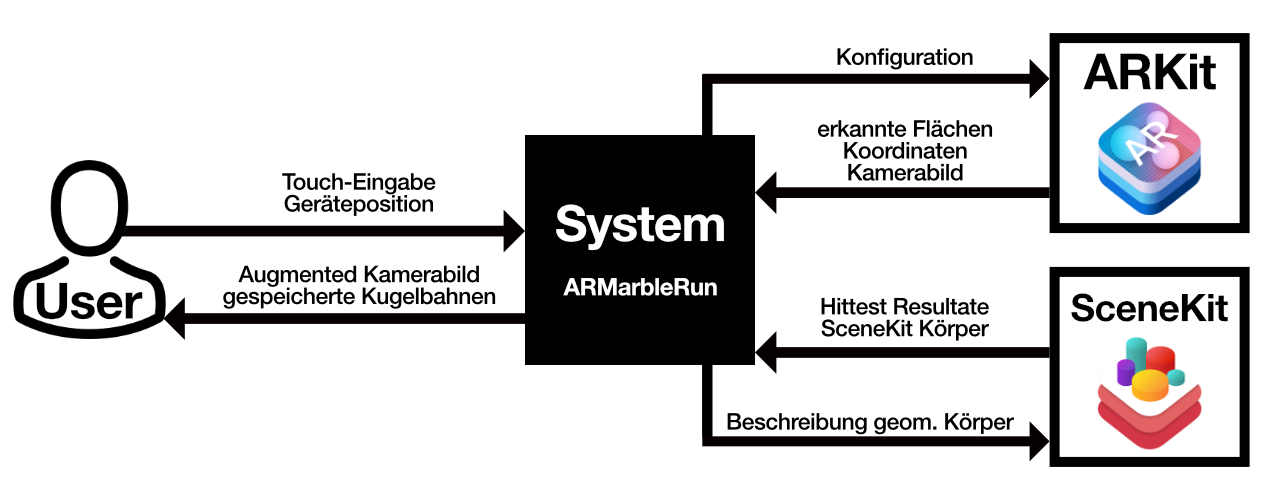
\includegraphics[width=\textwidth]{kontextdiagramm}
\end{figure}

\subsection{Systemvision}

Für Kugelbahnenthusiasten, cuboro Fans und solche die es noch werden wollen,
die ihre Kugelbahn mitnehmen wollen, planen wollen und nach Anleitung nachbauen wollen,
bietet unsere Kugelbahn App
mit Augmented Reality
eine komfortable, moderne und effiziente Methode seine Bahn zu planen oder zu bauen.
Anders als das offizielle cuboro Webkit,
ist die Kugelbahn mit der App mobil und man kann sie virtuell in einen realen Raum stellen.

\subsection{Architekturprinzipien}

Die zu entwickelnde Demo-App wird zu einem grossen Teil zum Selbstzweck erstellt.
Die App soll die ausgearbeiteten technologischen Möglichkeiten demonstrieren.
Der Code selber muss für an der entsprechenden Technik Interessierte hilfreich sein.
Dazu soll er informativ und verständlich sein.
Dies wird unter anderem mit \textbf{Selbstdokumentation} und der \textbf{Trennung von Verantwortlichkeiten} erreicht.
Die Trennung der Verantwortlichkeiten soll ausserdem dazu führen, dass einzelne Aufgaben/Teilprobleme gezielt studiert und wiederverwendet werden können.

\subsection{Taktiken}

Durch eine durchgehenden, starken Nutzung von Interfaces kann übersichtlich sichergestellt werden, welche Bestandteile der Software welche Aufgaben lösen. Die Interfaces sollen sprechene Methoden und Attributevariablen haben und wo notwendig mit Kommentaren ergänzt werden. Dieses Vorgehen hilft sowohl der Trennung von Verantwortlichkeiten und der Selbstdokumentation.

Weiter sollen Klassen möglichst klein und kohäsiv gehalten werden und zu zusammengehörigen Modulen gruppiert werden. Somit sollen interessante Stellen im Code rascher gefunden und verstanden werden. Das Vereinfacht die Wiederverwendung einzelner Module.

\subsection{Architekturstil}

Da die App monolithischen Charakter hat, also ohne Verbindungen nach Aussen und ohne Notwendigkeit zur Kommunikation mit verteilten Komponenten ist, fallen verteilte Stile (Client-Server, P2P usw.) weg.
Praktisch alle Abläufe in der App werden durch den Benutzer ausgelöst und führen zur Ausführung verschiedener Use Cases. Im Kern stehen die Kugelbahnen und deren Elemente.
Ein Stil nach dem Vorbild von Clean Architecture scheint daher passend zu sein: Events aus dem UI werden über Interfaces an verschiedene Interactor (Use Cases) weitergegeben, welche die Entities abrufen und bearbeiten.

Bei Recherchen stiessen wir auf die VIPER Architektur, welche versucht Clean Architecture spezifisch für iOS umzusetzen. Jeder Use Case ist ein VIPER Modul, das aus View, Interactor, Presenter, Entities und Wireframe (Router) besteht. Die Wireframes initialisieren ihr Modul und sind für das Aufrufen anderer Module verantwortlich. Der Interactor nutzt die globalen DataManager um Daten aufzurufen und für den Presenter bereitzustellen.

\begin{figure}
  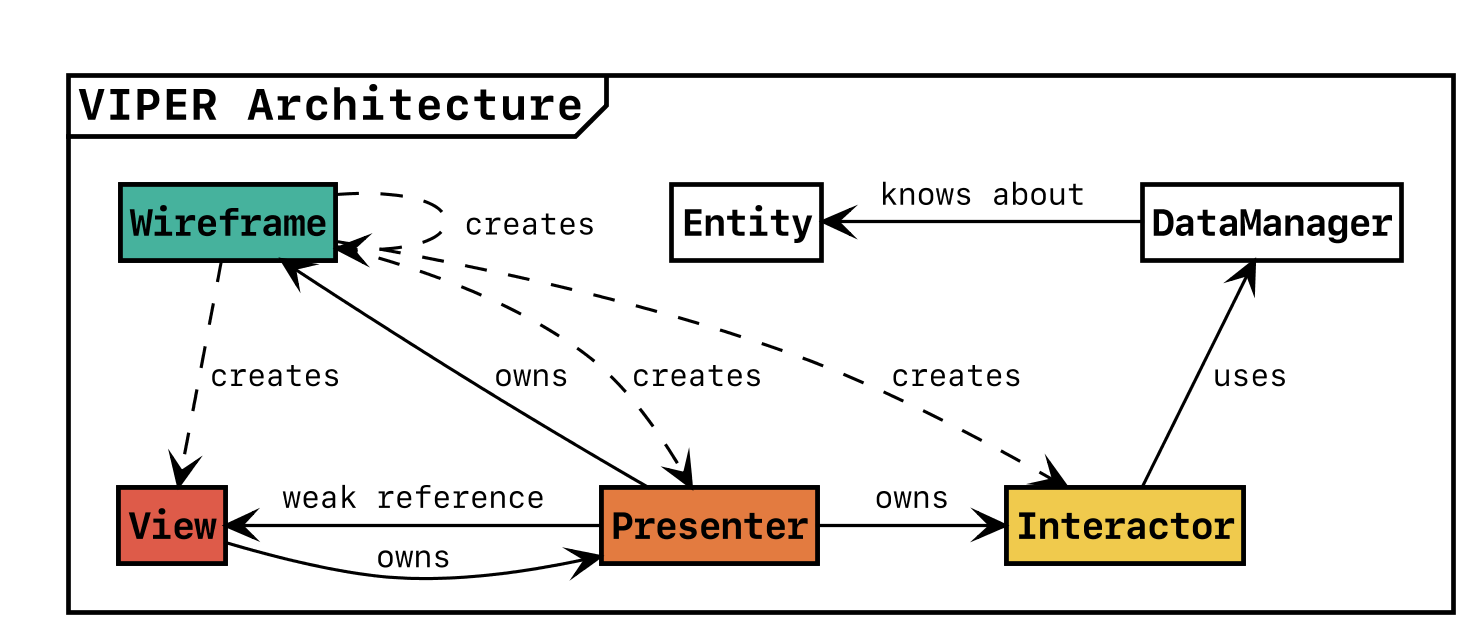
\includegraphics[width=0.8\textwidth]{viper-architecture}
\end{figure}

Die beiden wesentlichen Funktionen Bauanleitung (ARGuide) und Baumodus (AREditor) sind jeweils ein solches Modul. Sie teilen sich den DataManager, der Zugriff auf Kugelbahn- und Element-Entities hat. Daneben gibt es den Startbildschirm, bei dem der User den Modus wählen kann (SelectMode) und Listenansichten für Kugelbahnen (MarbleRunList) und Elemente (ElementList).

\begin{figure}
  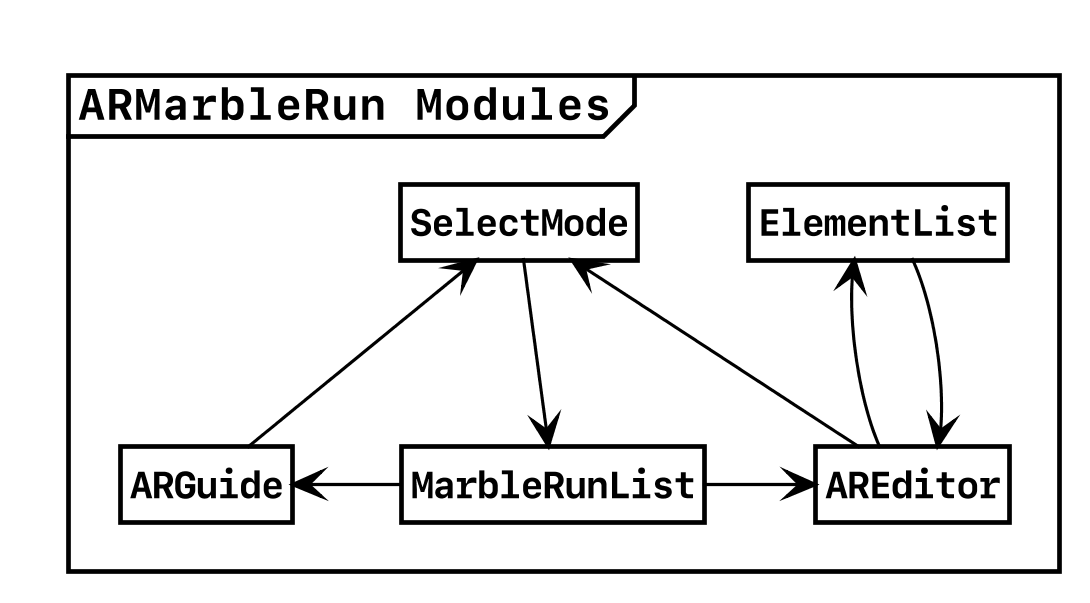
\includegraphics[width=0.5\textwidth]{viper-modules}
\end{figure}

\subsection{Systemsichten}

Alle Aktivitäten gehen von der View, bzw. vom Benutzer aus. Daher beginnt der folgende Fluss mit der View.

\begin{figure}
  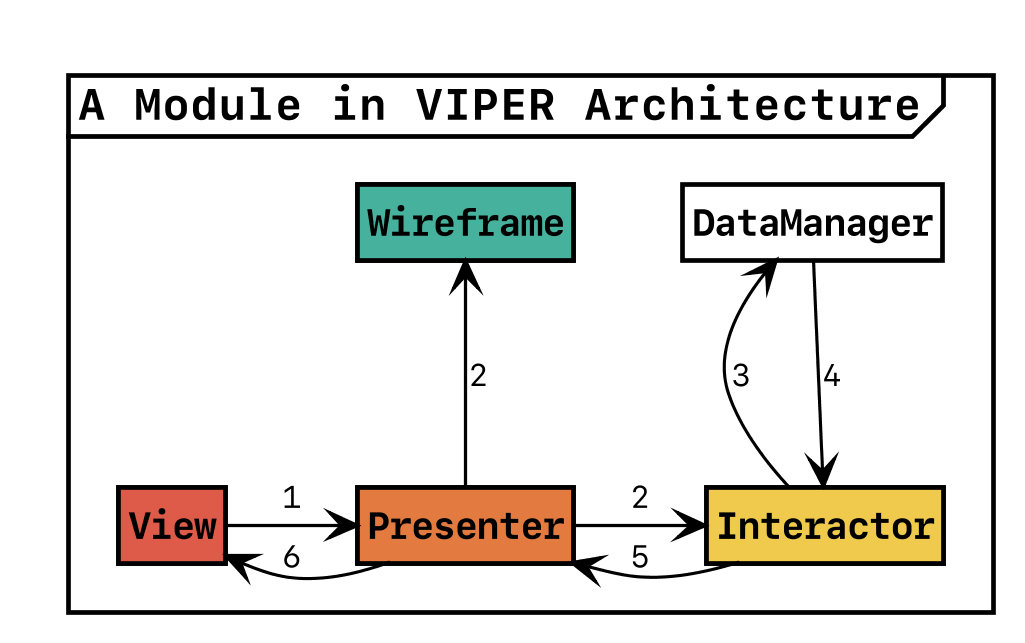
\includegraphics[width=0.5\textwidth]{viper-architecture-numbered}
\end{figure}

\begin{enumerate}
  \item Die View übergibt ein Event an den Presenter.
  \item Je nach Event wird entweder ein anderes Modul aufgerufen (via Wireframe) oder eine Anfrage nach Daten an den Interactor, der die Business Logik hat gerichtet.
  \item Der Interactor sendet einen Request nach Daten an den entsprechenden DataManager.
  \item Der DataManager gibt die gewünschten Entity Daten zurück.
  \item Der Interactor verarbeitet die Daten falls nötig und gibt sie an den Presenter weiter.
  \item Vom Presenter erhält die View nun Informationen, wie sie sich zu verändern hat.
\end{enumerate}

\subsection{Architekturentscheidungen}

Im folgenden zwei der wichtigsten Architekturentscheidungen:

\begin{table}
  \begin{tabular}{l p{13cm}}
    Issue         & 
      Der Benutzer soll zwischen den beiden Modi Baumodus und Bauanleitung wechseln können, ohne die virtuelle Kugelbahn neu im realen Raum zu platzieren. \\
    Alternatives  & 
      \begin{tabular}[t]{@{}p{13cm}@{}}
        Zwei Varianten:
        \begin{enumerate}
          \item Nur die relevanten UI Elemente (Buttons) ein-/ausblenden und eine Eventhandler Klasse verwenden, die ausgetauscht werden kann.
          \item Zwei getrenne Module machen, die sich die AR Szene mit den relevanten Informationen übergeben.
        \end{enumerate}
      \end{tabular} \vspace*{-\baselineskip}
      \\
    Outcome       & 2. Zwei getrennte Module. \\
    Rationale     &
      Eine saubere Trennung der unterschiedlichen Modi hilft der Nachvollziehbarkeit und Verständlichkeit des Codes und entkoppelt die Komponenten. Dies unterstützt ausserdem die Trennung der Verantwortlichkeiten und Erweiterbarkeit und bietet eine klarere Struktur. \\
  \end{tabular}
\end{table}

\begin{table}
  \begin{tabular}{l p{13cm}}
    Issue         &
      Die Elemente der aktuellen Kugelbahn müssen einerseits in der View als SceneKit Kindknoten der Kugelbahn zur Darstellung sein. Andererseits müssen sie in einem Konstrukt sein, das ihre logische Position und Nachbarn verwalten kann, um die Bauanleitung und Persistierung zu ermöglichen. \\
    Alternatives  &
      \begin{tabular}[t]{@{}p{13cm}@{}}
        Zwei Varianten:
        \begin{enumerate}
          \item Die SceneKit Knoten werden mit den notwendigen Informationen erweitert und zusammen mit logischen Koordinaten zusätzlich in einer Hashmap referenziert für die Business Logik.
          \item Die SceneKit Knoten werden rein auf ihre Funktion als UI Komponente reduziert und von zu persistierenden Entities getrennt.
        \end{enumerate}
      \end{tabular} \vspace*{-\baselineskip} \\
    Outcome       & 2. View und Entity trennen. \\
    Rationale     & 
      In Prototypen wurde Variante 1 versucht, dies führt jedoch zu starker Vermischung von Darstellung/View und der Business Logik. Die gewählte Variante stellt die Trennung von Verantwortlichkeiten sicher und erlaubt es zwischen der Darstellung von Persistierung von Kugelbahnen zu abstrahieren. Dadurch könnte das Datenformat geändert werden, ohne auch die Handhabung der 3D Element/Knoten komplett ändern zu müssen. \\
  \end{tabular}
\end{table}


}




}

\end{document}
